%; whizzy paragraph
%; whizzy-paragraph "^\\\\dancersection"
% -initex iniptex -latex platex -format platex -bibtex jbibtex -fmt fmt
% 以上 whizzytex を使用する場合の設定。

%     Tokyo Debian Meeting resources
%     Kansai Debian Meeting resources
%     Copyright (C) 2008 Junichi Uekawa
%     Copyright (C) 2008 Nobuhiro Iwamatsu

%     This program is free software; you can redistribute it and/or modify
%     it under the terms of the GNU General Public License as published by
%     the Free Software Foundation; either version 2 of the License, or
%     (at your option) any later version.

%     This program is distributed in the hope that it will be useful,
%     but WITHOUT ANY WARRANTY; without even the implied warranty of
%     MERCHANTABILITY or FITNESS FOR A PARTICULAR PURPOSE.  See the
%     GNU General Public License for more details.

%     You should have received a copy of the GNU General Public License
%     along with this program; if not, write to the Free Software
%     Foundation, Inc., 51 Franklin St, Fifth Floor, Boston, MA  02110-1301 USA

%   Pdf作成手順
% dvipdfmx debianmeetingresume2011-fuyu.dvi
%  preview (shell-command (concat "evince " (replace-regexp-in-string "tex$" "pdf"(buffer-file-name)) "&"))
% 画像ファイルを処理するためにはebbを利用してboundingboxを作成。
%(shell-command "cd image2011-fuyu; ebb *.png")


% progress memo:
% 2011/6-2011/11がマージ対象、関西は2011/6-2011/11(仮)
% イベント等でない場合は理由を書くこと。
% 必要な変更点は FIXME で記録しています。

%%ここからヘッダ開始。

\documentclass[mingoth,a4paper]{jsarticle}
\usepackage{monthlyreport}
\usepackage[dvips]{xy} % for advi workaround. Bug #452044

% 今回限りのコマンド for 201108 kansai
\definecolor{debianred}{rgb}{.780,.000,.211} % 199,0,54
\definecolor{debianblue}{rgb}{0,.208,.780} % 0,53,199
\definecolor{debianlightbackgroundblue}{rgb}{.941,.941,.957} % 240,240,244
\definecolor{debianbackgroundblue}{rgb}{.776,.784,.878} % 198,200,224
\definecolor{noir}{RGB}{3,3,36}
\definecolor{bleu}{RGB}{10,10,120}
\definecolor{bleuclair}{RGB}{17,17,150}
\definecolor{rouge}{RGB}{200,0,0}
\definecolor{jaune}{RGB}{255,255,0}
\definecolor{vert}{RGB}{0,255,0}
\definecolor{rougebg}{RGB}{160,0,0}
\definecolor{darkred}{rgb}{.7,0,0}
\newcommand{\textttc}[1]{\texttt{\color{rouge}#1}}
\newcommand{\textalert}[1]{{\color{darkred}{#1}}}
\usepackage{listings}
\lstset{basicstyle=\ttfamily}
\newcommand{\seprule}{\vspace*{-0.5em}\centerline{\rule{\linewidth}{0.3pt}}\vspace*{-0.5em}}
% 今回限りのコマンド for 201108 kansai

\begin{document}

\begin{titlepage}
\thispagestyle{empty}

\vspace*{-2cm}
あんどきゅめんてっど でびあん 2011年冬号\\
\hspace*{-2cm}

\includegraphics[width=210mm]{image2011-fuyu/debsen.pdf}\\
\hfill 2011年12月31日 初版発行

\rotatebox{10}{\fontsize{32}{32} {\gt 東京エリアDebian勉強会}}

\rotatebox{10}{\fontsize{32}{32} {\gt 関西Debian勉強会} }

\vspace*{-2cm}
\hfill{}
\includegraphics[height=6cm]{image200502/openlogo-nd.eps}
\end{titlepage}

\newpage
\thispagestyle{empty}\mbox{}
\newpage

% section の代わりの環境 -- 改訂する。
\renewcommand{\dancersection}[2]{%
\newpage
あんどきゅめんてっど でびあん 2011年冬号
%
% top line
\vspace{0.1mm}\\
{\color{dancerlightblue}\rule{\hsize}{2mm}}

%
% middle text
%
\begin{minipage}[t]{0.6\hsize}
\color{dancerdarkblue}
\vspace{1cm}
\section{#1}
\hfill{}#2\\
\end{minipage}
\begin{minipage}[t]{0.4\hsize}
\vspace{-2cm}
\hfill{}
\includegraphics[height=8cm]{image200502/openlogo-nd.eps}\\
\vspace{-5cm}
\end{minipage}
%
%
{\color{dancerdarkblue}\rule{0.74\hsize}{2mm}}
%
\vspace{2cm}
}


\begin{titlepage}
\includegraphics[height=252mm]{image2011-fuyu/2011-winter.eps}
%\thispagestyle{empty}
\end{titlepage}

\setcounter{page}{1}
\begin{minipage}[]{0.2\hsize}
 \definecolor{titleback}{gray}{0.9}
 \colorbox{dancerlightblue}{\rotatebox{90}{\fontsize{80}{80}
{\gt \color{dancerdarkblue}デビアン勉強会} }}
\end{minipage}
\begin{minipage}[]{0.8\hsize}
\hrule
\vspace{1mm}
\hrule
\setcounter{tocdepth}{1}
{\small
 \tableofcontents}
\vspace{1mm}
\hrule
\vspace{3cm}

\end{minipage}

% FIXME: 本文を追加すること。
% from debianmeetingresume200812.tex
\dancersection{Introduction}{上川 純一,山下 尊也}

\subsection{東京エリアDebian勉強会}

 Debian勉強会へようこそ。これからDebianの世界にあしを踏み入れると
 いう方も、すでにどっぷりとつかっているという方も、月に一回Debianについ
 て語りませんか?

 Debian勉強会の目的は下記です。

\begin{itemize}
 \item \underline{Debian Developer} (開発者)の育成。
 \item 日本語での「\underline{開発に関する情報}」を整理してまとめ、アップデートする。
 \item \underline{場}の提供。
 \begin{itemize}
  \item 普段ばらばらな場所にいる人々が face-to-face で出会える場を提供
	する。
  \item Debian のためになることを語る場を提供する。
  \item Debianについて語る場を提供する。
 \end{itemize}
\end{itemize}

 Debianの勉強会ということで究極的には参加者全員がDebian Packageをがりがり
 と作るスーパーハッカーになった姿を妄想しています。情報の共有・活用を通し
 て Debianの今後の能動的な展開への土台として、「場」としての空間を提供す
 るのが目的です。

\subsection{関西 Debian 勉強会}

 関西 Debian 勉強会はDebian GNU/Linux のさまざ
 まなトピック(新しいパッケージ、Debian 特有の機能の仕組、Debian 界隈で起
 こった出来事、などなど)について話し合う会です。

 目的として次の三つを考えています。
 \begin{itemize}
  \item MLや掲示板ではなく、直接顔を合わせる事での情報交換の促進
  \item 定期的に集まれる場所
  \item 資料の作成
 \end{itemize}

 それでは、楽しい一時をお楽しみ下さい。

% 201110 tokyo
\dancersection{Debian とはなにか?}{岩松信洋}
%-------------------------------------------------------------------------------
\index{debian}

この章は筑波大学さんでDebian勉強会を開催したときの資料です。

Debian勉強会を筑波大学さんで行うにあたり、たぶんLinuxやUbuntu、
Fedoraという言葉は知っているけど、
Debianは知らないって方がいるでしょう。
簡単にDebianとは何なのかを簡単に説明します。

\subsection{Debianとは?}

Debian Project の略称、またはDebian OSそのものを指す場合があります。
フリーかつオープンなOSを作る完全ボランティアベースのプロジェクトです。
歴史が長く保守的なLinuxディストリビューションの一つです。

公式開発者は約1000名。非公式な開発者やパッケージメンテナ、翻訳者などを入れると
5000名以上になります。世界のいたるところに開発者がいて、日本では約30名ほど公式
開発者が活動しています。また、日本の開発者が集まって活動している Debian JP Project
もあり、日本でのDebian環境のサポート、開発者育成、ユーザサポートなどを行なっています。

オープンソース・ライセンスの要件の定義(The Open Source Definition(OSD))は
DebianのDebianフリーソフトウェアガイドラインをベースとしたものです。

\subsection{特徴}

\subsubsection{フリーなソフトウェアで構成されている}
Debian プロジェクトはフリーソフトウェアを強く支持しています。
ソフトウェアには、いくつもの違ったライセンスが使われるので、
Debian フリーソフトウェアガイドライン (DFSG) を作って、
「何をもってフリーソフトウェアと言えるのか」の妥当な定義をしています。

\begin{itemize}
\item 何台のマシンにもソフトウェアをインストールしても良い。
\item 何人の人がソフトウェアを同時に使用しても良い。
\item 何個でもソフトウェアのコピーを作ってもいいし、それを誰にあげても構わない。(フリーもしくはオープンな再配布)
\item ソフトウェアの改変に対する制約が無い。(特定の通告を変えない事を除く)
\item そのソフトウェアを配布や売る事に対する制約が無い。
\end{itemize}

Debian の「main」ディストリビューションには、DFSG に適合したソフト
ウェアしか 入れる事を許されていません。
\footnote{http://www.debian.org/intro/free.ja.html より}

とはいっても、フリーではないアプリケーション
を使いたいユーザもいるので、そのようなユーザのためにcontrib、non-free
といったパッケージセクションを作って、できるだけ提供できるようにしています。

\subsubsection{オープンな開発をしている}
完全ボランティアの団体なので、特定の企業の力によってDebianの
方針が変更されたりすることがありません。
バグや議論経過なども全て公開されており、プロジェクトの方針等
はDebian公式開発者の選挙によって決まります。

\subsubsection{バイナリベースのディストリビューション}
ディストリビューションにはバイナリベースとソースベースの2種類があります。
前者は既にコンパイルされたパッケージを提供するディストリビューションで、
Debian や Redhat、Ubuntuなどがあります。
既にコンパイルされているので直ぐに使うことができますが、一定のルールに
よって最適化されているため、
使っているCPU向けに最適化されているとは限りません。しかし、同じアーキテク
チャならどの環境でも同じ問題が再現する
可能性があり、問題の共有が容易になります。
自分で使うソフトウェアは自分でコンパイルするというディストリビューションで、
代表的なものとしてGentooがあります。
パッケージにはソースコードはなく、コンパイルに必要な簡単なスクリプトがパッケー
ジに同梱されています。
このスクリプトで定義されている場所からソースコードをダウンロードし、コンパイルします。
これは自分に合わせたソフトウェアに最適化できるという利点があります。そのかわり
ソフトウェアを使うには時間がかかり、
問題があった場合でも他の環境では再現しにくいというデメリットもあります。

\subsubsection{豊富なパッケージ数}

Debianは多くのパッケージを提供しており、現在約3万パッケージのパッケージが利用可能です。
他のディストリビューションは、Gentooが15000パッケージ、Ubuntuだと10000パッケージ
\footnote{main と Universe がありますが、基本的にUbuntu側のサポートありなのはmainのみ。}
ほどあります。
Debian の変態的なところは、各アーキテクチャで同じバージョンのバイナリを
提供している事です。
リリース対象になっているアーキテクチャでパッケージが動作しない場合、ポーティング
を行い、開発元に取り込むように提案します。

%Gentoo? 約15000。あんなのビルドできるかわからないものも多くあるのでだめだろ。
%Ubuntu? main だけだと5000ぐらい?Universe とかありますが、基本的にUbuntu側のサポートはなし。

\subsubsection{ポリシーに基づいたパッケージ}
Debian で提供されているパッケージは Debian Pocilyという
パッケージングポリシーに基づいて作成されています。
このポリシーは厳格に決められており、違反しているパッケージ
はDebianにインストールされません。

\subsubsection{強力なパッケージングシステム}
Debianでは パッケージングシステムに dpkg というアプリケーションを使っており、deb という拡張子
がついたパッケージファイルをインストール、アンインストールします。
パッケージの依存関係管理がしっかりされており、depends(依存)、recommends(推奨)、
suggests(提案) などの項目によってコントロールしています。
パッケージマネージャのAPT (Advanced Package Tool) によって、インストールしたいパッケージに
依存しているパッケージがインストールされます。アンインストールも同様です。

\subsubsection{アップデートが容易}
Debian は約2年毎に安定版がリリースされます。Debian は
前回のバージョンからのアップデートをサポートしています。
例えば、2007年にリリースされた 4.0 から、最新版の 6.0 にアップデートするには、
4.0、5.0、6.0 と順にアップデートすることによって可能です。

\subsubsection{豊富なサポートCPUアーキテクチャ}
現時点で正式サポートCPUアーキテクチャは 11、次期リリースに向けてサポート
準備中が 10 あります。
サーバからPC、組み込みCPUまでサポートしています。
新しいCPUアーキテクチャをサポートするためのインフラもあるので、何がサポートしたいCPUが
ある人、debian-ports プロジェクト(http://www.debian-ports.org)に相談するとインフラを提供してくれるかもしれません。


\begin{minipage}[t]{0.5\hsize}

現在サポートしているアーキテクチャ。
\begin{itemize}
  \item amd64
  \item armel
  \item hurd-i386
  \item i386
  \item ia64
  \item kfreebsd-amd64
  \item kfreebsd-i386
  \item mips
  \item mipsel
  \item powerpc
  \item s390
  \item sparc
\end{itemize}

\end{minipage}
\begin{minipage}[t]{0.5\hsize}

サポート予定のアーキテクチャ
\begin{itemize}
  \item alpha
  \item armhf
  \item avr32
  \item hppa
  \item m68k
  \item powerpcspe
  \item s390x
  \item sh4
  \item sparc64
\end{itemize}

\end{minipage}

\subsubsection{Linux以外のカーネルもサポートする}

LinuxをカーネルとしたOS、Debian GNU/Linux だけではなく、
FreeBSDのカーネルを使ったOS Debian GNU/kFreeBSD
も提供しています。
Debian 開発者の中にはGNU Hurd, Minix, NetBSD カーネルを
ベースにした Debian を開発している人もいます。

\subsubsection{他のOSSプロジェクトと関連が強い}

Debian開発者と各OSS開発者が兼務していることが多く、他のOSS
プロジェクトと結び付きが強いです。パッケージメンテナ=開発元の開発者
ということが多いのが特徴です。自分の作ったソフトウェアをDebianに入れたい人が
多いようです。
また、大抵のDebian開発者は複数のプロジェクトに顔を出しているので、更にプロ
ジェクト間の結びつきが強いです。

\subsubsection{派生しているディストリビューションの多さ}
いままで説明した特徴によって、Debianから派生したディストリビューションが多く
あります。
有名なところでは、UbuntuやKnoppix、Vyatta (VPN/ネットワークファイアウォール)
などがあります。
現時点で129以上の派生ディストリビューション
\footnote{http://distrowatch.com/dwres.php?resource=independence 参照}
があり、Debianの live CD システムを使った小さい
ディストリビューションを入れるともっと多くなります。
また派生として分散させているだけでなく、派生したディストリビューションの
成果を本家であるDebianに取り組む仕組みもあります。
ちなみに2番目に多いのはFedoraベースの 63 です。

\subsection{まとめ}

\begin{itemize}
\item フリーである。
\item オープンな開発プロジェクトである。
\item 世界規模のボランティアベースのプロジェクトである。
\item バイナリベースのディストリビューションで、サポートしているパッケージ数が多い。
\item サポートしているアーキテクチャが多い。
\item Linux カーネルだけをサポートしていない。
\item 派生しているディストリビューションが多い。
\end{itemize}

\subsection{んで、どういう風に使えばいいの?}

個人的な見解ですと、

\begin{itemize}
\item 開発に使いたいなら、Debian か Gentoo。

アップストリームに近い位置にいるためです。
パッチなどがディストリビューション開発者経由で取り込まれやすい。

\item デスクトップやノートPCで使いたいなら Ubuntu。いろいろデスクトップとか弄りたいなら、DebianかGentoo。

2ch とかニコニコ動画みる程度なら Ubuntu で十分だと思います。もちろん Debian でも問題ありません。
プログラムを最適化したいとか、「Gnomeとかイラネ!他のデスクトップ環境が欲しい」という人なら、Debian かGentooをお薦めします。

\item サーバで使いたいなら、Debian。

無駄なものがインストールされてないから。

\end{itemize}
です。

ぜひDebianを使って、フィードバックをください。
そして開発に興味がある人は開発に参加してみてください。手取り足取り教えます。
みんなでDebianを良いものにしていきましょう。

% 201110 kansai
%------------------------------------------------------------------------------
\dancersection{翻訳で Debian に貢献しよう}{八津尾 雄介}
\index{ほんやく@翻訳}
\subsection{はじめに}
Debian を利用する以上, 英語との付き合いは避けて通れない問題だと思います. 英語の
文章を読むのが苦にならない人から, エラーメッセージさえ読む努力を放棄する人まで,
様々だとは思いますが, もっと英語ができればと思う事が誰でも少なからずあると思い
ます.

私は英語と付き合う第一歩として, 翻訳をおすすめします. 翻訳というと特殊技術だとか自
分には無理と身構えてしまう人も多いかもしれませんが, それほど敷居の高い作業ではあ
りません.

辞書と基本文法の知識さえあれば誰でもできる作業ですし, どうしても意味がとれない箇
所はメーリングリストなどへ投げれば誰かが答えてくるでしょう. ついでに Debian の知
識も身につくので, Debian Maintainer や Debian Developer を目指している人にとって
うってつけの自習教材ではないでしょうか?

オープンソースコミュニティ全体に言えることだと思いますが, 翻訳者の数は圧倒的に少
ないのが現状です.その主たる原因を私なりに分析してみました.
\begin{itemize}
	\item 読める人は訳さない
	\item 読めない人も訳さない
	\item 時間も手間もかかる地道な作業
	\item 貢献に対する見返りがあまりない(なかった)
	\footnote{パッケージ作業以外でのDebian への貢献を認める決議がなされました}
\end{itemize}

\index{DDP}
DDP\footnote{Abbr. Debian Documentation Project: http://www.debian.org/doc/ddp}に
はまだ翻訳されていない文章がたくさんあります. 翻訳をしながら Debian について学び,
 貢献し, そして英語力の向上に役立ててみませんか?

\subsection{翻訳メモリとは}
\index{ほんやくめもり@翻訳メモリ}
翻訳とは一般的に, 時間も手間もかかる地道な作業なわけですが, それをある程度軽減して
くれるのが翻訳メモリツールです.翻訳メモリとは, 原文と翻訳文のペアをデータベース化
したもので, 翻訳メモリツールは翻訳メモリから一致率の高い文章をサジェストする翻訳
支援ソフトです.翻訳メモリツールを指して翻訳メモリということもあります.

翻訳メモリはいわば実用文例集のようなもので, 機械翻訳とは根本的に違います.注意した
いのは, 翻訳メモリを作るのは訳者自身だということです. 翻訳メモリツールが参照する
のはあくまで, あなたが (もしくはメモリの提供元が) 過去に訳した文章であり, それに
ついての正確さは一切保証されていません.

\subsubsection{翻訳メモリを使うと何が嬉しいのか}
では, 翻訳メモリを利用することで得られるメリットとは何でしょうか.
\begin{itemize}
	\item 膨大な訳文を蓄積し使い回す事により作業効率が一気に高まる(作業の効率化)
	\item 複数人で翻訳作業を行う際の文体や訳語の微妙な違いを少なくする事ができる
	      (一定品質の保持)
	\item PO形式ではない場合でも原文の変更に追従しやすくなる(保守性の向上)
\end{itemize}

職業翻訳では翻訳メモリが広く利用されています. 翻訳家は業界標準の翻訳メモリである
 Trados などの利用率が高いようです. 一方, Debian で利用可能な翻訳支援ツールは
 poedit や gtranslator, OmegaT. webベースであれば Google Translator Toolkit など
があります. どれも翻訳メモリを使用するツールです.

\subsection{OmegaTとは}
\index{omegaT}
OmegaT とは先述の通りオープンソースで利用可能な翻訳メモリで, Java で開発されて
おりクロスプラットフォームです. 翻訳メモリには LISA\footnote{abbr. Localization
Industry Standarts Assosiation = ローカライゼーション産業の標準化団体}
が標準化している TMX\footnote{abbr. Translation Memory eXchange} というオープンな
XML を採用しており, Trados や SDLX をはじめとした他ツール間で翻訳メモリを相互運用
できます.

OmegaT では同梱版の Java を使うように推奨されていますが Debian でもパッケージを
提供しており, apt からインストールすることも可能です.

\paragraph{OmegaTの(一般的に言われる)良い点}
\begin{itemize}
	\item オープンソース
	\item コミュニティが活発
	\item 業界標準の TMX を使っている
	\item Windows的 (あるいはGnome的) な操作性
\end{itemize}

\paragraph{OmegaTの(私から見て)ダメな点}
\begin{itemize}
	\item 起動が遅い(=Java)
	\item Look and Feelが残念(=Java)
	\item ショートカットキーとニモニックが致命的にまずい
	\item hjklで移動できない ← 重要
\end{itemize}

という事で Java で開発されているという点と, vim じゃないという点以外は特に不満は
ありません. しかしながら, マウス操作を強制されるというのはあまり気持の良いもので
はありませんね.

\subsection{OmegaTの使い方}
ここでは, apt から Debian パッケージをインストールしたものとして話を進めていきた
いと思います. Debian Squeeze での現在のバージョンは 1.8.1 ですが皆さんは Wheezy
あるいは Sid を使っているはずですので(?) 2.3.0 前提で進めたいと思います.
基本的な使い方についてはお手軽スタートガイドを読めばわかりますのでここでは割愛し
ます.

\subsubsection{ファイルフォーマットについて}

OmegaT は次のフォーマットをサポートしています.
\begin{itemize}
	\item OpenDocument や OpenOffice.org
	\item プレーンテキスト
	\item .poファイル
	\item XHTML, HTML
	\item Microsoft Open XML
	\item 字幕ファイル(SRT)
	\item Android リソース
	\item LaTeX
	\item 他多数
\end{itemize}

\paragraph{サポート外のファイルを訳すには}
DebianDoc-SGML の利用は廃止にむかっているもののまだまだ sgml のドキュメントが存在
します. sgml は OmegaT によってサポートされていない形式です.\footnote{Java で利用
可能なオープンのパーサが無いという理由らしい}
OmegaT はサポートしない形式のファイルを翻訳対象のファイルに加えようとしても無視し
ます.では, OmegaT でサポートされないフォーマットのファイルを訳すにはどうすれば良
いでしょうか?

とりあえず訳したいという場合にはファイルの拡張子を OmegaT でサポートされているフ
ァイルの拡張子にしてしまえば訳すことができます. ただし, タグ付きの文書の場合は
タグの扱いに注意をしなければなりません. とりあえず *.txt にしておくというのが正
解のような気がします.

Debian 的な方法としては Gettext PO 形式に変換して翻訳するという方法がありますが,
 OmegaT 的にやろうと思うのであれば, ファイルフィルターを利用して近いフォーマット
として認識させる方法が良いでしょう.
例えば sgml を xhtml として読み込ませたい場合, "設定" から "ファイルフィルター"
を選択し, XHTML を選択した状態で "編集" をクリックします. それから "追加" をクリ
ックして "*.sgml" を "原文ファイルの構成名" へ追加します. こうする事で sgml ファ
イルが翻訳対象のファイルとして追加可能になります.

残念ながら独自のファイル定義を追加できるわけでは無いので, 今のところは拡張子を変
更して対応する場合と大きな違いはありません. ただ, 例にあるような sgml などのタグ
付きのファイルを編集する場合, タグの挿入などの便利な機能を使えるようなるので txt
 で扱うよりも少し楽になるはずです.

\subsubsection{分節化規則を変更する}
分節化された文章を見てみると, 中途半端な箇所で切られてしまっているような場合が
ままあります. 特にタグ付きの文章をプレーンテキストとして読み込ませると思わぬ所
で分節化されてしまいます. そのような自体に対処したり, ユーザーの好みに柔軟に対応
する為に, 分節化の規則をカスタマイズする事が可能です.

分節化の設定は "設定" の "分節化規則" から行えます. 分節化規則の定義は Java で
サポートされている正規表現を使用します.

この分節化規則は慎重に取り扱うべきでしょう. 途中で規則を変更してしまえばメモリの
一致率を下げる原因となるからです. 分節化規則は良く考えられて作られているので, 最
初はデフォルトのまま使用し, もし不満があれば何度が試験的な短めのドキュメントでテ
ストしながら徐々に自分の好みに合わせていけば良いでしょう. いきなり長文の翻訳に適
用してしまうと, 思わぬ不都合が起きた場合の対処が非常に面倒です.

\subsubsection{用語集を作成する}

用語集:グロッサリ は プロジェクトフォルダ内の glossary に置きます. (デフォルト
設定)翻訳中にでくわした用語をグロッサリへ登録しておけば訳語に統一感を持たせる事が
できます. 例えば "upstream" を訳す際に "開発元" とすべきか, "上流" とすべきか "ア
ップストリーム" とすべきかといったような事や "コンピュータ" と表記するか "コンピ
ューター" と長音を省略せず表記するかといったような曖昧になりやすい事は下読みの段
階でピックアップしグロッサリにしておくと良いでしょう.\footnote{一括で置換する手
法を使う人にとっては不要ですね…でも将来の為に作っておくと良いですよ}言うまでもな
く, 複数人で訳す場合はこれを共有すべきですね. Debian を デビアン と表記しないなど
"訳さない" 単語を登録しておくのも有効です.

グロッサリは OmegaT で直接編集はできません.\footnote{顧客からグロッサリを渡され
るような事があるので, 訳者が勝手に編集できないようにする配慮だと思われます}
作成/編集/メンテにはテキストエディタを使いましょう.

Debian JP では対訳表というのを作っていて(?)\footnote{私の知る限りでは放置中です}
OmegaT で利用できる形式にしてあるものも一応あります.\footnote{\url{http://w
ww.debian.or.jp/community/translate/}参照} とりあえずはこれを用語集として放り込ん
でおいても良いでしょう.

OmegaT のヘルプには何故か長々と OpenOffice を使ったグロッサリの作成方法が書かれて
います. グロッサリの元データが表計算ソフトで作られていたりワープロソフトで作ら
れていたりしないのであれば, テキストエディタで作った方が楽だと思います.

グロッサリのフォーマットは
\begin{commandline}
翻訳対象の言語[TAB]日本語[TAB]説明や注記
\end{commandline}
です. グロッサリのファイルは プロジェクトで使用しているものと同じエンコードで
保存し, ファイル名は "*.tab" とします. 私は面倒なので全て UTF-8 にし, グロッサ
リは "*.utf8" にしています.

実際にグロッサリを作成してみます. 例えばこんなファイルを作ってみましょう.

\begin{commandline}
Debian (tab) Debian
maintainer (tab) メンテナ
computer (tab) コンピュータ (tab) 長音省略
upstream (tab) 開発元 (tab) アップストリーム 上流 は避ける
Debian developer (tab) Debian 開発者
\end{commandline}

上記の例でわかるように, ソートされている必要は無いようです. これを OmegaT のプロ
ジェクトフォルダ内の glossary に配置します. 翻訳中の分節が含む完全一致した単語を
全て, 用語集ペインに表示します.
グロッサリは完全一致している必要があり, 活用形はピックアップできません.
例えば
\begin{quote}
Debian [tab] Debian
\end{quote}
があった場合, Debian's は ピックアップできません. ケースセンシティブではないので
debian は表示されます. このあたりの挙動を理解しながら良く使われる活用 - 例えば
上記の "Debian's" など - もある程度網羅すると良さそうです.

グロッサリに辞書ファイルを登録する事も可能ですが, 分節中の単語全てをリストアップ
し, まともな辞書であれば用語集ペインが溢れ返ってしまう上, 上記の通り活用まではカ
バーできない為あまりおすすめできません.

グロッサリは, 例えば "debian.utf8" ".utf8" など, 大雑把でもジャンル
分けしておいた方が再利用しやすくなります.


\subsubsection{辞書について}
実は私は OmegaT の辞書を使った事がありません. 普段は wine 上の PDIC で 英辞郎
を利用するか, 手元の電子辞書を使います. OmegaT では StarDict 形式の辞書ファイル
をサポートしていて, tab 区切りになっている辞書ファイルであれば stardicttools で
簡単に変換できます. せっかくなので英辞郎の辞書ファイルを StarDict の形式に変換
し使用してみましたが, 私の欲しい感じではありませんでした. 今後に期待です.

\subsection{翻訳メモリを活用する}
OmegaT では翻訳メモリを複数箇所に保持しています.

\paragraph{project/omegat フォルダ内}
\begin{itemize}
	\item{project\_save.tmx}
\end{itemize}
このフォルダ内には tmx ファイルのバックアップが作成されます. 翻訳作業を開始して
からの全ての分節が保存されています. プロジェクトとして実際に読み込まれているの
がこれです.

\paragraph{project/ 内}
\begin{itemize}
	\item{*\_omegat.tmx}
	\item{*\_level1.tmx}
	\item{*\_level2.tmx}
\end{itemize}
target ファイル生成時の source ファイルの内容に対応した翻訳メモリが作成されます.
それぞれのファイルフォーマットには微妙な差異があり, 用途によってわかれています.
level1 は文書情報のみが含まれています.
level2 は OmegaT 特有の情報が tmx タグ として保存されるので level2 の翻訳メモリ
に対応したアプリケーションでの利用が可能です.
omegat は OmegaT 特有のフォーマットなので他のアプリケーションからは利用できません.

\paragraph{project/tm フォルダ内}
過去のプロジェクトからメモリを流用したい時はこのフォルダに配置します. level1, level2
あるいは omegat のいづれかのファイルをいくつでも置いておく事が可能です.

翻訳メモリの内部を覗いでみましょう. フォーマットによって違いはありますが, だいたい
こんな風になっています.
\begin{verbatim}
	<tu>
		<tuv lang="lang1">
			<seg>lang1の分節</seg>
		</tuv>
	</tu>
	<tu>
		<tuv lang="lang2">
			<seg>lang2の分節</seg>
		<tuv>
	</tu>
\end{verbatim}

OmegaT のプロジェクトフォルダでは /source 内へのファイル配置は基本的に自由です. こ
のフォルダ内で "securing-howto" や "maint-guide" のように文書毎のフォルダを作り
管理するという方法がおすすめです. こうする事によって, いちいちマージやファイル
移動をしなくても用語集や翻訳メモリを共通で使えるようになります.

問題は翻訳メモリのサイズとソースファイルの量ですが, 試しに DDP からチェックアウトし
てきたファイルのうち, 不正なファイルだとエラーで弾かれるものを除き, 全てプロジェ
クトフォルダに放り込んでみました.
私が確認した限りでは問題なく動作していましたが, 読み込みに時間がかかるので同一
プロジェクトで扱うファイルは常識的な数に留めておく事が賢明です.

\subsubsection{機械翻訳を利用する}
機械翻訳はまだまだ使い物になりません. しかし, 短い文章の翻訳精度は向上しつつあり,
場合によっては て に を は を修正すればそのまま使えるような文章ができあがるような
場合もあります. うまく訳せない長目の文章でも, 特定の単語の意味がわからない場合な
どは有効な手段です. 別段必要な機能だとは思えませんが, あくまでも参考程度に利用す
るのであれば良いと思います.

\subsubsection{翻訳へ参加する}
翻訳を始めようと思ったら, まず Debian JP Documentation メーリングリストへ参加しま
しょう. 詳しくは \url{http://www.debian.or.jp/community/ml/openml.html} を参照する
か, 会場のスタッフへ尋ねてみてください. きっとあなたの世界が広がりますよ.


\subsection{まとめ}
現在勉強会当日の朝4時ですので, そろそろまとめに入らせて頂きます. OmegaT は数ある
翻訳メモリの中でもフリーで汎用性が高く, プロフェッショナルユースにも十分利用でき
るソフトウェアです.

翻訳作業全てを OmegaT で行う事を強制する事は望ましくありませんが, せめて翻訳メモ
リの使用を強く推奨し, コミュニティの資産としてメモリを蓄積できれば今後の翻訳作業
が加速する事は間違いありません.

また, 翻訳者の中にはマウスの操作を嫌う人が相当数いますので[要出典]是非ショートカ
ットキーのカスタマイズとニーモニックキーを採用して欲しいと思います.

% 201106 tokyo
%-------------------------------------------------------------------------------
\dancersection{Debian JP 定例会議処理系にXSLTを使ってみた}{上川純一}
%-------------------------------------------------------------------------------
\index{xsltproc}

\subsection{背景}

Debian勉強会の企画会議はIRCを中心として2006年に開始し、Debian JP の定例会
議として今も続いています。当初は決定事項などについてテキストファイルでま
とめるという形をとっていました。IRCでより効率よく議論する方法を模索した結
果、議論しながら議事録を編集するというスタイルが確立し、それを支援するた
めのツールを整備しました。

議事録のソースは議長がXMLで記述して、議論の最中は非同期にJavascriptで内
容が更新されるHTMLファイルを利用します(世間一般ではAJAX的とでもよぶよう
です)。

IRCでの定例会議の議論の前と後には議事案と議事録をメーリングリストにおくっ
ています。メーリングリストにメールでなげる際には、テキストフォーマットに
して送っています。

あと、現在用途がないですが、\LaTeX 経由でPDF形式での出力などもサポートし
ています。

現在の実装は歴史的な経緯によりXMLの処理系は dancer-xml ライブラリと
boostを利用したC++のプログラムになっています。
dancer-xml\cite{dancer-xml} は10年前に若気のいたりで実装したXML風文書のパー
サーです。一部エンティティーまわりなど真面目に実装していない部分があるた
め、適切な処理がなされていないことがありますが、僕の好みに空白文字処理は
チューニングされており快適です。

今回の挑戦は、独自C++コードベースをXSLTにのせ替えてみるという挑戦です。

\begin{figure}[ht]
 \begin{center}
  \includegraphics[width=0.5\hsize]{image201106/ircsystem.eps}
 \end{center}
\label{fig:ircsystem-general}\caption{IRC 会議システムのデータ形式の概要}
\end{figure}

\subsection{XSLTってどんな言語?}

XSLTはXMLで記述するXML処理言語です。

XSLT規格には1999年に策定されたXSLT 1.0 と、2007年ごろのXSLT 2.0があります。
今回は実装が十分枯れていると思われる XSLT 1.0 の処理系を採用しました。
XSLT2.0のDebianで利用できる実装としては libsaxonb-javaがある
ようですが、今回は調査していません。

プログラムを書くときにすべき文書としては、XSLT自体の1999年に策定された規
格\cite{xslt1999}と、XSLTの中で記述できるXPATHの規格\cite{xpath1999}を参
照するとよいでしょう。

XSLTだけではあまり高度なプログラミングはできないんじゃないかと思われるか
もしれませんが、関数型言語として十分な機能を提供できる力はあるようです
\cite{fxslt2003}。

\subsection{Debian で利用可能な XSLT処理系}

Debianで幅広く使われていて安定しているとおもわれるのと、簡単に利用できる
という理由で処理系として xsltproc を採用しました。

Debian での xsltproc のインストールは簡単
\begin{commandline}
$ apt-get install xsltproc
\end{commandline}
%$

コマンドラインで以下のように実行すると標準出力に処理済みXMLが出力されます。

\begin{commandline}
$ xsltproc [スタイルシート] [処理するXMLファイル]
\end{commandline}
%$

\subsection{具体例:HTML}

それでは、HTML出力の場合を見てみましょう。
\url{meetinglog:html.xsl}です。
XML文書からHTML文書を生成するにはそれなりに便利な言語です。

前半のコードをそのまま掲載します。
これは、XMLドキュメント全体にマッチするルールを記述しはじめるまでの部分
です。
XML名前空間として、デフォルトをHTML、xslをxsltの名前空間に割り当てていま
す。

xml:output で出力形式をHTMLと指定することでXMLヘッダが出力されずに便利で
す。

\begin{commandline}
<?xml version="1.0"?>
<!DOCTYPE xsl:stylesheet>
<xsl:stylesheet version="1.0"
  xmlns:xsl="http://www.w3.org/1999/XSL/Transform"
  xmlns="http://www.w3.org/1999/xhtml">
  <xsl:output method="html" />
  <xsl:template match="/">
    <html>
      <head>
\end{commandline}

他にXSLTの特徴的なところは、value-of で値をとってきています。XPATH
の書式で指定していますが、
\begin{commandline}
	<h1><xsl:value-of select="meetinglog/head/title"/></h1>
\end{commandline}

は、XML文書の以下のようなエレメントに入っている値を抽出します。
\begin{commandline}
 <meetinglog>
   <head>
     <title>タイトル</title>
   </head>
 </meetinglog>
\end{commandline}

議事録の場合のメインループは、各議事に対しての処理です。
xslのxsl:for-eachをつかい、XMLのエレメントノードの数だけループします。
HTMLタグはそのまま出力されますが、もしHTMLのアトリビュートなどをXSLTで生
成したい場合は、xsl:element を使ってエレメントを生成します。

position()関数は現在のエレメント番号をくれるのでこういう場合に便利です。

\begin{commandline}
           <xsl:for-each select="meetinglog/body">
	      <tr>
		<th>
		  <xsl:element name="a">
		    <xsl:attribute name="href">#gian<xsl:value-of select="position()" /></xsl:attribute>
		  </xsl:element>
		  議案<xsl:value-of select="position()" />
		</th>
		<td class="bodytitle">
		  <xsl:value-of select="./title" />
		</td>
 ....
 </xsl:for-each>
\end{commandline}

\subsection{具体例:Text出力}

Text出力の場合もみてみましょう。
\url{meetinglog:txt.xsl}
テキスト出力をしようとしはじめると若干苦しくなってきます。できないわけで
はないのですが、空白文字の処理のルールを僕がいまいち理解できていないのと、
コードがそのままテンプレートとして出力されるのでインデンテーションが適切
にできないのがつらいところです。

xsl:output で出力がテキスト形式であると指定するとXMLヘッダが出力されず便
利です。

ヘッダ部分で、毎回 xsl:text で改行などを入力するのが面倒なので、ENTITY を
定義して省略できるようにしています。この記法が正しいのかどうかは不明です。

\begin{commandline}
<?xml version="1.0"?>
<!DOCTYPE xsl:stylesheet [
<!ENTITY space  "<xsl:text xmlns:xsl='http://www.w3.org/1999/XSL/Transform'> </xsl:text>">
<!ENTITY indent "<xsl:text xmlns:xsl='http://www.w3.org/1999/XSL/Transform'>  </xsl:text>">
<!ENTITY cr     "<xsl:text xmlns:xsl='http://www.w3.org/1999/XSL/Transform'>
</xsl:text>">]>
  <xsl:stylesheet version="1.0"
    xmlns:xsl="http://www.w3.org/1999/XSL/Transform"
    xmlns="http://www.w3.org/1999/xhtml">
  <xsl:output method="text" />
  <xsl:template match="/">
    <xsl:text>-----------------------------------------------------------------------
概要
-----------------------------------------------------------------------
\end{commandline}

本文のコアとなる本文の内容ですが、読めたものではないです。
悩んだところとしては、文章が空白かどうかチェックするのに
string-length(normalize-space())をつかっていて、それがいまいちただしいの
かどうか自信がないところ。

\begin{commandline}
    <xsl:for-each select="meetinglog/body">
-----------------------------------------------------------------------
[<xsl:value-of select="position()" />.&space;<xsl:value-of select="./title" />]
-----------------------------------------------------------------------

目的: &cr;<xsl:value-of select="./aim" />&cr;
&cr;<xsl:if
 test="string-length(normalize-space(./previous))>1"
 >前回までの経緯:&cr;<xsl:value-of select="./previous"
 disable-output-escaping="yes" />&cr;&cr;</xsl:if>
<xsl:if test="string-length(normalize-space(./discussed))>1"
 >議論:&cr;<xsl:value-of select="./discussed"
 disable-output-escaping="yes" />&cr;&cr;&cr;
</xsl:if>
</xsl:for-each>
\end{commandline}

残念ながらC++で実装していた文字をメールの70文字幅くらいにきれいにまとめ
るというロジックが欠落しています。めんどくさすぎる。

\subsection{具体例:\LaTeX}

\LaTeX 出力をみてみましょう。
\url{meetinglog:latex.xsl}

ヘッダ部分はどうぜ\LaTeX{}のヘッダなのと何度もでてきているのでメインループ
だけ。
\begin{commandline}
    <xsl:for-each select="meetinglog/body">

      \discussion{<xsl:value-of select="./title" />}{<xsl:value-of
 select="./aim" />}{<xsl:value-of
 select="translate(./previous,'#&amp;','--')"
 disable-output-escaping="yes" />}{<xsl:value-of
 select="translate(./discussed,'#&amp;','--')"
 disable-output-escaping="yes" />}
    </xsl:for-each>
\end{commandline}

個人的な感想ですが、自分で書いておきながら後で読み返す気力が沸きません。

現在実装できていない点として、\LaTeX{}で使えない文字列\verb!#<>&!などの文
字列のエスケープがあります。今はハイフンに変更してお茶を濁しています。

XPATHには文字列置換のためのtransform()関数がありますが、一文字を一文字に置換
することしかできません。今回行いたいのは一文字を複数文字に置換することな
のでそれでは機能が不十分です。

\subsection{仮の定量的な比較}

現状すべての機能をおきかえているわけではないので、妥当な比較ではないです
が、C++の処理とXSLTのコードの比較をしてみると
(\ref{tab:xsltcxximplementationdiff})、
XSLTのほうが行数は少ないことがわかります。

\begin{table}[ht]
 \caption{lines of code for each implementation}
 \label{tab:xsltcxximplementationdiff}
\begin{center}
  \begin{tabular}{|c|c|c|}
 \hline
 & c++ & xslt \\
 \hline
 txt & 151 & 53\\
 html & 157 & 99 \\
 latex(PDF) & 158 & 87 \\
 \hline
 \end{tabular}
\end{center}
\end{table}

\subsection{結論}

XSLTを使うことでメンテナンスする行数は少なくなります。しかし、XPATH /
XSLT により提供されている機能が制限されているため、その中で実現しにくい
機能についてはがんばるか提供を諦めるのか、難しい判断を迫られます。

\begin{thebibliography}{0}
 \bibitem{fxslt2003} Dimitre Novatchev, ``Functional programming in XSLT
	 using the FXSL library,'' Extreme Markup Languages 2003.
 \bibitem{xslt1999} James Clark, ``XSL Transformations (XSLT)
	 Version 1.0,'' W3C Recommendation 16 November 1999.
	 \url{http://www.w3.org/TR/xslt}
 \bibitem{xpath1999} James Clark, Steve DeRose, ``XML Path Language
	 (XPath) Version 1.0,'' W3C Recommendation 16 November 1999.
	 \url{http://www.w3.org/TR/xpath/}
 \bibitem{dancer-xml} Junichi Uekawa, ``dancer-xml - Simple
	 non-comformant XML parsing library,'' 2000.
	 \url{http://www.netfort.gr.jp/~dancer/software/dancer-xml.html}
\end{thebibliography}

% 201106 tokyo
%-------------------------------------------------------------------------------
\dancersection{DebianでSphinxとDoxygenを使ってみた}{まえだこうへい}
%-------------------------------------------------------------------------------
\index{sphinx}
\index{doxygen}

\subsection{最近の流行りのようです}

Python関連のプロジェクトやエンジニアを中心に最近流行っているようです。
Sphinx-Users.jpのサイトを見る\footnote{\url{http://sphinx-users.jp/example.html}}と、
2011年6月現在、Sphinxのデフォルトテーマだけでなく、カスタムテーマやオリジナルテー
マを使った、50弱の日本語のサイトが紹介されています。

\subsubsection{reSTとSphinxの概要}

SphinxはreST(reStructuredText)という軽量マークアップ言語で書いたソースを
様々なフォーマットのドキュメントに変換・生成するためのツールです。
出力可能なフォーマットには、HTML、 \LaTeX 、PDF、ePub、man、平文テキスト、JSONなどがあります。

\subsubsection{reSTのサンプル}

試しに、東京エリアDebian勉強会のページをreSTで書くとこんな感じになります。

\begin{commandline}
========================
 東京エリアDebian勉強会
========================


背景
====

2005年当初、東京近辺で、類似の勉強会は存在していませんでした。
Debian について語る場所を提供するため、 Debian 勉強会を開催します。
この勉強会では毎回事前課題を設定しています。
その課題を提出することが参加の条件です。
参加する方は宴会の都合もありますので、事前に登録してください。
また、当日はDebianについての知識に関した簡単な試験を実施するので、
勉強会の会場には筆記用具を持参ください。

現在、 Debian 勉強会は
`Debian JP Project <http://www.debian.or.jp/>`_
のメンバーが Debian JP の公式なイベントとして運営しています。

次回の勉強会
============

* `2011年6月勉強会(第77回東京エリアDebian勉強会) <2011-06.html>`_
* `第48回関西Debian勉強会 <http://wiki.debian.org/KansaiDebianMeeting20110626>`_
* `毎週開催のハックカフェ <hackcafe.html>`_
(snip)
\end{commandline}

具体的な書式については、Sphinx-Users.jpのドキュメント\footnote{\url{http://sphinx-users.jp/doc.html}}を参照してください。

\subsection{Sphinxを使うきっかけ}

graphvizのdot言語と似た書式でブロック図を生成できるblockdiagシリーズ
\footnote{\url{http://blockdiag.com/}}というpythonで書かれたツールがあります。
最近、岩松さんにスポンサーをお願いして、これらのDebianパッケージ化を行っ
ています。これらのSphinx拡張機能(spyhinxcontrib-blockdiagなど)を使うと、
Sphinxで生成するドキュメントの中にブロック図を埋め込むことができます。
このblockdiagシリーズが便利なので、Sphinxを使いだしたようなものです。

また、仕事では基本的にMS Office、とくにExcelやPowerPointでの文書作成がほ
とんどなのですが、今期の最初に「もうMS Officeなんてでやってられっかー、
Sphinxで作ろうぜ!」と、プロジェクト内で提案して使い始めました。私個人で
作る分には \LaTeX でも良いのですが、他の二人はWindowsしか普段触ったことがな
い上、文書と言えば上述のとおり、ExcelかPowerPoint、という状態です。まっ
たく使ったことがない人に \LaTeX 文書を作成させるのは敷居が高すぎます。しか
し、reST \& Sphinxなら割と簡単に入門できる上、Windowsとの共同作業の環境
を整えるのもメンドイけど( \LaTeX 環境を整えるよりも)楽だった、という経緯です。\footnote{Windowsは改めてマンドイと思いました。\url{http://d.hatena.ne.jp/mkouhei/20110521/1305905297}}

\subsection{Debianで使ってみる}

試しに先ほどの東京エリアDebian勉強会のホームページをreSTで書いたものをSphinxで管理してみましょう。

まずはpython-sphinxパッケージをインストールしておきます。
\begin{commandline}
$ sudo apt-get install python-sphinx
\end{commandline}

emacsを使う場合は、python-docutilsパッケージをインストールしておけば、拡張子がrstかrestの場合、rst.elによって自動的にReSTモードになります。

\begin{commandline}
$ sudo apt-get install python-docutils
\end{commandline}

Sphinxプロジェクトを作ります。プロジェクト用のディレクトリを作ります。

\begin{commandline}
$ mkdir tokyodebian
$ cd tokyodebian
\end{commandline}

作成したディレクトリに移動して、\texttt{sphinx-quickstart}コマンドを実行
します。
\begin{commandline}
$ sphinx-quickstart
\end{commandline}

このコマンドを実行すると対話形式で聞かれます。htmlを生成するので、
Project Name, Author name(s), Project Version以外はデフォルトのまま
(Enterを押下)で良いでしょう。(表\ref{tab:sphinx-quickstart})

\begin{table}[h]
{\scriptsize
 \caption{sphinx-quickstartの設定項目}\label{tab:sphinx-quickstart}
  \begin{tabular}{|l|c|c|}
    \hline
    設定項目 & デフォルト値 & 設定例 \\
    \hline
    Root path for the documentation & . & デフォルト \\
    Separate source and build directories (y/N) & n & デフォルト \\
    Name prefix for templates and static dir & \_ & デフォルト \\
    Project name: & & Tokyo Debian Meeting \\
    Author name(s) & & Debian JP Project \\
    Project version & & 1.0 \\
    Project release & 1.0 & デフォルト \\
    Source file suffix & .rst & デフォルト \\
    Name of your master document (without suffix) & index & デフォルト \\
    Do you want to use the epub builder (y/N) & n & デフォルト \\
    autodoc: automatically insert docstrings from modules (y/N) & n & デフォルト\\
    doctest: automatically test code snippets in doctest blocks (y/N) & n & デフォルト \\
    intersphinx: link between Sphinx documentation of different projects (y/N) & n & デフォルト \\
    todo: write ``todo'' entries that can be shown or hidden on build (y/N) & n & デフォルト \\
    coverage: checks for documentation coverage (y/N) & n & デフォルト\\
    pngmath: include math, rendered as PNG images (y/N) & n & デフォルト \\
    jsmath: include math, rendered in the browser by JSMath (y/N) & n & デフォルト \\
    ifconfig: conditional inclusion of content based on config values (y/N) & n & デフォルト\\
    viewcode: include links to the source code of documented Python objects (y/N) & n & デフォルト \\
    Create Makefile? (Y/n) & y & デフォルト \\
    Create Windows command file? (Y/n) & y & デフォルト \\
    \hline
  \end{tabular}
}
\end{table}

先ほどのtokyodebian.rst(および、hackcafe.rst, 2011-06.rst)をコピーします。
\begin{commandline}
$ cp -i ~/*.rst .
\end{commandline}

自動的に生成されるindex.rstにこれらを追記します。\footnote{拡張子不要です。}
\begin{commandline}
$ sensible-editor index.rst
---
.. Tokyo Debian Meeting documentation master file, created by
   sphinx-quickstart on Fri Jun 17 13:39:53 2011.
   You can adapt this file completely to your liking, but it should at least
   contain the root `toctree` directive.

Welcome to Tokyo Debian Meeting's documentation!
================================================

Contents:

.. toctree::
   :maxdepth: 2

   tokyodebian  ←追加
   hackcafe  ←追加
   2011-06  ←追加

Indices and tables
==================

* :ref:`genindex`
* :ref:`modindex`
* :ref:`search`

\end{commandline}

コンパイルします。
\begin{commandline}
$ make html
sphinx-build -b html -d _build/doctrees   . _build/html
Running Sphinx v1.0.7
loading pickled environment... done
building [html]: targets for 4 source files that are out of date
updating environment: 0 added, 4 changed, 0 removed
reading sources... [ 25%] 2011-06
reading sources... [ 50%] hackcafe
reading sources... [ 75%] index
reading sources... [100%] tokyodebian

looking for now-outdated files... none found
pickling environment... done
checking consistency... done
preparing documents... done
writing output... [ 25%] 2011-06
writing output... [ 50%] hackcafe
writing output... [ 75%] index
writing output... [100%] tokyodebian

writing additional files... genindex search
copying static files... done
dumping search index... done
dumping object inventory... done
build succeeded.

Build finished. The HTML pages are in _build/html.
\end{commandline}

\_build/html/ディレクトリの下にreSTから生成されたHTMLファイルができます。

\subsection{Debianの日本語環境での状況}

HTMLの場合は日本語も問題なく表示できました。他のフォーマットはどうでしょうか。
結果は下記のとおりです。(表\ref{tab:format})

\begin{table}[h]
 \caption{フォーマット毎のビルド結果}\label{tab:format}
 \begin{center}
{\scriptsize
  \begin{tabular}{|l|c|}
    \hline
    フォーマット & 結果 \\
    \hline
    html & OK \\
    epub & OK (ただし、CSSは反映されない)\\
    text & OK \\
    man & OK \\
    latex & OK \\
    latexpdf & NG \\
    \hline
  \end{tabular}
}
 \end{center}
\end{table}

上記のとおり、 \LaTeX からPDFへの生成がうまくできません。

\begin{commandline}
(snip)
! PACKAGE INPUTENC ERROR: UNICODE CHAR \U8: NOT SET UP FOR USE WITH LATEX.

SEE THE INPUTENC PACKAGE DOCUMENTATION FOR EXPLANATION.
Type  H <return>  for immediate help.
 ...

l.119 \chapter{東京エリアDebian勉強会}

?
(snip)
\end{commandline}

これは生成される\LaTeX 文書がUTF-8であるためです。Debian JP Projectでの課題にもなっていますが、現状のDebianの \TeX 系では日本語のUTF-8は未対応です。

また、日本語を使っていなくても、GIFイメージを''\texttt{.. image::}''で読み込んでいる場合にPDFの生成に失敗するようです。

\subsubsection{rst2pdfを使う方法}
reSTからPDFへの生成には、 \LaTeX 経由での方法以外に、rst2pdfというツールを使う方法もあります。まず、rst2pdfパッケージをインストールします。

\begin{commandline}
$ sudo apt-get install rst2pdf
\end{commandline}

インストール後、先ほど作ったSphinxのプロジェクトディレクトリの直下にconf.pyという設定ファイルがあるので、この中のextensionsに下記を追記します。
\begin{commandline}
extensions = ['sphinx.ext.autodoc','rst2pdf.pdfbuilder']
\end{commandline}

PDFのオプションを追記します。
\begin{commandline}
pdf_documents = [
        ('index',u'TokyoDebianMeeting', u'Tokyo Debian Meeting', u'Debian JP Project'),
]
pdf_stylesheets = ['sphinx','kerning','a4','ja']
pdf_font_path = ['/usr/share/fonts/']
pdf_language = 'ja_JP'
\end{commandline}

Makefileに下記を追記します。
\begin{commandline}
pdf:
        $(SPHINXBUILD) -b pdf $(ALLSPHINXOPTS) $(BUILDDIR)/pdf
        @echo
        @echo "Build finished. The pdf files are in $(BUILDDIR)/pdf."
\end{commandline}

ja.jsonファイルを作ります。
\begin{commandline}
{
  "fontsAlias" : {
    "stdFont": "ttf-japanese-gothic",
    "stdBold": "ttf-japanese-gothic",
    "stdItalic": "ttf-japanese-mincho",
    "stdBoldItalic": "ttf-japanese-mincho",
    "stdMono": "ttf-japanese-gothic"
  }
}
\end{commandline}

make pdfを実行すると、\_build/pdf/TokyoDebianMeeting.pdfが生成されます。日本語の表示も問題ありません。詳細については、/usr/share/doc/rst2pdf/manual.pdf.gz にマニュアルがあるので、これの「Section 18 Sphinx」のページを参照してください。なお、この場合はmake latexpdfではうまくいかなかったGifファイルの読み込みは問題ありません。

しかし、この方法ではsphinxcontrib.*diagを使うと、ビルドに失敗するという別の問題があります。

\subsection{Doxygenとは}

さて、今回のもう一つのドキュメント生成ツールであるDoxygenについて見てみます。
Doxygenはソースコードを解析してドキュメントを生成するツールです。対応する言語は
C/C++、Java、Python、C\#、Objective-Cなど
をサポートし、DやPHPも部分的にサポートしています。

一方、生成可能なフォーマットは、
HTML、 \LaTeX 、RTF(MS-Word)、PostScript、PDF、manなどがあります。

\subsubsection{Debianで使ってみる}
今回は、Debian勉強会参加登録システムのソースコードからドキュメントを生成してみることにします。

Debianパッケージがあるので、doxygenパッケージをインストールします。

\begin{commandline}
$ sudo apt-get install doxygen
\end{commandline}

次に、ソースツリーのルートディレクトリに移動し、設定ファイルを生成します。

\begin{commandline}
$ cd monthly-report/utils/gae/
$ doxygen -g .doxgen.conf
\end{commandline}

Debian勉強会参加登録システムはPythonなので、最低限次の設定項目の設定を行
います。(表\ref{tab:doxygen})

\begin{table}[ht]
\begin{center}
{\scriptsize
 \caption{Doxygenの設定項目}\label{tab:doxygen}
  \begin{tabular}{|l|c|c|}
    \hline
    設定項目 & デフォルト値 & 設定例 \\
    \hline
    PROJECT\_NAME & & Tokyo Debian Meeting \\
    PROJECT\_NUMBER & & 1.0 \\
    OUTPUT\_LANGUAGE & English & Japanese \\
    TAB\_SIZE & 8 & 4 \\
    INPUT & & . \\
    FILTER\_PATTERNS & & *.py \\
    \hline
  \end{tabular}
}
\end{center}
\end{table}

\texttt{doxygen}コマンドを実行します。
\begin{commandline}
$ doxygen .doxygen.conf
\end{commandline}

すると、monthly-report/utils/gae/ディレクトリ以下に、html, latexディレク
トリができます。htmlディレクトリ以下にはHTML形式で、latexディレクトリ以
下には、 \LaTeX 及びPDF形式でドキュメントが生成されます。

w3mでhtml/index.htmlを見ると、以下のような画面が表示されます。

\begin{center}

\includegraphics[width=9.5cm]{image201106/doxygen0.eps}
\end{center}

``クラス''リンクをクリックするとクラスの一覧が展開されます。
\begin{center}

\includegraphics[width=9.5cm]{image201106/doxygen1.eps}
\end{center}

例えば、''admin\_event::EditEvent''のリンクをクリックすると、admin\_event::EditEventクラスについてのドキュメントを見ることができます。
\begin{center}

\includegraphics[width=9.5cm]{image201106/doxygen2.eps}
\end{center}

Doxygenについての詳細はdoxygen.jp\footnote{\url{http://www.doxygen.jp/manual.html}}のマニュアルを参照してください。

\subsubsection{Sphinxとの連携}

breathe\footnote{\url{https://github.com/michaeljones/breathe}}というツールを使
うと、reST/SphinxからDoxygenに連携できるようです\footnote{\url{http://sphinx.shibu.jp/faq.html}}。なお、Debianパッケージにはなってません。

\subsection{まとめ}
ソースコードからドキュメントを作るDoxygen, またドキュメントの作成自体を簡単にするSphinxを使うと、大変でなかなかやりたがらないドキュメントの作成の敷居を低くすることができます。また冒頭で紹介したSphinx拡張としても使える*diagシリーズや、まだDoxygenとSphinxを連携するBreatheを使うことによって、これらのドキュメント生成ツールの利用価値が上がります。

自分のドキュメント作成のモチベーションを上げる意味でも、*diagシリーズだけでなく、Breatheについても、Debianパッケージ化を行おうと思います。

{\footnotesize
\begin{thebibliography}{0}
 \bibitem{sphinx2010} Georg Brandl, Shibukawa Yoshiki(Japanese),
	 ``Overview - Sphinx v1.0.6 documentation'' 2007-2010. \url{http://sphinx-users.jp/doc10/}
   \bibitem{sphinxjapdf} MiCHiLU ``Sphinxで日本語PDFを生成する'' 2009. \url{http://d.hatena.ne.jp/MiCHiLU/20091009/}
   \bibitem{doxygenjp2011} Dimitri van Heesch 1997-2010, OKA Toshiyuki (Japanese translation) 2001, TSUJI Takahiro (Japanese translation) 2006-2011,  TAKAGI Nobuhisa (Japanese translation) 2006-2011, ``Doxygen マニュアル'' \url{http://www.doxygen.jp/manual.html}
 \bibitem{doxygen2002} OKA Toshiyuki, ``Doxygen を使おう'' 2002. \url{http://www.fides.dti.ne.jp/~oka-t/doxygen.html}
\end{thebibliography}
}

% 201106 kansai
%------------------------------------------------------------------------------
\dancersection{IPv6 のトンネル接続を試してみた話}{西山和広}
\index{ipv6}
\subsection{概要}

今回の話は、プロバイダが IPv6 ネイティブ接続にまだ対応していない状況、つまり
直接外に繋がるのは IPv4 のみの接続の環境で IPv6 を使う話です。
\subsection{IPv6 概要}

\subsubsection{IPv6 とは何か}


最近は情報が増えてきているので省略します。
古い情報だと RFC が更新されていたり廃止されていたりして、
現状とは合わなくなっているものもあるので注意が必要です。
\subsubsection{IPv6 の利点と欠点}

IPv6 の利点としては以下のようなものが思いつきます。

\begin{itemize}
\item アドレス空間が広い
\item 実装が普及している
\item 機能的な利点はそんなにない

\begin{itemize}
\item IPsec とか Mobile IP とか IPv4 でも可能
\end{itemize}

\end{itemize}


IPv6 の欠点としては以下のようなものが思いつきます。

\begin{itemize}
\item IPv4 と互換性がない
\item まだ広く利用されていない

\begin{itemize}
\item トラブルの対処方法とかあまりない
\end{itemize}

\end{itemize}
\subsubsection{なぜ IPv6 を試そうと思ったか}

試し始めてから World IPv6 Day が実施されるなど、状況がどんどん変わっていますが、
試そうと思った最初の理由は以下のようなものです。

\begin{itemize}
\item JPNIC の IPv4 アドレスも枯渇したから
\item おもしろそうだったから
\item 余裕のあるうちにのんびりとやりたかったから

\begin{itemize}
\item 必要になってからあわててやりたくない
\end{itemize}

\end{itemize}
\subsubsection{IPv6 対応とは}

IPv6 対応にはいろいろな状態があると思いますが、今回は以下の種類を考えてみました。

\begin{itemize}
\item クライアント側

\begin{itemize}
\item IPv6 のみのサーバに接続できる ( \url{http://ipv6.google.com/} など)
\item IPv4 と IPv6 両対応のサーバに IPv6 で接続できる (\url{http://www.kame.net/} など)
\item DNS を IPv6 経由で解決できる (/etc/resolv.conf で nameserver に IPv6 アドレスを設定)

\begin{itemize}
\item これが出来ないと IPv6 のみに移行できない
\end{itemize}

\end{itemize}

\item サーバ側

\begin{itemize}
\item IPv6 アドレス指定で接続できる (グローバル IPv6 アドレス設定)
\item ホスト名で指定した場合でも IPv6 で接続できる (DNS に AAAA レコード設定)
\end{itemize}

\end{itemize}
\subsubsection{IPv6 アドレスの表記}

IPv6 アドレスは 128 ビットを 16 ビットごとに「:」で区切って 16 進数で表記します。
省略表記が RFC 4291 で決まっていますが、省略の仕方で複数の省略表記が可能なので、
RFC 5952 で推奨表記が決められました。

\begin{itemize}
\item 例: 2001:0db8:0000:0000:0000:0000:0000:0001
\item RFC 4291, RFC 5952 のルールで省略表記

\begin{description}
\item[先頭の 0 を省略] 2001:db8:0:0:0:0:0:1
\item[0 の連続は 1 回だけ \texttt{::} で省略] 2001:db8::1
\end{description}

\item 他にはアルファベットは小文字推奨など
\item IPv4 のネットワークアドレスやサブネットマスクに相当するものは
  \texttt{2001:db8::/32} の \texttt{/32} のように
  ネットワークプレフィックスとそのビット長を付けて表記します。
\end{itemize}


\texttt{2001:db8::/32} は例示用 IPv6 アドレス (RFC 3849) になっているなど、
用途により IP アドレスの範囲が決まっています。(RFC 5156)
\subsection{トンネル}
\subsubsection{トンネルの種類}

今回試したものは

\begin{itemize}
\item teredo (RFC 4380)
\item 6to4 (RFC 3056)
\item 6rd (RFC 5969)
\end{itemize}


の 3 種類です。
ISATAP (RFC 5214) など他の方式もありますが、今回の話の対象外です。
\subsection{teredo}
\index{teredo}
\subsubsection{teredo の特徴}


teredo は以下の特徴があります。

\begin{itemize}
\item NAT の中でも使えるトンネル
\item UDP/IPv4 にカプセル化して通信
\item クライアントで使うには手軽で簡単
\item サーバには向かない (仕組みを考えるとたぶん無理)
\end{itemize}


この特徴により NAT の中から IPv6 接続したい人には便利なのですが、
外部との接続を制限すべき環境では、 firewall などで UDP の
3544 番ポートへの接続を制限する必要があります。
\subsubsection{IPv6 アドレス}


\begin{itemize}
\item 接続先でも 2001:0000::/16 のアドレス (省略しない場合 2001:0000: で
  始まる文字列の IPv6 アドレス) は teredo とわかるので WWWW:WWWW の
  部分を逆引きするなどの対処が可能です。
\item 2001:0000:XXXX:XXXX:YYYY:ZZZZ:WWWW:WWWW の形式

\begin{itemize}
\item XXXX:XXXX は Teredo サーバの IPv4 アドレスを 16 進数にしたもの
\item YYYY は NAT の種類などのフラグ
\item ZZZZ はクライアントの外部 UDP ポート番号を変換したもの
\item WWWW:WWWW は Teredo クライアントの外部 IPv4 アドレスを変換したもの
\end{itemize}

\end{itemize}
\subsubsection{使い方}


\begin{itemize}
\item Windows は XP 以降で対応しています。
\item Debian では miredo パッケージをインストールするだけで teredo で接続できます。

\begin{itemize}
\item 自動で起動
\item /etc/miredo.conf で設定
\item デフォルトの ServerAddress の teredo-debian.remlab.net はフランス
    なので、アメリカにある teredo.ipv6.microsoft.com に変更した方が
    良いかもしれません
\end{itemize}

\end{itemize}
\subsubsection{接続確認}

/sbin/ifconfig で teredo の存在を確認します。

\begin{commandline}
$ /sbin/ifconfig teredo
teredo    Link encap:不明なネット  ハードウェアアドレス 00-00-00-00-00-00-00-00-00-00-00-00-00-00-00-00
          inet6アドレス: fe80::ffff:ffff:ffff/64 範囲:リンク
          inet6アドレス: 2001:0:4137:9e76:34c1:f58:XXXX:XXXX/32 範囲:グローバル
          UP POINTOPOINT RUNNING NOARP MULTICAST  MTU:1280  メトリック:1
          RXパケット:0 エラー:0 損失:0 オーバラン:0 フレーム:0
          TXパケット:3 エラー:0 損失:0 オーバラン:0 キャリア:0
      衝突(Collisions):0 TXキュー長:500
          RXバイト:0 (0.0 B)  TXバイト:144 (144.0 B)
$
\end{commandline}

接続に成功しているとき、ログ (/var/log/syslog) に以下のように出ます。

\begin{commandline}
miredo[4105]: Starting...
miredo[4107]: New Teredo address/MTU
miredo[4107]: Teredo pseudo-tunnel started
miredo[4107]:  (address: 2001:0:4137:9e76:34c1:f58:XXXX:XXXX, MTU: 1280)
\end{commandline}
\subsection{6to4}
\index{6to4}
\subsubsection{6to4 の特徴}


6to4 はグローバル IPv4 アドレスが必要ですが、申し込みなどをしなくても誰でも自由に使えます。

トンネルの方法として、プロトコル 41 (TCP や UDP ではない) でカプセル化して IPv4 で通信します。
(他の主なプロトコルの番号は ICMP: 1, TCP: 6, UDP: 17 でその層のプロトコルを使用しています。)

anycast で自動的に近いリレールータを経由 (192.88.99.1) します。
\subsubsection{6to4 の問題点}

6to4 には以下のような問題点があるため、廃止が検討されています。

\begin{itemize}
\item 往復の経路は基本的に異なる
\item 通信経路が把握できないし制御もできない
\item トラブルがおきると対処が困難
\end{itemize}
\subsubsection{IPv6 アドレス}

接続先でも 2002::/16 のアドレス (2002: で始まる文字列の IPv6 アドレス) は
6to4 とわかるので、アクセスログ解析などでは xxx.yyy.zzz.www
を逆引きするなどの対処が可能です。

\begin{description}
\item 2002:XXYY:ZZWW::/48 が使用可能

\begin{itemize}
\item XXYYZZWW は IPv4 アドレスの xxx.yyy.zzz.www を 16 進数にしたもの
\end{itemize}

\item 2002:XXYY:ZZWW:VVVV::/64 を LAN に割り当てるなどの使い方が可能
  (VVVV は任意の値)
\end{description}
\subsubsection{使い方}

基本的には「/etc/network/interfaces」で設定するだけで使えます。

6to4によるIPv6接続(Linux編) $\ll$ さくらインターネット研究所
\url{http://research.sakura.ad.jp/2010/12/27/tunnel-6to4-linux/}
などを参考にして設定します。

以下は会社のマシンで設定したときの例です。

まず 6to4 のアドレスを計算します。

\begin{commandline}
$ printf "2002:%02x%02x:%02x%02x::1\n" 220 218 54 201
2002:dcda:36c9::1
\end{commandline}

次に tun6to4 という iface の設定を追加します。

\begin{commandline}
$ sudoedit /etc/network/interfaces
auto tun6to4
iface tun6to4 inet6 v4tunnel
address 2002:dcda:36c9::1
netmask 16
gateway ::192.88.99.1
local 220.218.54.201
endpoint any
ttl 64
\end{commandline}

最後に「sudo ifup tun6to4」で有効にします。
「auto tun6to4」も設定しているので、再起動でも有効になるはずです。
\subsubsection{接続確認}

/sbin/ifconfig で tun6to4 を確認します。

\begin{commandline}
$ /sbin/ifconfig tun6to4
tun6to4   Link encap:IPv6-in-IPv4
          inet6アドレス: 2002:dcda:36c9::1/16 範囲:グローバル
          inet6アドレス: ::220.218.54.201/128 範囲:Compat
          UP RUNNING NOARP  MTU:1480  メトリック:1
          RXパケット:55939508 エラー:0 損失:0 オーバラン:0 フレーム:0
          TXパケット:84141144 エラー:1175 損失:0 オーバラン:0 キャリア:886
      衝突(Collisions):0 TXキュー長:0
          RXバイト:5470501110 (5.0 GiB)  TXバイト:88417369465 (82.3 GiB)

$
\end{commandline}
\subsection{6rd}
\index{6rd}
\subsubsection{6rd の特徴}


\begin{itemize}
\item 6to4 と同様にリレールータを経由
\item リレールータはプロバイダが用意
\item プレフィックスもプロバイダのものになる
\item teredo や 6to4 と違って IPv4 の方が優先されるということがない
\end{itemize}
\subsubsection{使い方}


squeeze のカーネル 2.6.32 は 6rd に対応していないバージョンなので、
バックポートカーネルをインストールします。
backports の apt-line を適切に設定した後、
「sudo aptitude install -t squeeze-backports linux-image-2.6.38-bpo.2-amd64」
でインストールします。
依存関係で linux-base も更新されるようです。

6rdによるIPv6接続(概要編) $\ll$ さくらインターネット研究所
\url{http://research.sakura.ad.jp/2011/01/05/tunnel-6rd-intro/}
を参考にして「/etc/network/interfaces」に設定します。

以下はさくらの VPS で squeeze にしているマシンで設定した例です。

まず 6rd のアドレスを計算します。

\begin{commandline}
$ printf "2001:55c:%02x%02x:%02x%02x::1\n" 49 212 40 201
2001:55c:31d4:28c9::1
$
\end{commandline}

次に tun6rd という iface の設定を追加します。

\begin{commandline}
$ sudoedit /etc/network/interfaces
auto tun6rd
iface tun6rd inet6 v4tunnel
  address 2001:e41:31d4:28c9::1
  netmask 32
  local 49.212.40.201
  endpoint any
  gateway ::61.211.224.125
  ttl 64
  up ip tunnel 6rd dev tun6rd 6rd-prefix 2001:e41::/32
  up ip link set mtu 1280 dev tun6rd
\end{commandline}

最後に「sudo ifup tun6rd」で有効にします。
「auto tun6rd」も設定しているので、再起動でも有効になるはずです。
\subsubsection{接続確認}

/sbin/ifconfig で tun6rd を確認します。

\begin{commandline}
$ /sbin/ifconfig tun6rd
tun6rd    Link encap:IPv6-in-IPv4
          inet6 addr: 2001:e41:31d4:28c9::1/32 Scope:Global
          inet6 addr: ::49.212.40.201/128 Scope:Compat
          UP RUNNING NOARP  MTU:1280  Metric:1
          RX packets:16336 errors:0 dropped:0 overruns:0 frame:0
          TX packets:21361 errors:0 dropped:0 overruns:0 carrier:0
          collisions:0 txqueuelen:0
          RX bytes:1854845 (1.7 MiB)  TX bytes:6845907 (6.5 MiB)

$
\end{commandline}
\subsection{6to4 ルータ}

\subsubsection{IPv6 ルータとは}


\begin{itemize}
\item ネットワークプレフィックスや有効期限を広告 (RA (Router Advertisement): ルータ広告)
\item RA を受け取った端末が IPv6 アドレスを生成して自動設定 (RFC 4862)
\item RA によるステートレスアドレス自動設定 (SLAAC)

\begin{itemize}
\item 端末がネットワークに繋がると RS (Router Solicitation: ルータ要請) を
    「ff02::2」(全ルータアドレスあてのマルチキャスト) に送信
\item ルータが RA を「ff02::1」(全ノードアドレスあてのマルチキャスト) に送信
\item RA のプレフィックスを使って IPv6 アドレス生成
\item 重複アドレス検出 (DAD) して問題なければ利用開始
\end{itemize}

\item IPv4 の DHCP と違って RA の送信元をデフォルトルートとして自動設定
\item DNS 設定配布は別途考える必要あり

\begin{itemize}
\item DNS の設定は今のところ別途 DHCPv6 を使うのが無難?
\item RA の RDNSS というオプション (RFC 6106) は使われていない?
\end{itemize}

\end{itemize}


DNS 設定についてはすぐにはわからなかったので、
今回は IPv4 の DNS をそのまま使うことにして、
IPv6 の DNS サーバ設定はしませんでした。

セキュリティ問題も関係しているので、このあたりの仕様は
まだ更新される可能性が高いです。
\subsubsection{LAN 側 IPv6 アドレス設定}

まず LAN 側に設定するネットワークプレフィックスを決めます。

今回は 6to4 により \texttt{2002:dcda:36c9::/48} が自由に使えます。
その中から JPNIC の枯渇の日の 4 月 15 日を埋め込んで
\texttt{2002:dcda:36c9:415::/64} を使うことにしました。

ルータ広告を送信する iface には固定の IPv6 アドレスが必須のようなので、
今回はわかりやすいように先頭の \texttt{2002:dcda:36c9:415::1} を設定しました。

ネットワーク設定全体としては以下のようにしました。

\begin{commandline}
$ cat /etc/network/interfaces
auto lo
iface lo inet loopback

allow-hotplug eth0
iface eth0 inet static
address 192.168.0.2
netmask 255.255.255.0
iface eth0 inet6 static
address 2002:dcda:36c9:415::1
netmask 64

allow-hotplug eth1
iface eth1 inet static
address 220.218.54.201
netmask 255.255.255.240
gateway 220.218.54.193

auto tun6to4
iface tun6to4 inet6 v4tunnel
address 2002:dcda:36c9::1
netmask 16
gateway ::192.88.99.1
local 220.218.54.201
endpoint any
ttl 64
$
\end{commandline}
\subsubsection{radvd}

radvd は RA (ルータ広告) を送信するデーモンです。

インストールしただけでは自動起動しないので、
\texttt{/usr/share/doc/radvd/README.Debian} を参考にして設定して
起動します。

\begin{commandline}
$ sudo /etc/init.d/radvd start
Starting radvd:
* /etc/radvd.conf does not exist or is empty.
* See /usr/share/doc/radvd/README.Debian
* radvd will *not* be started.
$
\end{commandline}

まず README.Debian などを参考にして/etc/sysctl.d/ipv6.conf を作成しました。
再起動前に反映させるには「sudo sysctl -p /etc/sysctl.d/ipv6.conf」です。

\begin{commandline}
$ cat /etc/sysctl.d/ipv6.conf
net.ipv6.conf.all.accept_ra=0
net.ipv6.conf.all.forwarding=1
\end{commandline}

/etc/radvd.conf は/usr/share/doc/radvd/examples/radvd.conf.exampleを参考にして以下のように設定しました。

グローバル IP アドレスから一意に決まるものをわざわざ書くのは嫌だったので、
prefix の先頭は「0:0:0」にして「Base6to4Interface eth1;」で自動設定するようにしています。

\begin{commandline}
$ cat /etc/radvd.conf
interface eth0
{
        AdvSendAdvert on;
        MinRtrAdvInterval 3;
        MaxRtrAdvInterval 10;
        AdvDefaultPreference low;
        AdvHomeAgentFlag off;
        prefix 0:0:0:0415::/64
        {
                AdvOnLink on;
                AdvAutonomous on;
                AdvRouterAddr off;
                Base6to4Interface eth1;
                AdvPreferredLifetime 120;
                AdvValidLifetime 300;
        };
};
\end{commandline}

後は「sudo /etc/init.d/radvd start」してLAN 内のマシンにグローバル IPv6 アドレスが
割り振られることを確認したり \url{http://ipv6.google.com/} が表示できることを確認したりします。
\subsubsection{libvirt に IPv6 設定}

この libvirt の設定だけ Debian squeeze ではなく Ubuntu 11.04 (natty) で確認しています。

「virsh net-edit default」で network 要素直下に「$<$ip family='ipv6'
address='2002:dcda:36c9:415::1' prefix='64' /$>$」のように設定を追加しま
す。普通は「$<$/network$>$」の行の直前に追加すれば良いと思います。

試した環境では一度保存すると以下のように2行になってしまいましたが、XML
的にはほぼ同じなので気にしなくても良いと思います。

\begin{commandline}
<ip family='ipv6' address='2002:dcda:36c9:415::1' prefix='64'>
</ip>
\end{commandline}

全体的な例は \url{http://libvirt.org/formatnetwork.html} を参考にしてください。

これだけで自動的に virbr0 に「2002:dcda:36c9:415::1/64」のアドレスが振られたり radvd が起動したりします。
\subsection{プライバシ拡張アドレス}

RA によるステートレスアドレス自動設定 (SLAAC) で
現状の Linux の実装などでは MAC アドレスを元にした
アドレスになります。
(MAC アドレスを 1 ビット変更して FF FE を真ん中に入れる)

そのため、接続する IPv6 ネットワークが変わって
prefix が違っても接続元マシンが特定できる可能性が
あります。

その対策として、プライバシ拡張アドレス (RFC 3041) の機能を
有効にすればランダムな値から IPv6 アドレスが生成される
ようになります。

実際の設定については試していないので紹介しておくだけにします。

\begin{itemize}
\item Ubuntu Linuxで匿名アドレス(RFC3041)を有効にする \url{http://dr.slump.jp/IPv6/rfc3041/}

\begin{itemize}
\item 例: \texttt{sysctl -w net.ipv6.conf.eth0.use\_tempaddr=2}
\end{itemize}
\item 高木浩光@自宅の日記 - MacユーザはIPv6を切るか \texttt{net.inet6.ip6.use\_tempaddr=1} の設定を \\
  \url{http://takagi-hiromitsu.jp/diary/20080730.html}
\item iPhone、RFC3041 (IPv6 プライバシ拡張) に対応\\
  Kenichi Maehashi's Blog \url{http://blog.kenichimaehashi.com/?article=13044202150}
\begin{itemize}
\item iOS 4.3 のセキュリティコンテンツについて\\
  \url{http://support.apple.com/kb/HT4564?viewlocale=ja_JP&locale=ja_JP}
\end{itemize}

\end{itemize}
\subsection{firewall}

\subsubsection{注意点}


IPv6 ではルータではない一般のノードでも
ユニキャストアドレスやループバックアドレス以外に、
リンクローカルアドレスやマルチキャストアドレスなど
複数の IPv6 アドレスを持つので、
firewall の設定に IPv4 より注意が必要です。

IPv4 で OP25B などの設定をしている場合は
teredo などが抜け穴にならないように注意が必要です。
\subsection{ip6tables-apply}

\begin{itemize}
\item iptables パッケージに入っている ip6tables-restore をリモートからでも
  安全に実行できるようにするものです。
\item タイムアウトするまでに y を入力しなかったら元のルールに戻してくれるので、
  設定をミスして ssh の接続が遮断されるルールにしようとしてしまっても安全です。
\item /usr/sbin/iptables-apply で /etc/network/iptables を適用できるのと
  同様に /usr/sbin/ip6tables-apply で /etc/network/ip6tables を
  適用できます。
\item 起動時にも適用するには「/sbin/ip6tables-restore $<$ /etc/network/ip6tables」
  をどこかで実行する必要があります。
\item たとえば以下のように lo の pre-up で実行します。
\end{itemize}


\begin{commandline}
iface lo inet loopback
 pre-up /sbin/iptables-restore < /etc/network/iptables
 pre-up /sbin/ip6tables-restore < /etc/network/ip6tables
\end{commandline}
\subsection{ufw}

\begin{itemize}
\item Uncomplicated FireWall の略

\begin{itemize}
\item Ubuntu FireWall ではない
\end{itemize}

\item sudo ufw allow OpenSSH や sudo ufw allow 80/tcp などのように
  簡単に使える iptables のラッパー
\end{itemize}
\subsubsection{ufw の設定ファイル}

/etc/default/ufw で基本的な設定をして、
ufw コマンドでその他の設定をして、
before\{,6\}.rules で特殊な設定をするということに
なります。

\begin{itemize}
\item /etc/default/ufw

\begin{itemize}
\item デフォルトのポリシーなどを設定
\end{itemize}

\item /etc/ufw/ufw.conf

\begin{itemize}
\item 「ufw enable」や「ufw disable」などの設定が保存されている
\end{itemize}

\item /lib/ufw/user\{,6\}.rules

\begin{itemize}
\item ufw allow などでの設定を保存
\item なぜか /lib 以下にある
\end{itemize}

\item /etc/ufw/before\{,6\}.rules

\begin{itemize}
\item 必要なら編集
\item ポートフォワーディングなどの nat テーブルの設定は
    ufw コマンドでは出来ないので、このファイルで設定
\end{itemize}

\end{itemize}
\subsubsection{/etc/default/ufw}

\begin{itemize}
\item IPV6=yes で IPv6 も有効にする
\item IPV6=yes にする前に設定した ufw allow は IPv4 のみのまま
\item IPv6 でも許可するには sudo ufw allow 22/tcp などを実行し直す
\item from や to で IPv4 アドレスや IPv6 アドレスを指定すれば個別の設定も
  可能 (例: ufw allow in on virbr0 proto udp from 0.0.0.0/0 port 68 to
  0.0.0.0/0 port 67)
\end{itemize}


こまめに「sudo ufw status」で確認するとわかりやすいです。
IPv6 でも許可できていれば以下のように (v6) の行があります。

たとえば IPV6=no のときに「sudo ufw allow OpenSSH」で許可していて、
IPV6=yes にしてから IPv6 でも許可した場合は以下のようになります。

\begin{commandline}
$ sudo ufw status
Status: active

To                         Action      From
--                         ------      ----
OpenSSH                    ALLOW       Anywhere

$ sudo ufw allow OpenSSH
Skipping adding existing rule
Rule added (v6)
$ sudo ufw status
Status: active

To                         Action      From
--                         ------      ----
OpenSSH                    ALLOW       Anywhere
OpenSSH (v6)               ALLOW       Anywhere (v6)

$
\end{commandline}
\subsubsection{/etc/ufw/before\{,6\}.rules}

/etc/default/ufw で DEFAULT$_{\mathrm{OUTPUT}}$$_{\mathrm{POLICY}}$ を REJECT にした場合は
ufw\{,6\}-before-input と同様の icmp などの許可を
ufw\{,6\}-before-output にする必要がありました。

before.rules の ICMP の設定として

\begin{commandline}
# ok icmp codes
-A ufw-before-input -p icmp --icmp-type destination-unreachable -j ACCEPT
-A ufw-before-input -p icmp --icmp-type source-quench -j ACCEPT
-A ufw-before-input -p icmp --icmp-type time-exceeded -j ACCEPT
-A ufw-before-input -p icmp --icmp-type parameter-problem -j ACCEPT
-A ufw-before-input -p icmp --icmp-type echo-request -j ACCEPT
\end{commandline}

の下に

\begin{commandline}
-A ufw-before-output -p icmp --icmp-type destination-unreachable -j ACCEPT
-A ufw-before-output -p icmp --icmp-type source-quench -j ACCEPT
-A ufw-before-output -p icmp --icmp-type time-exceeded -j ACCEPT
-A ufw-before-output -p icmp --icmp-type parameter-problem -j ACCEPT
-A ufw-before-output -p icmp --icmp-type echo-request -j ACCEPT
\end{commandline}

を追加しました。

before6.rules の ICMPv6 の設定として

\begin{commandline}
# for stateless autoconfiguration (restrict NDP messages to hop limit of 255)
-A ufw6-before-input -p icmpv6 --icmpv6-type neighbor-solicitation -m hl --hl-eq 255 -j ACCEPT
-A ufw6-before-input -p icmpv6 --icmpv6-type neighbor-advertisement -m hl --hl-eq 255 -j ACCEPT
-A ufw6-before-input -p icmpv6 --icmpv6-type router-solicitation -m hl --hl-eq 255 -j ACCEPT
-A ufw6-before-input -p icmpv6 --icmpv6-type router-advertisement -m hl --hl-eq 255 -j ACCEPT
\end{commandline}

\begin{commandline}
# ok icmp codes
-A ufw6-before-input -p icmpv6 --icmpv6-type destination-unreachable -j ACCEPT
-A ufw6-before-input -p icmpv6 --icmpv6-type packet-too-big -j ACCEPT
-A ufw6-before-input -p icmpv6 --icmpv6-type time-exceeded -j ACCEPT
-A ufw6-before-input -p icmpv6 --icmpv6-type parameter-problem -j ACCEPT
-A ufw6-before-input -p icmpv6 --icmpv6-type echo-request -j ACCEPT
\end{commandline}

の下にそれぞれ

\begin{commandline}
-A ufw6-before-output -p icmpv6 --icmpv6-type neighbor-solicitation -m hl --hl-eq 255 -j ACCEPT
-A ufw6-before-output -p icmpv6 --icmpv6-type neighbor-advertisement -m hl --hl-eq 255 -j ACCEPT
-A ufw6-before-output -p icmpv6 --icmpv6-type router-solicitation -m hl --hl-eq 255 -j ACCEPT
-A ufw6-before-output -p icmpv6 --icmpv6-type router-advertisement -m hl --hl-eq 255 -j ACCEPT
\end{commandline}

\begin{commandline}
-A ufw6-before-output -p icmpv6 --icmpv6-type destination-unreachable -j ACCEPT
-A ufw6-before-output -p icmpv6 --icmpv6-type packet-too-big -j ACCEPT
-A ufw6-before-output -p icmpv6 --icmpv6-type time-exceeded -j ACCEPT
-A ufw6-before-output -p icmpv6 --icmpv6-type parameter-problem -j ACCEPT
-A ufw6-before-output -p icmpv6 --icmpv6-type echo-request -j ACCEPT
\end{commandline}

を追加しました。


MULTICAST は 5353/udp のみ許可の設定になっていますが、
何か問題があれば変更します。

before.rules の MULTICAST 設定変更例としては

\begin{commandline}
# allow MULTICAST mDNS for service discovery (be sure the MULTICAST line above
# is uncommented)
-A ufw-before-input -p udp -d 224.0.0.251 --dport 5353 -j ACCEPT
\end{commandline}

となっているのを以下に変更します。

\begin{commandline}
# allow MULTICAST, be sure the MULTICAST line above is uncommented
-A ufw-before-input -s 224.0.0.0/4 -j ACCEPT
-A ufw-before-output -d 224.0.0.0/4 -j ACCEPT
\end{commandline}

上記のように ICMPv6 は許可しているので、
before6.rules の変更は通常は必要ないと思います。
\subsection{tcp wrapper の設定例}

localhost と libvirt のデフォルトの LAN と
今回設定した 6to4 経由の接続のみ許可する場合は
以下のようになります。

\begin{itemize}
\item /etc/hosts.deny で「ALL: ALL」と設定
\item /etc/hosts.allow で以下のように設定
\end{itemize}


\begin{commandline}
sshd: 127.0.0.1 [::1]
sshd: 192.168.122.0/24
sshd: [2002:dcda:36c9:415::]/64
\end{commandline}
\subsection{サーバ}
\subsubsection{サーバ一般}

\texttt{netstat -lnt} で確認して tcp6 でも LISTEN していれば IPv6 対応しています。

\begin{commandline}
$ netstat -lnt | grep ':22 '
tcp        0      0 0.0.0.0:22              0.0.0.0:*               LISTEN
tcp6       0      0 :::22                   :::*                    LISTEN
$
\end{commandline}
\subsubsection{OpenSSH}

\begin{itemize}
\item 少なくとも以下の設定が IPv6 対応に影響します。

\begin{itemize}
\item /etc/ssh/sshd$_{\mathrm{config}}$

\begin{itemize}
\item ListenAddress
\item AllowUsers user@ipaddr の ipaddr 部分
\end{itemize}

\item tcp wrapper
\item ip6tables
\end{itemize}

\end{itemize}
\subsubsection{Apache2}

一部の VirtualHost を IPv6 対応環境に移動しましたが、
IP アドレスに依存する設定をしていなかったので、何も問題はありませんでした。
\subsubsection{munin}

munin が使っているライブラリが IPv6 に対応していないという理由で
munin も IPv6 に対応していませんでした。
\subsection{トラブルシューティング}
\subsubsection{ping6 で最初のパケットだけ時間がかかる}

\begin{itemize}
\item トンネル接続の場合はそういうもの
\end{itemize}
\subsubsection{ping6 でパケットロスが多い}

libvirt で libvirt で自動起動される radvd とは別に
自分で radvd を起動してしまうとping6 での確認のときに
packet loss が 70\% 以上になるなどわかりにくいトラブルになりました。

そのときに「radvd[\ldots{}]: our AdvValidLifetime on eth0 for \ldots{} doesn't
agree with \ldots{}」のようなログが出ていて、調べると
\url{http://www.wiggy.net/texts/ipv6-howto/} に radvd のようなルータ広告 (RA)
するデーモンが複数動いている場合におきる問題だということがわかったので、
libvirt で自動起動されているradvd が存在するのを確認し、手動で起動して
いた方の radvd を止めることで解決しました。
\subsubsection{ifconfig で teredo がない}

\begin{itemize}
\item miredo のログ (/var/log/syslog) で原因を調べます。
\item firewall で塞がれていないか確認します。
\item NAT の種類によっては繋らないかもしれません

\begin{itemize}
\item 以前のバージョンだと NAT の種類によっては「Unsupported symmetric
    NAT detected.」で繋らないことがありましたが、今の squeeze に入っている
    miredo 1.2.3-1 では対応しているように見えます。
\item VMware などで NAT の段数を増やすと繋がったことがあります。
\end{itemize}

\end{itemize}
\subsubsection{亀が踊らない}

\begin{itemize}
\item \url{http://www.kame.net/} で亀が踊らないときの原因の調べ方
\item IPv6 で接続可能か?

\begin{itemize}
\item \url{http://ipv6.google.com/} が表示できるか?

\begin{itemize}
\item ipv6 は AAAA のみ設定されている
\item 表示できなければ、そもそも IPv6 で外と繋っていない可能性が高い
\end{itemize}

\item 詳細は \url{http://test-ipv6.com/} や \url{http://test-ipv6.jp/} でテストする
\end{itemize}

\item getaddrinfo(3) を調べる

\begin{itemize}
\item 繋がっていれば、次に getaddrinfo(3) で IPv6 が優先されているかを調べます。
\end{itemize}

\end{itemize}
\begin{itemize}

\item getaddrinfo(3) の例: IPv6 優先\\
こういう結果が返ってくれば IPv6 で繋るはずです。

\begin{commandline}
$ getent ahosts www.kame.net
2001:200:dff:fff1:216:3eff:feb1:44d7 STREAM orange.kame.net
2001:200:dff:fff1:216:3eff:feb1:44d7 DGRAM
2001:200:dff:fff1:216:3eff:feb1:44d7 RAW
203.178.141.194 STREAM
203.178.141.194 DGRAM
203.178.141.194 RAW
\end{commandline}


\item getaddrinfo(3) の例: IPv4 のみ\\
以下のように A と AAAA が設定されているはずなのに
A レコードの情報しか返ってこない場合は、
プロバイダが ``filter-aaaa-on-v4'' の設定をしていて
フィルタされているのかもしれないので、
常用はお勧めしませんが
Google Public DNS (8.8.8.8, 8.8.4.4) を
使えば回避できるかもしれません。

\begin{commandline}
$ getent ahosts www.kame.net
203.178.141.194 STREAM orange.kame.net
203.178.141.194 DGRAM
203.178.141.194 RAW
$
\end{commandline}


\item getaddrinfo(3) の例: IPv4 優先\\
以下のような出力の場合は
teredo や 6to4 よりも IPv4 が優先されている (RFC 3484)
のが原因です。
ipv6.google.com のように IPv6 のみのサイトに接続するときだけ
teredo や 6to4 の IPv6 接続が使われるようになっています。

\begin{commandline}
$ getent ahosts www.kame.net
203.178.141.194 STREAM orange.kame.net
203.178.141.194 DGRAM
203.178.141.194 RAW
2001:200:dff:fff1:216:3eff:feb1:44d7 STREAM
2001:200:dff:fff1:216:3eff:feb1:44d7 DGRAM
2001:200:dff:fff1:216:3eff:feb1:44d7 RAW
$
\end{commandline}

RFC になっているようにこの挙動の方が望ましいので、
/etc/gai.conf で設定可能ですが、一時的に変更するだけにして
試した後は戻すべきです。

Windows は netsh でポリシーテーブルを変更すれば良いそうです\footnote{以
      下、リンクはページの都合上折り返していますが一行で}

\url{http://www.tokyo6to4.net/index.php/6to4%E3%81%AE%E5%88%A9%E7%94%A8%E6%96%B9%E6%B3%95#.E3.83.9D.E3.83.AA.E3.82.B7.E3.83.BC.E3.83.86.E3.83.BC.E3.83.96.E3.83.AB.E3.81.AE.E7.B7.A8.E9.9B.86.E6.96.B9.E6.B3.95}

\item gai.conf の設定\\
\url{http://slashdot.jp/\~ohhara/journal/519278} を参考にして
teredo で接続している場合は
/etc/gai.conf に「label 2001:0::/32   1」と設定すると
亀が踊りました。
試した後は忘れずに設定を戻しておきましょう。

RFC 3484 に関連する設定として ip addrlabel もありますが、
今回は変更しなくても大丈夫でした。

デフォルトの設定は以下のようにすべてコメントで書かれていました。

\begin{commandline}
#label ::1/128       0
#label ::/0          1
#label 2002::/16     2
#label ::/96         3
#label ::ffff:0:0/96 4
#label fec0::/10     5
#label fc00::/7      6
#label 2001:0::/32   7
\end{commandline}

teredo の場合は以下のように変更しました。

\begin{commandline}
label ::1/128       0
label ::/0          1
label 2002::/16     2
label ::/96         3
label ::ffff:0:0/96 4
label fec0::/10     5
label fc00::/7      6
label 2001:0::/32   1
\end{commandline}

6to4 で接続している場合は同様に 2002::/16 を 1 にすると亀が踊りました。

\begin{commandline}
label ::1/128       0
label ::/0          1
label 2002::/16     1
label ::/96         3
label ::ffff:0:0/96 4
label fec0::/10     5
label fc00::/7      6
label 2001:0::/32   7
\end{commandline}

glibc のリゾルバの設定ファイルになるため、
プロセスの起動時のみ読み込まれているようで、
設定の反映にはブラウザの再起動が必要でした。

glibc の設定ファイルなので静的リンクされていて
glibc を使わないバイナリなどは影響を受けないと
思います。

\end{itemize} % ends low level
\subsubsection{端末は IPv6 対応なのに IPv6 のサイトに繋がらない}

WPAD (Web Proxy Auto-Discovery Protocol) で設定していた proxy が
IPv6 対応していないサーバで動いていたために繋がらないということが
ありました。
\subsubsection{一部のサイトへのアクセスが遅い・繋がらない}

\begin{itemize}
\item IPv6 から IPv4 へのフォールバックに時間がかかっている可能性がある

\begin{itemize}
\item IPv6 経由で繋がらない原因を調べる
\item サーバ側で AAAA を登録しているのにサーバが止まっている (A の方では動いている) ということもあるらしい

\begin{itemize}
\item 根本的な対処はサーバ側でしてもらうしかない
\end{itemize}

\end{itemize}

\item Opera で何度かリロードしないと bit.ly など短縮URLの一部を展開しなくなったということがあったらしい

\begin{itemize}
\item \url{http://togetter.com/li/146832}
\item IPv6 を無効にしたら直ったという話
\end{itemize}

\end{itemize}
\subsubsection{何も変えていないのに繋がらなくなった}

\begin{itemize}
\item 上流の問題かもしれないので確認

\begin{itemize}
\item メンテナンス中ではないか

\begin{itemize}
\item 「昨日の「さくらの6rd」接続不良ですが、弊社のIPv6バックボーン側でメンテナンスが実施されていたようです。」
      \url{https://twitter.com/jq6xze\_1/status/83335591873351680}
\end{itemize}

\item radvd が止まっていないか

\begin{itemize}
\item 止まっていれば起動
\end{itemize}

\item 不正な RA が送信されていないか

\begin{itemize}
\item 不正な RA を送信しているルータを探して対処
\item Windows の ICS (インターネット接続の共有) が原因になることがあるらしい
\item 意図的に不正な RA が送信されていると対処は困難 (IPv4 の ARP spoofing に似た問題になる)
\item RFC 6105 (IPv6 Router Advertisement Guard) や RFC 3971 (SEcure Neighbor Discovery (SEND)) などで対処
\end{itemize}

\item 6to4 が廃止されてリレールータ消滅?

\begin{itemize}
\item すぐにはなさそうですが、将来的には可能性がありそうです
\end{itemize}

\item teredo サーバ停止?

\begin{itemize}
\item teredo で最初に接続する teredo サーバが停止していないか
\item teredo サーバへの接続が firewall などで止められていないか
\end{itemize}

\end{itemize}

\end{itemize}
\subsubsection{短いと通信できるのに長いと通信出来ない}

\begin{itemize}
\item MTU 問題ではないか
\end{itemize}
\subsection{まとめ}

\begin{itemize}
\item IPv6 接続はクライアントとして試すだけなら簡単でした。
\item サーバも openssh や apache2 なら問題は起きにくいようです。
\item munin や proxy など問題がなさそうと思っていたところで問題が起きることもあります。
\item IPv6 の仕様は更新され続けていて、セキュリティ問題も
  まだまだこれからのようなので、引き続き最新の情報を
  追いかけていく必要がありそうです。
\end{itemize}
\subsection{参考}

\begin{thebibliography}{0}
 \bibitem{imakaraipv6} 今からはじめるIPv6 〜プロトコル基礎編〜 \url{http://www.nic.ad.jp/ja/materials/iw/2010/proceedings/s2/iw2010-s2-01.pdf}
 \bibitem{ipv4kokatsu} 絶対わかる!IPv4枯渇対策&IPv6移行超入門 ISBN 978-4-8222-6769-8
\end{thebibliography}

% 201110 tokyo
%-------------------------------------------------------------------------------
\dancersection{HaskellとDebianの辛くて甘い関係}{岡部究}
%-------------------------------------------------------------------------------
\index{haskell}

\subsection{Haskellというプログラミング言語}

Haskell \footnote{\url{http://haskell.org/}}
というプログラミング言語をご存知でしょうか。
Haskellは関数型言語の一種で以下のような特徴があります。(以下の意見はHaskell初心者である筆者の偏見や間違いを多量に含んでいます)

\begin{itemize}
\item 静的型付け

暗黙の型変換とかそんなことは起きません。
また多くのエラーをコンパイル時に検出することができます。
Haskellでプログラミングをしていると視野角が狭くなる気分になると思います。
型で守られることによって「考慮に入れておくべき前提」のコード範囲が小さくなり、
そしてインターフェイスに用いている型について「本当にこれがふさわしいのか?」
と考えることになります。
もっと簡単に言うと「型による設計」をHaskellでは行います。

\item 型推論

型をすべて書く必要がないという利点もありますが、
型推論がないと綺麗に表現できないこともあります。
個人的には、関数自体には型を書いて、関数の内部での型は省略することが行儀が
良いと思います。

\item パターンマッチ

\texttt{if}や\texttt{case}文で場合分けを記述するよりもはるかに柔軟な場合分けができます。
アルゴリズムの記述とはある種場合分けの繰り返しとも言えるので、
この場合分けを型で記述できると、わかりやすく簡潔になります。

\item 遅延評価

諸刃の剣ですが、無限リストを作れたり、破壊的なデータ構造を用いなくても計算量を
少なくすることができます。
正格性フラグを使うことで遅延評価を部分ごとに抑制することもできます。

\item コンパイルして実行

ローカルでコンパイルすれば、配布先にはHaskellがインストールされていなくても
OKです。要は単なる実行バイナリになります。
また\texttt{runhaskell}コマンドでコンパイルせずに実行することもできます。

\item 読みやすく、書きやすい文法

本当です!
もし型を使っても不足なケースではTemplate Haskell
\footnote{\url{http://www.kotha.net/ghcguide_ja/latest/template-haskell.html}}
を使えばコンパイル時にメタプログラミングをすることもできます。
個人的には見た目があまりにかわりすぎてしまうので、邪悪なのではないかと
思っていますが。。。まぁ使いどころに気をつけましょう。

\end{itemize}

どうでしょう。わくわくしますよね!
さっそく使ってみましょう。なぁにDebianなら簡単です。\footnote{ここではDebian Sidを使っていることを前提にしています。}
haskell-platformパッケージをインストールすればHaskellコンパイラであるghcと
その基本ライブラリ群が使えるようになります。
Rubyのirbコマンドや、Pythonのpythonコマンドに似たghciコマンドという
インタラクティブなHaskell評価コマンドも使えるようになります。

\begin{commandline}
$ sudo apt-get install haskell-platform
$ rehash
$ ghci
GHCi, version 7.0.4: http://www.haskell.org/ghc/  :? for help
Loading package ghc-prim ... linking ... done.
Loading package integer-gmp ... linking ... done.
Loading package base ... linking ... done.
Prelude> print $ fmap (foldr (++) "" . flip replicate "hoge") [1..3]
["hoge","hogehoge","hogehogehoge"]
\end{commandline}

\subsection{cabalによるパッケージ管理}

先程インストールしたhaskell-platformというのはHaskell言語における
標準ライブラリで、GUIフレームワークとかWebアプリケーションフレームワーク
などは入っていません。(OpenGLはなぜか入ってますけれど)
それじゃあHaskellで書かれた最新のライブラリやプログラムを使おう、
と思いますよね。
Haskellで書かれたプログラムの多くはHackage
\footnote{\url{http://hackage.haskell.org/}}
というサイトに登録されています。
そう。PerlのCPANや、RubyのgemにあたるものがHaskellにも用意されているのです。

一個ずつtar玉をダウンロードしてコンパイルするのでしょうか?
いいえ大丈夫です。\texttt{cabal}
\footnote{\url{http://www.haskell.org/cabal/} 正確なプログラム名はcabal-install。Cabalはライブラリの名前。ちょっとややこしいです。}
というコマンドがあります。
この\texttt{cabal}コマンドはHackageの依存関係を考えて所望のプログラムを
インストールできるすぐれものです。

Debianの場合、以下の手順で任意のHackageをインストールできます。

\begin{commandline}
$ sudo apt-get install cabal-install # haskell-platformをインストールすれば自動でインストールされるので本当は不要です
$ rehash
$ cabal update
$ cabal install パッケージ名
\end{commandline}

\subsection{でもcabalには色々不都合が、、、}

もし\texttt{cabal}コマンドを長期にわたって使ったことがある方であれば体験していると
思うのですが、cabalコマンドはパッケージのインストールはできてもパッケージの更新
をすることができません。

Rubyのgemを思い出してみましょう。

\begin{commandline}
$ sudo gem update
$ sudo gem install earchquake
# 月日は流れ、、、そしてある日、、、
$ sudo gem update
# これで以前インストールいしたearchquakeパッケージは依存ライブラリを含めて最新版になるはず
\end{commandline}

ところがcabalの場合、筆者は以下のような不具合によく直面していました。

\begin{commandline}
$ cabal update # これはローカルのHackageデータベースを更新するだけ
$ cabal install yesod # 実行後、インストール完了
\end{commandline}
これで色々開発したりして、、、楽しい月日は流れます。後日yesodを最新版に更新しようと思いたちました。

\begin{commandline}
$ cabal upgrade
cabal: Use the 'cabal install' command instead of 'cabal upgrade'.
You can install the latest version of a package using 'cabal install'. The
'cabal upgrade' command has been removed because people found it confusing and
it often led to broken packages.
If you want the old upgrade behaviour then use the install command with the
--upgrade-dependencies flag (but check first with --dry-run to see what would
happen). This will try to pick the latest versions of all dependencies, rather
than the usual behaviour of trying to pick installed versions of all
dependencies. If you do use --upgrade-dependencies, it is recommended that you
do not upgrade core packages (e.g. by using appropriate --constraint= flags).
\end{commandline}

なにこれーーーーーしょうがない、必要なパッケージだけ更新しましょう
\begin{commandline}
$ cabal install yesod # しかしなぜかyesodが動作しなかったり、そもそも依存関係をcabalが自動解決しない、、、
# とりあえずcabalでインストールしたHackageを全部消そう。。。
$ rm -rf ~/.ghc ~/.cabal
$ cabal update
$ cabal install yesod # さっきのyesodのバグが再現しない。ふつーに動いとる。なぜだーーー!?
\end{commandline}

あれれ。インストールした時は問題なかったの何が起きたのでしょう。
どうやらこのような不具合が起きるのは筆者だけではなく、
多くのHaskell開発者も同様のようです。
どの開発者も本質的にはcabalの環境をマッサラ(\texttt{rm -rf .cabal .ghc})にしてから再インストールして凌いでいるようです。。。

\subsection{cabalをパッケージシステムとして使うことの問題点}

どうしてこんなことが起きてしまうのでしょう?
それはcabalのしくみとHackage作者達の文化に問題があります。

\subsubsection{Hackage作成の文化的問題}

まずは例としてyesodパッケージの情報を覗いてみましょう。

\begin{commandline}
$ cabal info yesod
* yesod            (program and library)
    Synopsis:      Creation of type-safe, RESTful web applications.
    Versions available: 0.6.7, 0.7.2, 0.7.3, 0.8.0, 0.8.1, 0.8.2, 0.8.2.1,
                        0.9.1, 0.9.1.1 (and 35 others)
    Versions installed: [ Not installed ]
    Homepage:      http://www.yesodweb.com/
--snip--
    Source repo:   git://github.com/yesodweb/yesod.git
    Executables:   yesod
    Flags:         ghc7
    Dependencies:  yesod-core >=0.9.1.1 && <0.10, yesod-auth ==0.7.*,
                   yesod-json ==0.2.*, yesod-persistent ==0.2.*,
                   yesod-form ==0.3.*, monad-control ==0.2.*,
                   transformers ==0.2.*, wai ==0.4.*, wai-extra >=0.4.1 && <0.5,
                   hamlet ==0.10.*, shakespeare-js ==0.10.*,
                   shakespeare-css ==0.10.*, warp ==0.4.*, blaze-html ==0.4.*,
                   base >=4.3 && <5, base >=4 && <4.3, base >=4 && <4.3,
                   base >=4.3 && <5, process -any, blaze-builder >=0.2 && <0.4,
                   http-types >=0.6.1 && <0.7, attoparsec-text >=0.8.5 && <0.9,
                   containers >=0.2 && <0.5, unix-compat >=0.2 && <0.4,
                   Cabal >=1.8 && <1.13, directory >=1.0 && <1.2,
                   template-haskell -any, time >=1.1.4 && <1.3,
                   bytestring ==0.9.*, text ==0.11.*, parsec >=2.1 && <4
    Cached:        No
    Modules:
        Yesod
\end{commandline}

まず見てとれるのが、''Versions available''行です。
yesodパッケージはHackageDBに複数のバージョンが登録されているのがわかります。
もう一つ気になるのは''Dependencies''行です。
textやbytestringなどの基本的のパッケージに対してA.Bの桁までバージョンを指定しています。
Debianパッケージのほとんどは、
依存は同ソースパッケージから生成されたものについてはバージョン番号を完全に指定、
他パッケージへの依存は下限バージョン指定、
となっているのとは対照的です。

このバージョン指定のポリシーはどこからやってきたかというと、
Hackageのバージョン番号のポリシー文書
\footnote{\url{http://www.haskell.org/haskellwiki/Package\_versioning\_policy}}
からです。
おおざっぱに引用すると以下のような規則です。
Haskageのバージョン番号が仮にA.B.C.Xと表わされる場合、、、

\begin{enumerate}
 \item エントリの削除、エントリの型やデータ型定義やクラスの変更、インスタンスの追加/削除、importの変更、他パッケージの新たなバージョンへの依存。のような場合にはA.Bバージョンを上げるべき
 \item 上記に該当せず、新たなバインディング、型、クラス、モジュールがインターフェイスに追加された場合にはA.Bバージョンは同値のままでも良いがCバージョンを上げるべき
 \item そうでない場合、A.B.Cは同値のままでも良い。Xなどそれより桁が下のバージョンを上げるままでも良い
\end{enumerate}

この規則を守ると、自分の依存しているHackageのAPIが削除されないように期待するためには''bytestring ==0.9.*''のように指定してくなるわけです。
ところが、この指定方法によってcabalコマンドが依存関係の解決に混乱することがあるようです。

\subsubsection{cabalの実装上の問題}
先のHaskellImplementorsWorkshop/2011にて新しいcabalの依存解決のしくみが発表されました。
\footnote{\url{http://www.haskell.org/haskellwiki/HaskellImplementorsWorkshop/2011/Loeh}}
この中のスライド
\footnote{\url{http://www.haskell.org/wikiupload/b/b4/HIW2011-Talk-Loeh.pdf}}
で現状のcabalの問題点が説明されています。

上記スライドから引用して説明します。

\begin{figure}[ht]
  \begin{center}
    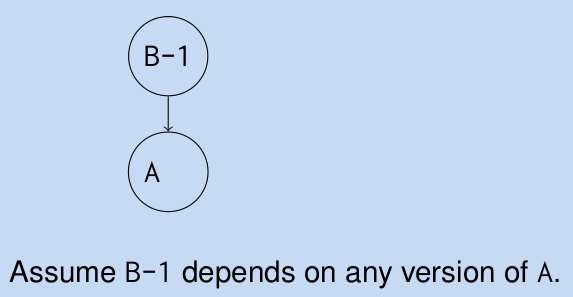
\includegraphics[height=5cm]{image201110/cabal-1.png}
  \end{center}
  \label{fig:cabal-1}\caption{Hackage DB上でB-1パッケージがAに依存している場合}
\end{figure}

まず上図のようにHackage DBでB-1パッケージがAパッケージに依存している場合を
考えます。この時B-1はAのバージョンについて特に指定していないとします。

\begin{figure}[ht]
  \begin{center}
    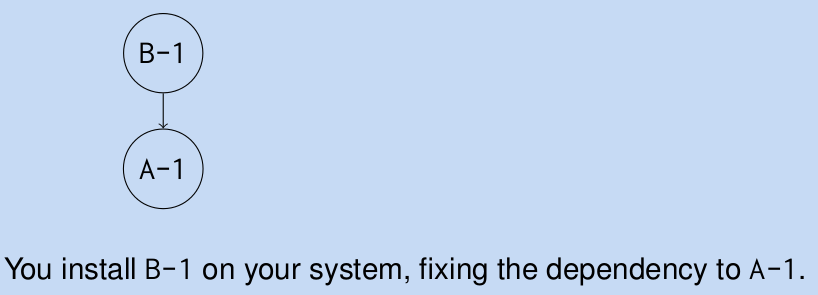
\includegraphics[height=5cm]{image201110/cabal-2.png}
  \end{center}
  \label{fig:cabal-2}\caption{B-1とA-1をインストール}
\end{figure}

このようなHackage DBからB-1をインストールするとAパッケージの最新バージョン
であるA-1も一緒にインストールされます。

\begin{figure}[ht]
  \begin{center}
    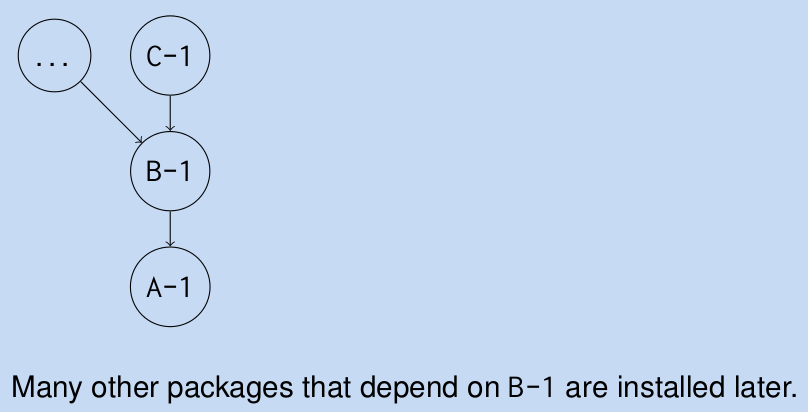
\includegraphics[height=5cm]{image201110/cabal-3.png}
  \end{center}
  \label{fig:cabal-3}\caption{そしてさらにB-1に依存したHackage群をインストール}
\end{figure}

そうして、このような環境にさらにC-1を含むB-1依存したHackage群をインストール
します。ここで、Bに依存しているC-1はローカルではB-1に紐づけられています。

\begin{figure}[ht]
  \begin{center}
    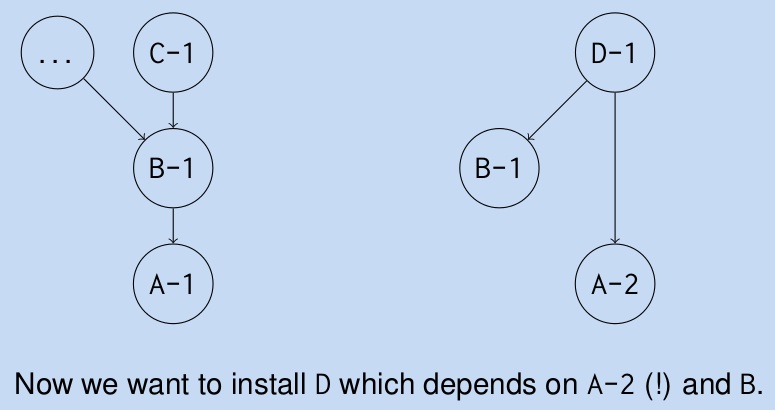
\includegraphics[height=5cm]{image201110/cabal-4.png}
  \end{center}
  \label{fig:cabal-4}\caption{A-2に依存しているD-1をインストールしようと試みる}
\end{figure}

ここでHackage DBからD-1をインストールしてみましょう。
D-1はHackage DB上(上図右)ではA-2とB-1にバージョン指定で依存しています。
ローカルにはA-1とB-1がインストールされています。

\begin{figure}[ht]
  \begin{center}
    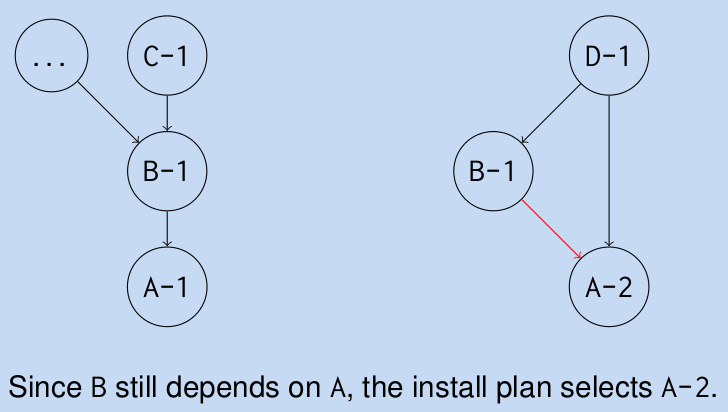
\includegraphics[height=5cm]{image201110/cabal-5.png}
  \end{center}
  \label{fig:cabal-5}\caption{cabalはD-1をインストールにあたってA-2もインストールしようとする}
\end{figure}

このままローカルにインストールされているA-1とB-1を無変更でD-1をインストール
することはできません。そこで、cabalはインストール計画をたて、
A-1のかわりにA-2をインストールしようとします。

\begin{figure}[ht]
  \begin{center}
    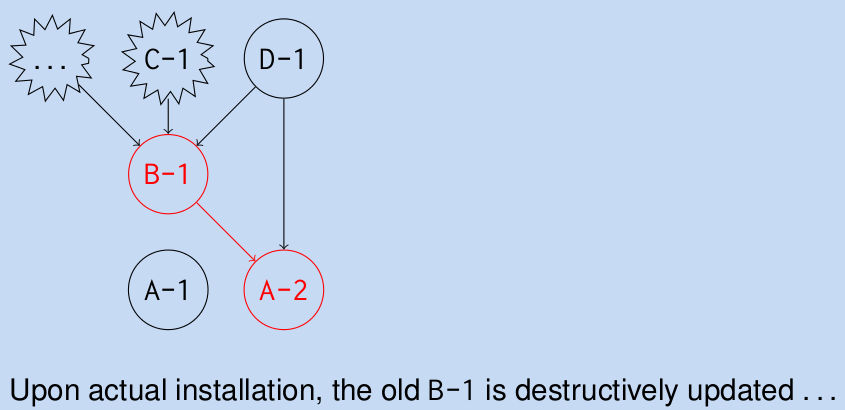
\includegraphics[height=5cm]{image201110/cabal-6.png}
  \end{center}
  \label{fig:cabal-6}\caption{D-1は正常にインストールされたが、B-1に依存していたHackage群は依存が壊れてしまう}
\end{figure}

A-2,B-1,D-1について\texttt{cabal}はインストール/更新を完了しました。
しかし、B-1に依存していたHackageについては再コンパイルは行ないません。
当然B-1に依存していたHackageは依存が壊れたまま放置されてしまうことになります。


この問題は依存解決する際のインストール計画の際にバックトラックが行なわれない
ためです。B-1を再インストールするのであれば、それに依存したHackage(C-1など)
も再インストールすべきだったのです。
もちろんHaskellコミュニティではこの問題を認識しており、その解決のために
新しいソルバを実装しています。
\footnote{\url{http://darcs.haskell.org/cabal-branches/cabal-modular-solver}}
近い将来に本家\texttt{cabal}に取り込まれることでしょう。

\subsubsection{Hackageが依存する環境についてcabalコマンドは面倒をみてくれない}

cairo
\footnote{\url{http://hackage.haskell.org/package/cairo}}
のようにC言語に依存するHackageについてはcabalコマンドは面倒を見てくれません。
Debianパッケージlibcairo2-devが入っていない環境で
cairo Hackageを\texttt{cabal}コマンドを使ってインストールしようとしても、
(当然)コンパイルエラーによってインストールに失敗します。

そもそもDebianではHaskell以外の部分のパッケージはDebianパッケージ(deb)によって管理されています。
cabalコマンドはOSに依存していないので、(当然)apt-getを呼び出すわけにもいきません。
\footnote{\url{http://packages.debian.org/ja/sid/auto-apt}
を使ってcabalコマンド実行の裏でDebianパッケージを自動インストールする手はあるかもしれませんね ;-)}

\subsubsection{Hackage群全てを最新バージョンでインストールできないかもしれない}

yesod \footnote{\url{http://hackage.haskell.org/package/yesod}}
,hakyll \footnote{\url{http://hackage.haskell.org/package/hakyll}}
,hamlet \footnote{\url{http://hackage.haskell.org/package/hamlet}}
の3つのHackageを例に説明します。
この問題はyesod-0.9.2, hakyll-3.2.0.8, hamlet-0.10.2のバージョン間で生じていました。(現在は解消されています)

まずそれぞれのHackageについて依存を見てみましょう。

\begin{commandline}
$ cabal info yesod-0.9.2
* yesod-0.9.2            (program and library)
--snip--
    Dependencies:  yesod-core >=0.9.1.1 && <0.10, yesod-auth ==0.7.*,
--snip--
                   hamlet ==0.10.*, shakespeare-js ==0.10.*,
--snip--
$ cabal info hakyll-3.2.0.8
* hakyll-3.2.0.8           (library)
--snip--
    Dependencies:  base ==4.*, binary >=0.5 && <1.0, blaze-html >=0.4 && <0.6,
--snip--
                   filepath >=1.0 && <2.0, hamlet >=0.7 && <0.9,
\end{commandline}

あれ?yesod-0.9.2はhamlet-0.10.*に依存しているのにhakyll-3.2.0.8は
hamlet-0.7.*もしくはhamlet-0.8.*に依存しています。
確かに表面上問題はありません。この状態でもyesodとhakyllの両方をインストール
することはできます。しかしもしhakyllとyesod両方のライブラリを使いたいプログラム
を作りたくなった場合にはどうしたら良いのでしょう?
hakyllはローカルでWebサーバを起動してプレビューする機能を持っています。
たまたまhakyllはこのWebサーバのエンジンとしてsnap
\footnote{\url{http://hackage.haskell.org/package/snap}}
を使っていたから良かったもののyesodを使っていたら、古いyesodの機能
しか使えないところです。

どうしてこんな状態でHackageが放置されていたのでしょう?
やる気がないのでしょうか?いえいえそんなことはありません。
今度はhamletについて調べてみましょう。

\begin{multicols}{2}
hamlet-0.8.2.1のModuleリスト
\begin{commandline}
Text
  Text.Cassius
  Text.Coffee
  Text.Hamlet
    Text.Hamlet.NonPoly
    Text.Hamlet.RT
  Text.Julius
  Text.Lucius
  Text.Romeo
  Text.Shakespeare
\end{commandline}
\columnbreak
hamlet-0.9.0のModuleリスト
\begin{commandline}
Text
  Text.Cassius
  Text.Coffee
  Text.Hamlet
  Text.Julius
  Text.Lucius
  Text.Romeo
  Text.Shakespeare
\end{commandline}
\end{multicols}

あれ?APIに変更があるようです。ここで注目したいのはText.Hamlet.RTモジュールが
消滅していることです。
嫌な予感がします。hakyllのソースコード
\footnote{\url{https://github.com/jaspervdj/hakyll/blob/master/src/Hakyll/Web/Template/Read/Hamlet.hs}}
を見てみましょう。

\begin{commandline}
-- | Read templates in the hamlet format
--
{-# LANGUAGE MultiParamTypeClasses #-}
module Hakyll.Web.Template.Read.Hamlet
    ( readHamletTemplate
    , readHamletTemplateWith
    ) where

import Text.Hamlet (HamletSettings, defaultHamletSettings)
import Text.Hamlet.RT

import Hakyll.Web.Template.Internal
--snip--
\end{commandline}

あーhakyllのコンパイルにはText.Hamlet.RTモジュールが必須なんですね。
これでは新しいhamletを使うことができない訳です。

Hackage作者が自由に依存Hackageのバージョンを選択可能である以上、
このようなHackage群全体の不整合は避けられません。

\subsection{HackageをDebianパッケージ化する}

cabalを使ってDebianパッケージと同等のレベルで
パッケージ管理をするのは現状では難しいことがわかりました。
それにapt-getでライブラリ環境が整うのはDebianユーザとしてうれしいですよね。
そこで、自分の良く使うHackageはDebianパッケージ化してDebian本体に
登録してしまうのはいかがでしょうか。
実はHackageをDebianパッケージ化するのはすごく簡単です。
\texttt{cabal-debian}というまんまの名前のコマンドがあります。\footnote{\url{http://hackage.haskell.org/package/debian}}
さっそくやってみましょう!

例題としてHCWiid
\footnote{Wiiリモコンからイベントを拾うためのライブラリ
  \url{http://hackage.haskell.org/package/hcwiid}}
をDebianパッケージ化してみます。
まずHackageのDebianパッケージ化に必要なhaskell-debian-utils,
haskell-devscriptsをapt-get installしましょう。

\begin{commandline}
$ sudo apt-get install haskell-debian-utils haskell-devscripts
$ rehash
\end{commandline}

hackageをダウンロードして解凍したら、ディレクトリに移動しておもむろに\texttt{cabal-debian}コマンドを使います。

\begin{commandline}
$ wget http://hackage.haskell.org/packages/archive/hcwiid/0.0.1/hcwiid-0.0.1.tar.gz
$ tar xfz hcwiid-0.0.1.tar.gz
$ cd hcwiid-0.0.1/
$ cabal-debian --debianize --ghc --maintainer="Kiwamu Okabe <kiwamu@debian.or.jp>"
$ ls debian
changelog  compat  control  copyright  rules*
$ debuild -rfakeroot -us -uc
--snip--
 dpkg-genchanges  >../haskell-hcwiid_0.0.1-1~hackage1_amd64.changes
dpkg-genchanges: including full source code in upload
 dpkg-source --after-build hcwiid-0.0.1
dpkg-buildpackage: full upload; Debian-native package (full source is included)
Now running lintian...
W: haskell-hcwiid source: native-package-with-dash-version
W: haskell-hcwiid source: out-of-date-standards-version 3.9.1 (current is 3.9.2)
E: libghc-hcwiid-dev: copyright-file-contains-full-gpl-license
E: libghc-hcwiid-dev: copyright-should-refer-to-common-license-file-for-lgpl
E: libghc-hcwiid-dev: description-contains-tabs
E: libghc-hcwiid-prof: copyright-file-contains-full-gpl-license
E: libghc-hcwiid-prof: copyright-should-refer-to-common-license-file-for-lgpl
E: libghc-hcwiid-prof: description-contains-tabs
E: libghc-hcwiid-doc: copyright-file-contains-full-gpl-license
E: libghc-hcwiid-doc: copyright-should-refer-to-common-license-file-for-lgpl
E: libghc-hcwiid-doc: description-contains-tabs
Finished running lintian.
$ ls ../*hcwiid*deb
../libghc-hcwiid-dev_0.0.1-1~hackage1_amd64.deb
../libghc-hcwiid-doc_0.0.1-1~hackage1_all.deb
../libghc-hcwiid-prof_0.0.1-1~hackage1_amd64.deb
\end{commandline}

なんかあっさりDebianパッケージができちゃいました。
lintianがなんか言ってますが、
あまり深刻なものではないのでとりあえずインストールしてみましょう。

\begin{commandline}
$ sudo dpkg -i ../libghc-hcwiid-dev_0.0.1-1\~hackage1_amd64.deb \
../libghc-hcwiid-doc_0.0.1-1\~hackage1_all.deb ../libghc-hcwiid-prof_0.0.1-1\~hackage1_amd64.deb
$ cd ~/
$ rm -rf .ghc .cabal # これでcabalでインストールしたパッケージは一切使っていないはずです
$ ghc-pkg list|grep hcwiid
    hcwiid-0.0.1
\end{commandline}
Hackageはインストール済みのようです。hcwiidライブラリを使ってみましょう。

Test.hs
\begin{commandline}
module Main where

import Prelude
import Control.Monad
import System.CWiid
import System.Posix.Unistd

main :: IO ()
main = do
  putStrLn "Put Wiimote in discoverable mode now (press 1+2)..."
  (Just wm) <- cwiidOpen
  putStrLn "found!"
  _ <- cwiidSetLed wm
  _ <- cwiidSetRptMode wm
  _ <- forever $ do _ <- usleep 300000
                    cwiidGetBtnState wm >>= print
  return () -- not reach
$ ghc --make Test.hs
[1 of 1] Compiling Main             ( Test.hs, Test.o )
Linking Test ...
$ ./Test
Put Wiimote in discoverable mode now (press 1+2)...
\end{commandline}

なんて簡単なんでしょう!簡単なHackageならcabal-debianコマンドを使えば
Debianパッケージ化が完了してしまうようです。
しかも下記3つのライブラリに分割してくれています。やった!

\begin{itemize}
 \item libghc-HOGE-dev  - 通常使用するライブラリ
 \item libghc-HOGE-doc  - Haddockで生成されたAPIドキュメント
 \item libghc-HOGE-prof - プロファイラ対応ライブラリ
\end{itemize}

\subsection{haskell-debian-utilsのしくみ}

cabal-debianでのDebianパッケージ化はどのようなしくみなのでしょうか。
さきほど作ったhcwiidパッケージのdebian/rulesファイルを見てみましょう。

\begin{commandline}
#!/usr/bin/make -f
include /usr/share/cdbs/1/rules/debhelper.mk
include /usr/share/cdbs/1/class/hlibrary.mk

# How to install an extra file into the documentation package
#binary-fixup/libghc-hcwiid-doc::
#       echo "Some informative text" > debian/libghc-hcwiid-doc/usr/share/doc/libghc-hcwiid-doc/AnExtraDocFile
\end{commandline}

なんということでしょう。内容がありません。。。
これはhlibrary.mkファイルに秘密があるに相違ありません。
全部を読まずにまずはlibghc-HOGE-devのbuildターゲットとその近辺をhlibrary.mk
から抜き出してみましょう。

\begin{commandline}
DEB_SETUP_BIN_NAME ?= debian/hlibrary.setup
BUILD_GHC := $(DEB_SETUP_BIN_NAME) build

$(DEB_SETUP_BIN_NAME):
        if test ! -e Setup.lhs -a ! -e Setup.hs; then echo "No setup script found!"; exit 1; fi
        for setup in Setup.lhs Setup.hs; do if test -e $$setup; then ghc --make $$setup -o $(DEB_SETUP_BIN_NAME); \
          exit 0; fi; done

build/libghc-$(CABAL_PACKAGE)-prof build/libghc-$(CABAL_PACKAGE)-dev:: build-ghc-stamp

build-ghc-stamp: dist-ghc
        $(BUILD_GHC) --builddir=dist-ghc
        touch build-ghc-stamp
\end{commandline}

なるほど。libghc-HOGE-devをbuildしようとすると、
まずSetup.lhsもしくはSetup.hsをghcを使ってコンパイルして\texttt{debian/hlibrary.setup}
コマンドを作成するようです。
そうして作ったdebian/hlibrary.setupコマンドを使って
"debian/hlibrary.setup build --builddir=dist-ghc"
のようにしてdist-ghcディレクトリ上でHackageをコンパイルするんですね。

ちょっと脱線しますが、
このビルドプロセスはcabalが普段やっていることと全く同じです。
cabalはインストール対象のHackageを取得/展開したら、まずこのSetup.hsを
ghcでコンパイルして、そのコンパイルした結果できた実行バイナリを
本当のビルダ/インストーラとして使います。
普段使っている/usr/bin/cabalコマンドは"cabal-install"と呼ばれています。
そして、Setup.hsを書くために必要なライブラリを"Cabal"と呼びます。
ややこしいですね。。。

ではlibghc-HOGE-devのinstallはどうなっているのでしょうか?

\begin{commandline}
debian/tmp-inst-ghc: $(DEB_SETUP_BIN_NAME) dist-ghc
	$(DEB_SETUP_BIN_NAME) copy --builddir=dist-ghc --destdir=debian/tmp-inst-ghc

install/libghc-$(CABAL_PACKAGE)-dev:: debian/tmp-inst-ghc debian/extra-depends
	cd debian/tmp-inst-ghc ; find usr/lib/haskell-packages/ghc/lib/ \
		\( ! -name "*_p.a" ! -name "*.p_hi" \) \
		-exec install -Dm 644 '{}' ../$(notdir $@)/'{}' ';'
	pkg_config=`$(DEB_SETUP_BIN_NAME) register --builddir=dist-ghc --gen-pkg-config | sed -r 's,.*: ,,'`; \
		$(if $(HASKELL_HIDE_PACKAGES),sed -i 's/^exposed: True$$/exposed: False/' $$pkg_config;) \
		install -Dm 644 $$pkg_config debian/$(notdir $@)/var/lib/ghc/package.conf.d/$$pkg_config; \
		rm -f $$pkg_config
	if [ 'z$(DEB_GHC_EXTRA_PACKAGES)' != 'z' ] ; then \
		echo '$(DEB_GHC_EXTRA_PACKAGES)' > \
                debian/$(notdir $@)/usr/lib/haskell-packages/ghc/lib/$(CABAL_PACKAGE)-$(CABAL_VERSION)/extra-packages ; \
	fi
	dh_haskell_provides -p$(notdir $@)
	dh_haskell_depends -p$(notdir $@)
	dh_haskell_shlibdeps -p$(notdir $@)
\end{commandline}

ちょっとわかりにくいですが、パッケージ化の後半はDebian流儀の詳細なので
踏みこまずに解釈すると、
まずlibghc-HOGE-devをinstallしようとすると、debian/tmp-inst-ghcターゲット
が呼び出されて
"debian/hlibrary.setup copy --builddir=dist-ghc --destdir=debian/tmp-inst-ghc"
のようなコマンドが実行されて、dist-ghcでコンパイルした内容が
debian/tmp-inst-ghc以下にインストールされます。
あとは、Debianの流儀にのっとってdebian/tmp-inst-ghc以下のファイル群を
パッケージ化するだけです。
パッケージ化対象のHackageが依存しているHackageも
dh\_haskell\_shlibdepsでちゃんと検出してくれるみたいです。 :)

\subsection{作ったパッケージをDebianに登録するには}

せっかく作ったHackageです。自分だけで使っているのはもったいないです。
Debian本家に登録して皆に使ってもらいましょう!
Debian本家に登録しておけばめぐりめぐってUbuntuにも登録されるかもしれませんよ?

%その秘技はプレゼン資料の方でこっそり、あなただけに、紹介します。 ;)

% 201110 kansai
\dancersection{Emacs, Vim の拡張機能で学ぶ Debian パッケージ}{西田孝三}
\index{emacs}
\index{vim}
\subsection{はじめに}

パッケージメンテナになることでDebianに関わりたいと思われている方は多いのではないでしょうか。
もしあなたがEmacs, Vimのユーザであればこれらの機能拡張でパッケージを作成するところから始めて
みるのはどうでしょうか。
理由は、
\begin{itemize}
 \item アーキテクチャに依存しない
 \item コンパイルは不要 (Emacsの場合バイトコンパイルがありますが)
\end{itemize}
などから比較的簡単と思われるためです。

ここでは大きく分けて下記のことを行い、まずは簡単なDebianパッケージを自分で作成できるようにな
るまでを目的としています。

\begin{itemize}
  \item EmacsのDebianパッケージ
    \begin{itemize}
      \item 既存のDebianパッケージの構成を知り再構成を行う
      \item 独自のDebianパッケージを作成する
    \end{itemize}
  \item VimのDebianパッケージ
    \begin{itemize}
      \item 既存のDebianパッケージの構成を知る
    \end{itemize}
\end{itemize}

Vimでは構成だけを学び、独自のDebianパッケージの作成を行いません。その理由は後に説明します。
それではEmacsの既存のDebianパッケージの構成を知り再構成を行うところから始めましょう。

\subsection{EmacsのDebianパッケージ}

\subsubsection{Emacsの既存Debianパッケージのソース取得と再構成}

ここでは前回の関西Debian勉強会で発表されていた山下尊也さんがメンテナンスをされている
auto-install-elのパッケージのソースを取得し、再構成を行います。

\begin{commandline}
 $ mkdir tmp; cd tmp
 $ apt-get source auto-install-el
 $ ls auto-install-el-1.48
\end{commandline}

これでtmpディレクトリ内にauto-install-elのソース(バージョン1.48)が取得できているはずです。
ソース内容を確認することは保留し、いきなりDebianパッケージを作ってみましょう。

\begin{commandline}
 $ cd auto-install-el-1.48
 $ debuild -us -uc
 $ ls ..
\end{commandline}

これでdebuildをしたディレクトリのひとつ上にauto-installのDebianパッケージができます。
それではこのDebianパッケージをインストールしてみましょう。

\begin{commandline}
 $ cd ..
 $ sudo dpkg -i auto-instlal-el_1.48-1_all.deb
 $ aptitude show auto-install-el
\end{commandline}

これでauto-install-elがインストールされたことがわかります。
それではうまく使えるかどうかEmacsで確認してみましょう。

\begin{commandline}
 $ emacs -nw
 M-x load-library
 auto-install
 auto-install-from-emacswiki
 grep-edit.el
\end{commandline}

これで ~/.emacs.d/auto-install/ 下にgrep-edit.el(elc)がインストールされていることが
確認できます。

それでは保留していたソースの構成の確認に戻りましょう。
が、その前にもう一つ別のディレクトリにauto-install-elのソースを取得しましょう。
というのはdebuild後にはいくつかのファイルが生成されているからです。
2つのソースディレクトリを比較することでこれらのファイルが確認できます。
詳細はご自身でご確認ください。

\begin{commandline}
 $ cd; mkdir auto-install-el
 $ cd auto-install-el; apt-get source auto-install-el
\end{commandline}

それではdebuildする前のauto-install-el-1.48内のファイル構成を見てみましょう。
auto-install.elというファイルとdebianというディレクトリがあります。
このことからEmacsの拡張機能のDebianパッケージを作るには

\begin{itemize}
 \item Emacsの拡張機能にバージョン名を加えた名前のディレクトリを作り
 \item その下にEmacs Lispとdebianというディレクトリを作ればよい
\end{itemize}

ということがわかります。それではこれをまだDebianパッケージが作られていないEmacs
の拡張機能に対して行っていきましょう。

\subsubsection{Emacsの新規Debianパッケージの作成}

今回は青田直大さんによるtwinstall.elのパッケージを作ってみましょう。
これはtwittering-modeというEmacs用twitterクライアントの機能を使って、
auto-install.elでインストールしたEmacs Lisp名をつぶやくものです。
現時点ではIDが1300477のgist(https://gist.github.com/1300477)から取得できます。

\begin{commandline}
 $ tar zxvf gist1300477.tar.gz
 $ mv gist1300477 twinstall-el-0.1
 $ tar czvf twinstall-el-0.1.tar.gz twinstall-el-0.1
 $ cd twinstall-el-0.1
 $ cat >>~/.bashrc <<EOF
  DEBEMAIL=''your.email.address@example.org''
  DEBFULLNAME=''Firstname Lastname''
  export DEBEMAIL DEBFULLNAME
  EOF
 $ . ~/.bashrc
 $ dh_make -f ../twinstall-el-0.1.tar.gz
\end{commandline}

次にどのような種類のパッケージを作るか聞かれるのでsingleのsにしenterを押します。
するとdebianディレクトリとその下に各種設定ファイルの雛形が生成されます。
多くのファイルができあがりますが、auto-install-elと同じものがあればよいので対応す
るファイルは削除し、後はauto-install-elを真似てファイル内容を変更していきましょう。
(変更せずにこの段階でdebuildを行っても一応パッケージはできます。)
それでは各ファイルの説明をします。

\clearpage

\paragraph{\texttt{README.Debian}}
  \begin{itemize}
    \item DebianパッケージのREADME
    \item 必須ではない?
  \end{itemize}

\paragraph{\texttt{changelog}}
  \begin{itemize}
    \item 必須のファイル
    \item Debianのポリシーで規定された書式
  \end{itemize}

\paragraph{\texttt{compat}}
  \begin{itemize}
    \item わかりませんでした!
    \item 作られた雛形のままにしましょう
  \end{itemize}

\paragraph{\texttt{control}}
  \begin{itemize}
    \item 必須のファイル
    \item aptitudeなどのパッケージ管理ツールが利用する情報
    \item Debianのポリシーで規定された書式
    \item twinstall.elはauto-installとtwittering-modeに依存している。Depends:に追加
  \end{itemize}

\paragraph{\texttt{copyright}}
  \begin{itemize}
    \item 必須のファイル
    \item upstreamソースに関する著作権やライセンスなどの情報を書く
    \item Debianのポリシーで規定された書式
  \end{itemize}

\paragraph{\texttt{dirs}}
  \begin{itemize}
    \item ファイルをインストールするディレクトリを書く
    \item 前述ディレクトリのパスのトップの/は書かない
  \end{itemize}

\paragraph{\texttt{emacsen-install, emacsen-remove}}
  \begin{itemize}
    \item install, uninstall時に行う処理をやってくれるシェルスクリプト
  \end{itemize}

\paragraph{\texttt{emacsen-startup}}
  \begin{itemize}
    \item elispのインストールディレクトリにdirsで書いたインストール先をEmacsのload-pathに追加してくれるelisp
    \item これ自体は/etc/emacs/site-start.d/に50'パッケージ名'.elという名でインストールされる
  \end{itemize}

\paragraph{\texttt{rules}}
  \begin{itemize}
    \item 必須のファイル
    \item パッケージを作成するために使うルールを書く
    \item まずはとりあえず人様のものを真似る
  \end{itemize}

\paragraph{\texttt{source}}
  \begin{itemize}
    \item わかりませんでした!
    \item 作られた雛形のままにしましょう
  \end{itemize}

\begin{commandline}
 $ debuild -us -uc
 $ cd ..
 $ sudo dpkg -i twinstall-el_0.1-1_all.deb
\end{commandline}

controlのDepends以外はauto-install-elを真似て新規パッケージに応じた情報に置き換えることでtwinstallのDebianパッケージが出来ます。
後はこのDebianパッケージを公開する必要があるかを考え、ライセンスなどを学び、公開に必要な次のステップへ進んでください。
もちろんコンパイルが必要なパッケージ作成へとレベルアップするのもよいでしょう。

\subsection{Vimの既存パッケージのソース取得}

Vimの拡張機能のDebianパッケージはEmacsと比較すると数は少なく、あまりパッケージを作るモチベーションが得られなさそうです。
そのためVimに関してはパッケージ作成までは行いません。
実際にRails用のVim scriptパッケージのソースを取得しその内容をみてみましょう。

\begin{commandline}
 $ apt-get source vim-rails
\end{commandline}

これで取得できるソースのREADME.Debianとcontrolを見るとvim-addon-managerというパッケージを使いvim-addonsというコマンドで
vim-railsを使用可能にするということを行なっていることがわかります。
これではDebianのパッケージマネージャーとVimのaddon-managerでmanagerを2つ用いていることになり、あまり良いこととは思えません。
現在のVimユーザの多くはvim-addon-managerよりbundleやneobundleといったVim scriptで書かれたmanagerを用いており、これらの完成
度が高いためDebianのパッケージは不要なのかもしれません。

% 201110 tokyo
%-------------------------------------------------------------------------------
\dancersection{月刊 debhelper 第1回}{岩松 信洋}
%-------------------------------------------------------------------------------
\index{debhelper}

\subsection{debhelper とは何か?}

Debian パッケージを作成する時、パッケージに必要なファイルのチェック、
コンパイル前の設定、コンパイルなど様々な処理を行う必要があります。
Debianパッケージでは debian/rules という GNU Make のmakefile に各処理
を記述するのですが、細かい処理をひとつづつ書いていくと膨大な量になります。

またコードの量が多くなるとバグも多くなり、パッケージ作成時に問題が起きた
ときに修正するのは大変です。
これらの処理を機能毎にまとめ、使いやすくした機能を提供しているパッケージ
として debhelper があります。他にも同様のツールがいくつかありますが、
1番使われているのがこの debhelper です。
Debian パッケージをメンテナンスしている人にとって debhelper の知識が必須と
言ってもいいでしょう。

ちなみにdebhelper は Debian 開発者の Joey Hess 氏\footnote{Wikiエンジンのikiwiki,
ディストリビューションのパッケージ間変換ツールである alien の開発者として有名。}
によって開発/メンテナンスされ、最新のバージョンは 8.9.8 となっています。

\subsection{月刊 debhelperとは?}
先にも説明したように、Debian パッケージをメンテナンスしている人にとって
debhelper の知識が必須となっています。
debhelper がどのような機能を提供して、それらをどのように使えばいいのか、
どのように使われているのか、理解しておく必要があります。
現時点で debhelper では59個のコマンド(dh\_で始まるコマンド)が提供されており、
全部理解するのは難しいでしょう。また、debhelper に収録されていない debhelper サポートツール
を含めると100個ほどになります。
日頃Debianの開発を行なっている人でも「ああ、こんな機能があるのだ」と思うことがあるぐらいです。
更にdebhelper 7 からコマンドがいくつか増え、debian/rules ファイルが以下のように記述
できるようになりました。

これだけでは何をやっているのかさっぱり分かりません。
細かい指定を行いたい場合、どのようにしたらいいのかすらわからない状態です。

そこで debhelper で提供されているコマンドの動きと使い方を毎月数個づつ
紹介し、Debian勉強会参加者でパッケージ作成の理解を深める企画、「月刊 debhelper」
を企画しました。
全て理解した頃には、皆 Debian パッケージメンテナになっているかもしれません。
ヒャッハー!

\begin{multicols}{2}

\begin{commandline}
debhelper 6:
#!/usr/bin/make -f

build: build-stamp
build-stamp:
    dh_testdir
    $(MAKE)
    touch $@

clean:
    dh_testdir
    dh_testroot
    $(MAKE) clean
    dh_clean

install: build
    dh_testdir
    dh_testroot
    dh_clean -k

binary-indep:

binary-arch: build install
    dh_testdir
    dh_testroot
    dh_installchangelogs ChangeLog
    dh_installd
.....
\end{commandline}
\columnbreak
\begin{commandline}
debhelper 7:
#!/usr/bin/make -f
%:
        dh $@
\end{commandline}
\end{multicols}
% $

\subsection{debian パッケージ構築、全体の流れ}

いきなり個々のコマンド説明をしてもよくわからないので、パッケージ作成の全体の
流れとどのようなコマンドが呼び出されるのか説明します。
Debian パッケージが作成される簡単流れは以下の通りで、
図にすると図\ref{fig:rules-work}のようになります。

\begin{enumerate}
\item パッケージビルド環境を構築する

実際にビルドを始める前に、まずはビルドのための環境を構築する必要があります。
ここでは、ソースコードの展開、パッケージ構築依存のチェック等を行います。

\item 不要なファイルを削除する\\
次にパッケージに不要なファイルを削除します。
例えば、前に行われたパッケージビルドで生成されたファイルがある場合はそれを削除して、
ソースが展開された常に同じ状態からビルドできるようにします。

これは debian/rules ファイルの {\bf clean} ターゲットで行われ、このターゲットは
「不要なファイルを削除する」ことを目的とするように Debian Policy で定められています。

また clean ターゲットでは、以下の dehhelper コマンドが実行されます。
\begin{commandline}
dh_testdir -> dh_auto_clean -> dh_clean
\end{commandline}

\item  バイナリパッケージに格納するファイルをビルドする

次にソースコードからバイナリをビルドします。ここではconfigure などを使った
コンパイル前の設定、コンパイラを使った実行ファイルの作成、ドキュメントの変
換などがおこなわれます。

これは debian/rules ファイルの {\bf build} ターゲットで行われ、このターゲットは
「プログラムの設定、コンパイルやデータの変換」ことを目的とするように Debian Policy で
定められています。

また build ターゲットでは、以下の dehhelper コマンドが実行されます。
\begin{commandline}
dh_testdir -> dh_auto_configure -> dh_auto_build -> dh_auto_test
\end{commandline}

\item ビルドしたファイルをバイナリパッケージにまとめる

必要なファイルをすべてビルド完了した後、それらを適切なパーミッションで
適切な場所に配置し、バイナリパッケージにまとめます。

ここでは、debian/tmpを/(ルート)と見なしてソフトウェア全体の
インストール (「仮インストール」) を行い、 その上でdebian/tmp 内の各ファイルを適切に
debian/バイナリパッケージ名に振り分け、 最後にdebian/バイナリパッケージ名をそれぞれ
バイナリパッケージ化する、という流れで行います。 debian/バイナリパッケージ名 を
バイナリパッケージ化する際には、各ファイルのパーミッションの設定やファイルの圧縮など、
行わなければならないことや、推奨されていることが多数あります。

これは debian/rules ファイルの {\bf binary、binary-arch、 binary-indep}
ターゲットで行われ、このターゲットは
「バイナリパッケージとしてまとめる」ことを目的とするように Debian Policy で
定められています。

また binary、binary-arch、 binary-indep ターゲットでは、以下の dehhelper コマンドが実行されます。
\begin{commandline}
dh_testdir -> dh_auto_configure -> dh_auto_build -> dh_auto_test -> dh_testroot
-> dh_prep -> dh_installdirs -> dh_auto_install -> dh_install -> dh_installdocs
-> dh_installchangelogs -> dh_installexamples -> dh_installman -> dh_installcatalogs
-> dh_installcron -> dh_installdebconf -> dh_installemacsen -> dh_installifupdown
-> dh_installinfo -> dh_pysupport -> dh_installinit -> dh_installmenu -> dh_installmime
-> dh_installmodules -> dh_installlogcheck -> dh_installlogrotate -> dh_installpam
-> dh_installppp -> dh_installudev -> dh_installwm -> dh_installxfonts -> dh_installgsettings
-> dh_bugfiles -> dh_ucf -> dh_lintian -> dh_gconf -> dh_icons -> dh_perl -> dh_usrlocal
-> dh_link -> dh_compress -> dh_fixperms -> dh_strip -> dh_makeshlibs -> dh_shlibdeps
-> dh_installdeb -> dh_gencontrol -> dh_md5sums -> dh_builddeb
\end{commandline}

\item .changesファイルを作成する

パッケージが作成されたら、そのパッケージの.changelog ファイルを作成します。
このファイルの作成には dpkg-genchanges コマンドが使われます。
このコマンドは debhelper のコマンドではありません。
\item パッケージに署名する

必須ではありませんが、パッケージができたら.dscファイルと.changes ファイルに
GPG/PGPを使って署名をします。この署名には debsign コマンドを使います。
このコマンドは debhelper のコマンドではありません。
\end{enumerate}

\begin{figure}[ht]
  \begin{center}
    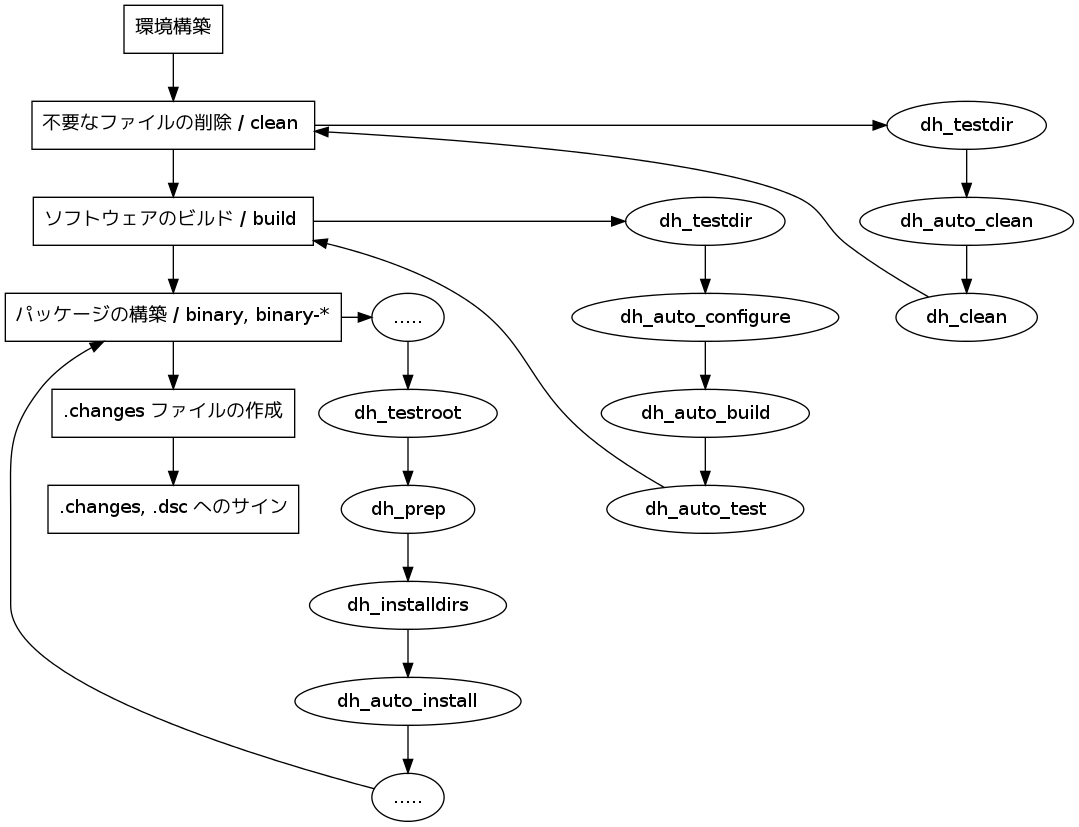
\includegraphics[height=10cm]{image201110/rules-work.png}
  \end{center}
  \label{fig:rules-work}\caption{各処理とdebhelperコマンドの関係図}
\end{figure}

\subsection{その他 debhelper の重要な機能}

\subsubsection{環境にあわせたシーケンス情報を読み込む}
debhelper は特定の言語や環境に合わせたシーケンスを定義し、
読み込ませることによって、makefile 内で利用できるターゲットとコマンドを増やすことができます。
例えば、パッチ管理ツールである quilt を使ったターゲットは debhelper には含まれていません。
使いたい場合には、{\bf --with}オプションを使って指定します。

\begin{commandline}
%:
        dh $@ --with quilt
\end{commandline}
%$
指定することによって、{\bf{dh\_quilt\_patch}}が利用できるようになります。

\subsubsection{各 debhelper コマンドの動きを変更する}
上記で説明しように、debhelper では各ターゲットと各コマンドの動作が予め決められています。
これらを変更するには各コマンド用のターゲットに対して動作を記述します。
このターゲットは {\bf override\_各debhelper コマンド}となっており、dh\_auto\_configure
(決められた値で自動的に configure を実行するためのコマンド)の場合には以下のように使います。

\begin{commandline}
override_dh_auto_configure:
    dh_auto_configure -- --enable-foo
\end{commandline}

\subsection{今月のコマンド : dh\_testdir}

\subsubsection{概要}

パッケージビルドを行うときに正しいディレクトリにいるかチェックします。

\subsubsection{使い方}

dh\_testdir コマンドはカレントディレクトリに debian/control があることに
よって正しいディレクトリにいるかチェックをしています。
dh\_testdir はほとんどのターゲットから利用されます。ちゃんと debian パッケージ
をビルドできる場所にいるかチェックするためです。


\begin{commandline}
$ mkdir foo
$ cd foo
$ dh_testdir
dh_testdir: cannot read debian/control: そのようなファイルやディレクトリはありません
echo $?
2
$ mkdir debian
$ touch debian/control
$ dh_testdir
$ echo $?
0
\end{commandline}
%$

引数としてファイルパスを指定することができます。
ファイルパスを指定した場合には、指定したファイルによってチェックが行われます。

\begin{commandline}
$ touch moo
$ dh_testdir moo
$ echo $?
0
\end{commandline}
%$

\subsection{今月のコマンド : dh\_bugfiles}

\subsubsection{概要}

dh\_bugfiles コマンドは バグレポートに必要なファイルをパッケージに
格納します。
バグレポートに使うファイルは script、control、presubj の3つがあり、
debian/bug ディレクトリに格納されている必要があります。
各ファイルの用途を以下に説明します。

\begin{itemize}
\item script

バグレポート用のスクリプトです。
バグレポートを行うためのツールreportbugs 等でレポート作成時に呼び出し、
結果をバグレポートの一部として追記します。
例えば、X.Orgのドライバ群は /usr/share/bug/xserver-xorg-core/script
にシンボリックリングを張ったファイルをバイナリパッケージ内に持ちます。
このスクリプトでは、reportbug を実行した環境のカーネルバージョンや
dmesg, xorg のログなどが自動的に出力されるようになっています。

\item control

controlファイルは指定したコマンドの結果をバグレポートの一部として出力します。
コマンドには以下の4つがあります。

\begin{itemize}
\item package-status
指定したパッケージのステータス(インストール状態、バージョン)を
バグレポートに追加します。

\begin{commandline}
設定例:
/usr/share/bug/mutt/control package-status: mutt mutt-patched mutt-dbg
\end{commandline}

\item report-with
指定したパッケージ情報をバグレポートに追加します。

\begin{commandline}
設定例:
/usr/share/bug/xorg/control report-with: xserver-xorg
\end{commandline}

\item Send-To
Debian BTS以外に自動的にが行われるメールアドレスを設定します。

\begin{commandline}
Send-To: foo@example.org
\end{commandline}

\item Submit-As:
一つのパッケージにレポートが行われるようにコントールする
以下のように設定した場合、linux-image-3.0.0-2-amd64 にバグレポート
した場合には linux-2.6 に行われるように自動的に変更されます。

\begin{commandline}
control:Submit-As: linux-2.6
\end{commandline}
\end{itemize}

\item presubj

レポートする前の警告文を出すために使います。
例えば、gnupg パッケージの場合にはこのファイルに
\begin{commandline}
Please consider reading /usr/share/doc/gnupg/README.BUGS.Debian before
sending a bug report. Maybe you'll find your problem there.
\end{commandline}
と書くことによって、バグレポートを送る前に /usr/share/doc/gnupg/README.BUGS.Debian
を参照するよう、誘導しています。

reportbug を使って、gnupg パッケージにバグレポートしようとしたとき、以下のような
メッセージが表示されます。
\begin{commandline}
Please consider reading /usr/share/doc/gnupg/README.BUGS.Debian before
sending a bug report. Maybe you'll find your problem there.


(You may need to press 'q' to exit your pager and continue using
reportbug at this point.)
\end{commandline}

\end{itemize}

これらのファイルは一つだけでもかまいません。

\subsubsection{使い方}

このコマンドは install ターゲットで使用します。

\begin{commandline}
install:
    ....
    dh_bugfiles
    ....
\end{commandline}

%\subsection{次の発表者}
%次の発表者は 勉強会で発表します。選ばれた人、おめでとうございます。
%頑張ってください。

% 201108 tokyo
%------------------------------------------------------------------------------
\dancersection{aufsbuilder - cowbuilderにたたかいをいどむ}{やまだ}
%------------------------------------------------------------------------------
\index{aufsbuilder}
\index{cowbuilder}

\subsection{やってみた}
数年前にaufsがマイブームだった時、
\begin{quote}
\Large{これでaufsbuilder書いたらcowbuilerに勝てるんじゃね?}
\end{quote}
と思ってやってみたものの、僅差ながら負けてお蔵入りしていた
aufsbuilderがこのほど勝利したので報告します。

\subsection{つくりかた}
実は pbuilder は chroot 環境に任意の場所を指定することができ、

\begin{commandline}
pbuilder $PBCMD --no-targz --buildplace <適当なchroot先>
\end{commandline}

と呼び出してやるだけで、よろしくビルドしてくれます。なので、
これを呼び出す前にテンプレート用chroot環境に書き込み用使い捨て
フォルダをラップしたaufs chrootを作ってやればいいわけです。

%以下コード:
\begin{commandline}
#!/bin/sh -e

: ${PB_BASE=/var/cache/pbuilder}
: ${PB_WORK=/var/cache/pbuilder/build}

usage() {
  P=$(basename $0)
  test $# -gt 0 && echo $@ >&2
  cat <<EOF 1>&2
$P - pbuilder wrapper with aufs-wrapped chroot
Usage: $P ...pbuilder-args...
Note:
- You need to define PB_BASE and PB_WORK
- For base chroot tree, \$PB_BASE/\$ARCH-\$DIST.cow/ will be used.
- For actual work tree, \$PB_WORK/\$\$/ will be used.
- Default: PB_BASE=$PB_BASE, PB_WORK=$PB_WORK
EOF
  exit 1
}

# pass all args to pbuilder (0 args == help)
test $# -gt 0 || usage
test $# -gt 0 && PBCMD="$1"; shift
test $# -gt 0 && PBARG="$@"

# prepare env
: ${DIST:=sid}
: ${ARCH:=$(dpkg-architecture -qDEB_HOST_ARCH)}
export ARCH DIST

MT="$PB_WORK/$$"
RW="$PB_WORK/$$/rw"
AD="$PB_BASE/$DIST-$ARCH"
RO="$PB_BASE/$DIST-$ARCH.cow"
\end{commandline}
\begin{commandline}
# sanity check
test -d "$MT" && usage "ERROR: Workdir already exists: $MT"
test -d "$RW" && usage "ERROR: Workdir already exists: $RW"
test -d "$RO" || usage "ERROR: Missing template: $RO"

# register cleanup hook
trap "
$DEBUG umount -lf '$MT/var/cache/apt' '$MT' && $DEBUG rm -fr '$MT'
" 0 1 2 3 4 6 7 8 11 15

# prepare chroot tree
$DEBUG mkdir -p "$RW" "$AD/aptcache"
$DEBUG mount -t aufs -o "br:$RW:$RO=ro" none "$MT"
$DEBUG mount --rbind "$AD/aptcache" "$MT/var/cache/apt"

# run pbuilder
$DEBUG pbuilder $PBCMD --aptcache "" --no-targz --buildplace "$MT" "$@"
\end{commandline}

\subsection{たたかってみる}

pbuilderとcowbuilderの関係同様、aufsbuilderもpbuilder互換なので
そのまま

\begin{commandline}
$ PDEBUILD_PBUILDER=aufsbuilder \
git-buildpackage --git-builder=''pdebuild --buildresult ..''
\end{commandline}

としてビルドするだけです。では、比較してみましょう。

まずは素のpbuilder:
\begin{commandline}
$ sudo rm ../cocot_20100903-1*
$ time sudo ARCH=i386 DIST=sid \
git-buildpackage --git-builder=''pdebuild --buildresult ..''
$ time sudo ARCH=i386 DIST=sid \
git-buildpackage --git-builder=''pdebuild --buildresult ..''
    0m44.76s real     0m21.50s user     0m13.62s system
\end{commandline}

続いてcowbuilder:
\begin{commandline}
$ sudo rm ../cocot_20100903-1*
$ time sudo ARCH=i386 DIST=sid PDEBUILD_PBUILDER=cowbuilder \
git-buildpackage --git-builder=''pdebuild --buildresult ..''
$ time sudo ARCH=i386 DIST=sid PDEBUILD_PBUILDER=cowbuilder \
git-buildpackage --git-builder=''pdebuild --buildresult ..''
    0m33.17s real     0m20.42s user     0m8.84s system
\end{commandline}

そしてaufsbuilder:
\begin{commandline}
$ sudo rm ../cocot_20100903-1*
$ time sudo ARCH=i386 DIST=sid PDEBUILD_PBUILDER=aufsbuilder \
git-buildpackage --git-builder=''pdebuild --buildresult ..''
$ time sudo ARCH=i386 DIST=sid PDEBUILD_PBUILDER=aufsbuilder \
git-buildpackage --git-builder=''pdebuild --buildresult ..''
    0m29.41s real     0m18.46s user     0m8.17s system
\end{commandline}

前回は何回やっても数秒差で負け続けたので、逆転できて嬉しい。
たぶんLKMLの小人さん達が頑張ってくれたおかげmOm

\subsection{まとめ}
aufsを使ったcowbuilderを作ってみました。
以前作った時はどうやっても勝てなかったのに、いつのまにか
速くなっていて嬉しい。

\subsection{だがしかし・・・}
\begin{commandline}
$ sudo rm ../cocot_20100903-1*
$ debuild --no-lintian -us -uc -Tclean
$ time git-buildpackage --git-builder=''DEB_CFLAGS_APPEND=-m32 debuild -ai386''
$ time git-buildpackage --git-builder=''DEB_CFLAGS_APPEND=-m32 debuild -ai386''
    0m13.95s real     0m12.17s user     0m4.74s system
\end{commandline}
ネイティブビルド、やっぱり速い。しかもlintianとdebsign時間まで入ってるし。

% 201106 kansai
%-------------------------------------------------------------------------------
\dancersection{vcs-buildpackage $\sim$Git、svn編$\sim$}{佐々木 洋平}
%-------------------------------------------------------------------------------

\subsection{始めに}

今日のお題は、
パッケージ作成に Git や Subversion を使用するソフトウェアである、
{\tt{git-buildpackage}}と{\tt{svn-buildpackage}}です。
自分の抱えている野良パッケージの多くが Ruby 関連だったこともあって、
PkgRubyExtras に参加したところ、
パッケージ管理を Subversion から Git へ移行するタイミングだった様で、
(幸か不幸か)両 VCS を使用してのパッケージ作成を体験しました%
\footnote{自分一人だったら絶対 Git で作業するんですけれどね}。

そこで覚えたツールの使い方とか、実際に作業する際のハマり所とかについて簡単に紹介できたら良いな、とか思います。
とはいえ、実際にはコラボする人々(=チーム)毎に work flow があるので、あまり一般論は言えない訳ですけれど。

\subsection{バージョン管理?}

バージョン管理システム(VCS)についてはほとんど説明しませんが、簡単に。

VCS を使った事のない人に VCS の利点を説明する時、佐々木は良く「良い感じのバックアップ」という言い方をしています。
例えば
\begin{itemize}
\item 過去の変更履歴を残しておける
\item 過去の任意の状態に簡単に戻せる
\item 過去にどんな変更を行なったか、を把握しやすくする(ログをきちんと書いておく必要はありますが)
\end{itemize}

また、複数人で開発を進めている時には、同じファイルに同じ様な変更を加えている場合、
最後に保存した人の変更だけが残ってしまい(上書きされてしまい)、それ以外の変更が失なわれてしまいます。
VCS を使っていると、同じファイルへの変更は「衝突」として検出されるので、こういった事態を防ぐ事ができます。

さらに、特定のバージョンに名前をつけておき(tag と言います)そのバージョンへの変更を行なったり、新機能の開発を本番の開発と分離して進めて(本番が main line と呼ばれるのに対して、branch を分ける、branch を切る、と言います)、完成した後で本番の開発に統合したりできます。

Subversion と Git は、それぞれ「集中型VCS」と「分散型VCS」の代表です。
集中型 VCS では単一のリポジトリ(データ置き場)を開発者全員が参照し作業するのに対して、
分散型 VCS では、各人が個別にリポジトリを持ち、各々のデータを適宜同期を取って作業を進めます。
最近は分散型 VCS(DVCS と言ったりします)がトレンドですね%
\footnote{集中型VCS としては CVS なんかもありますが、今更 CVS ってのは止めた方が良いと思います。また DVCS としたは Git 以外に darcs, bzr, Mercurial なんかがあります。bzr についてはそのうち山下 尊也さんが語ってくれると思います}。

\subsection{パッケージのバージョン管理?}

さて、「パッケージのバージョン管理」って何をしているのでしょうか?
Debian パッケージを「バージョン管理」する目的は幾つかありますが、
例えば
\begin{itemize}
\item 履歴の管理。
  パッケージの変更点は debian/changelog に書かれます(書きます)が、
  実際にファイル自体を参照できると大変便利です。
\item stable に含まれたパッケージにタグを付けておく。
  \begin{itemize}
  \item セキュリティ対応などを、そのタグから派生するブランチで対応する
  \end{itemize}
\item 複数人でのパッケージメンテ/チームでのパッケージメンテ作業の環境を容易に構築できる
\item upstream が VCS を使用している場合の連携が簡単になる(かも)
\end{itemize}
...でしょうか。

\subsection{何を管理するの?}
Debian のソースパッケージは、source format 3.0 では以下のファイル群で構成されます:
\begin{description}
\item[.orig.tar.{\it{ext}}] \\
  upstream のソース。複数のソースからなる場合には基本となるソースにこの名
  前をつける。{\it{ext}}は圧縮の拡張子であ
  り、{\tt{gz}}, {\tt{bz2}}, {\tt{xz}} が使用可能。
\item[.orig-{\it{component}}.tar.{\it{ext}}]  \\
  upstream が複数のソースから構成される場合のファイル
  名。{\tt{dpkg-source -x パッケージ名.dsc}}などで展開するとファイルの中
  身は {\tt{component/}}以下の展開される。
\item[.debian.tar.{\it{ext}}] \\
  {\tt{debian/}} デイレクトリの中身
\item[.dsc] \\
  パッケージの情報。上記ファイル群のハッシュなどを記載している。
\end{description}
パッケージを VCS で管理する場合、
\begin{enumerate}
\item {\tt{.orig.tar.{\it{ext}}}}
\item {\tt{.debian.tar.{\it{ext}}}}
\end{enumerate}
のバージョンを管理することになります。

\subsection{どうするの?: svn-buildpackage 編}
\index{svn-buildpackage}

では実際にどうやっているのでしょうか?
ここでは GNU Hello を例に、svn-buildpackage を使った場合について簡単に述べてみます。
なお、佐々木は既に svn-buildpackage をあまり使っていないので、
Git はまだ良くわからないけれど Subversion ならわかる、 という人向けのお話です。

\subsubsection{インストール}
\begin{commandline}
 $ sudo aptitude install svn-buildpackage
\end{commandline}

\subsubsection{パッケージをリポジトリに追加する}

一度適当なパッケージを作成してみましょう。 ここでは GNU hello のパッケージが作成できたとします。
横着したい人は{\tt{apt-get source hello}}でも良いでしょう。

テストのために簡単なリポジトリを作成します。ここでは {\tt{~/Work/svn/}} 以下にリポジトリを作成します。
\begin{commandline}
 $ svnadmin create ~/Work/svn/
 $ svn mkdir file:///home/uwabami/Work/svn/trunk -m "create trunk"
 $ svn mkdir file:///home/uwabami/Work/svn/tags -m "create tags"
 $ svn mkdir file:///home/uwabami/Work/svn/branches -m "create branches"
 $ svn ls file:///home/uwabami/Work/svn
  branches/
  tags/
  trunk/
\end{commandline}
次に、作成したパッケージをリポジトリに追加します。追加するコマンドは {\tt{svn-inject}} です。
\begin{commandline}
 $ svn-inject -l 2 -o -c 0 hello_2.7-1.dsc file:///home/uwabami/Work/svn
\end{commandline}
svn-inject のオプションの詳細は man を見てもらうとして、ここでは
\begin{commandline}
      -l
          Layout type.
          1 (default) means package/{trunk,tags,branches,...} scheme,
          2 means the {trunk,tags,branches,...}/package scheme.
      -o
          Only keep modified files under SVN control (including the debian/ directory),
          track only parts of upstream branch

       -c number
          Checkout nothing (0), trunk directory (1) or everything (2) when
          the work is done.
\end{commandline}
を用いています. 単一のパッケージを単一のリポジトリで管理する場合には {\tt{-l 1}} が良いでしょう.

\subsubsection{パッケージのビルド}

{\tt{svn-inject}}が終わったので、リポジトリからファイルを取得してみます。
\begin{commandline}
 $ svn checkout file:///home/uwabami/Work/svn/trunk svn-work
  A    trunk/hello
  A    trunk/hello/debian
  A    trunk/hello/debian/control
  A    trunk/hello/debian/source
  A    trunk/hello/debian/source/format
  ...
\end{commandline}
ここでは {\tt{svn-work}} にファイルをチェックアウトしました。
実際に {\tt{svn-work/trunk/hello}} に移動して、パッケージを作成してみます。
\begin{commandline}
 $ cd svn-work/trunk/hello
 $ sudo apt-get build-dep hello
 $ svn-buildpackage
  Complete layout information:
          trunkDir=/home/uwabami/svn-work/trunk/hello
          trunkUrl=file:///home/uwabami/Work/svn/trunk/hello
  dpkg-checkbuilddeps
  Orig tarball not found (expected ../tarballs/hello_2.7.orig.tar.gz)
  mergeWithUpstream mode detected, looking for ../tarballs/hello_2.7.orig.tar.gz
  I: mergeWithUpstream property set, looking for upstream source tarball...
  E: Could not find the upstream source file! (should be ../tarballs/hello_2.7.orig.tar.gz)
\end{commandline}
...転びました。
{\tt{svn-buildpackage}}では、
パッケージ作成時の一時ディレクトリ({\tt{build-area}})と
upstream のソースの保管場所({\tt{tarballs}})の存在を仮定しています。
これを準備しましょう(ちなみに{\tt{svn-buildpackage}}が失敗した時点で、これらのディレクトリが既に作成されています)。
\begin{commandline}
 $ cd ..
 $ ls
  build-area/  hello/  tarballs/
 $ cd hello
 $ uscan --download-current-version --destdir=../tarballs/
\end{commandline}
{\tt{watch}}ファイルがきちんと書かれている/書けていると、{\tt{uscan}}一発で良いので楽です。
ではもう一度パッケージをビルドしてみます。
\begin{commandline}
 $ svn-buildpackage
  Complete layout information:
        buildArea=/home/uwabami/svn-work/trunk/build-area
        origDir=/home/uwabami/svn-work/trunk/tarballs
        trunkDir=/home/uwabami/svn-work/trunk/hello
        trunkUrl=file:///home/uwabami/Work/svn/trunk/hello
  ...
  dpkg-deb: `../hello_2.7-1_amd64.deb' にパッケージ `hello' を構築しています。
  signfile hello_2.7-1.dsc
  gpg: “Santiago Vila <sanvila@debian.org>”をとばします: 秘密鍵が得られません
  gpg: [stdin]: clearsign failed: 秘密鍵が得られません

  dpkg-genchanges  >../hello_2.7-1_amd64.changes
  dpkg-genchanges: including full source code in upload
  dpkg-source --after-build hello-2.7
  dpkg-buildpackage: full upload (original source is included)
  dpkg-buildpackage: warning: Failed to sign .dsc and .changes file
  Command 'dpkg-buildpackage' failed in '/home/uwabami/svn-work/trunk/build-area/hello-2.7',
  how to continue now? [Qri?]: ignore
\end{commandline}
最後の gpg sign で止まっていますので i(ignore)で終わらせましょう。どうやら上手くできたみたいですね。
あとは、通常通り debian/ 以下を更新していき、リリース時(dput/dupload時)に
タグを付けたり、branch を切ってメンテしたりしてきます。

\subsubsection{new upstream release}

upstream で新しいパッケージがリリースされた時には {\tt{svn-upgrade}} コマ
ンドを使って、新しいソースを登録します。とはいえ、今回やった様
に {\tt{debian}} ディレクトリのみを管理している場合に
は、uscan の download 先を見て、適宜更新していくだけで良いでしょう。

\subsubsection{tips?}

佐々木は以下のコマンドを alias として登録しています。
svn-pbuilder は cowbuilder 呼び出しのための wrapper スクリプトです.
\index{svn-pbuilder}
\begin{commandline}
if [ -f /usr/bin/svn-buildpackage ]; then
  alias svn-b="svn-buildpackage -rfakeroot -us -uc --svn-ignore --svn-lintian --svn-dont-clean"
  alias svn-bc="svn-buildpackage --svn-builder='svn-pbuilder' --svn-lintian --svn-dont-clean"
  alias svn-bct="svn-buildpackage --svn-builder='svn-pbuilder' --svn-lintian --svn-tag --svn-retag --svn-dont-clean"
  alias svn-bcl="svn-buildpackage --svn-builder='svn-pbuilder-local' --svn-lintian --svn-dont-clean"
fi
\end{commandline}

\subsection{どうするの?: git-buildpackage 編}
\index{git-buildpackage}

以下では既存のパッケージとし
て {\tt{rabbit}}\footnote{{\tt{http://rabbit-shockers.org/}}} の更新作業
を例に、git-buildpackage を使った作業を述べてみます。

\subsubsection{インストール}

\begin{commandline}
 $ sudo aptitude install git-buildpackage
\end{commandline}
Recommends に {\tt{pristine-tar}} と {\tt{cowbuilder}} があります。これらもインストールしておくと良いでしょう。
{\tt{cowbuilder}}に関しては、先月の水野さんの資料を参照して下さい。
{\tt{pristine-tar}} については後述。

\subsubsection{パッケージのリポジトリへの追加}

Git なので、リポジトリの作成とか面倒な事はありません。
既存のパッケージの Git リポジトリ作成には {\tt{git-import-dsc}} を使用します。
\begin{commandline}
 $ apt-get source rabbit
 $ git-import-dsc --pristine-tar rabbit_0.9.2-3.dsc
  gbp:info: No git repository found, creating one.
  Initialized empty Git repository in /home/uwabami/Downloads/rabbit/.git/
  gbp:info: Tag upstream/0.9.2 not found, importing Upstream tarball
  /usr/bin/pristine-tar: committed rabbit_0.9.2.orig.tar.gz.delta to branch pristine-tar
  gbp:info: Version '0.9.2-3' imported under 'rabbit'
\end{commandline}
この際に {\tt{--pristine-tar}} オプションをつけることを推奨します。
また、これまでのバージョンの {\tt{.dsc}} ファイルと {\tt{.orig.tar.gz}}ファイルがある場合には
{\tt{git-import-dscs}} コマンドを使うと良いでしょう。tag を良きにはからってくれます。

さて、これで{\tt{rabbit}}という Git リポジトリが作成されました。実際に中を見てみましょう。
\begin{commandline}
 $ cd rabbit
 $ git branch
  * master                    <-- debian/ 入りのフルソース
    pristine-tar              <-- orig.tar.{gz,bz2} のバイナリデルタ
    upstream                  <-- debian/ 無し(upstream)のソース
 $ git tag
  debian/0.9.2-3
  upstream/0.9.2
\end{commandline}
ブランチの意味は上記の通りです。{\tt{git-import-dscs}} を使うと、バージョ
ンに応じて tag が沢山並んでいると思います。{\tt{master}},

{\tt{pristine-tar}}はちょっと特殊です。
このブランチには、import される前の .tar.gz(もしくは.bz2)のバイナリデルタのみがコミットされています。
{\tt{git-buildpackage}} を実行すると {\tt{upstream}}ブランチ、もしくは {\tt{upstream/バージョン番号}}タグから、
元々の {\tt{orig.tar.\{gz,bz2\}}}を生成します。
{\tt{pristine-tar}}ブランチのバイナリデルタが無いと(圧縮率が違ったりして)元々の upstream のソースを正しく生成できなかったりします。

\subsubsection{パッケージのビルド}
では、パッケージをビルドしてみましょう。
\begin{commandline}
 $ sudo apt-get build-dep rabbit
 $ cd rabbit
 $ git-buildpackage
  ...
  ...
  Successfully signed dsc and changes files
\end{commandline}
ちなみに{\tt{notify-send}}コマンドがあると、git-buildpackage の結果を通知してくれます。

あとは通常通り{\tt{debian/}} 以下を更新していき、リリース毎にタグをつけたり、適当に branch を切って作業していきます。
また(Subversionのところでは紹介しませんでしたが) {\tt{git-dch}} コマンドによって、
Git のコミットログから {\tt{debian/changelog}} を生成することができます(コミットログの最初の行しか生かされませんので、粒度の小さいコミットが求められます)。

\subsubsection{New upstream release}

upstream で新しいリリースが出た場合には {\tt{git-import-orig}} で新しい {\tt{.orig.tar.\{gz,bz2\}}}を取り込みます。
\begin{commandline}
 $ uscan --download
  rabbit: Newer version (0.9.3) available on remote site:
    http://rabbit-shockers.org/download/rabbit-0.9.3.tar.gz
    (local version is 0.9.2)
  rabbit: Successfully downloaded updated package rabbit-0.9.3.tar.gz
      and symlinked rabbit_0.9.3.orig.tar.gz to it
 $ git-import-orig --pristine-tar ../rabbit_0.9.3.orig.tar.gz
  What is the upstream version? [0.9.3]
  gbp:info: Importing '../rabbit_0.9.3.orig.tar.gz' to branch 'upstream'...
  gbp:info: Source package is rabbit
  gbp:info: Upstream version is 0.9.3
  /usr/bin/pristine-tar: committed rabbit_0.9.3.orig.tar.gz.delta to branch pristine-tar
  gbp:info: Merging to 'master'
  ...
  gbp:info: Successfully imported version 0.9.3 of ../rabbit_0.9.3.orig.tar.gz
\end{commandline}
既存の master と自動的に merge が行なわれますので、適宜修正してきます。

\subsubsection{patch-queue ブランチ?}

source format 3.0 (quilt) では, upstream への変更点を {\tt{quilt}} を用い
てパッチで管理します。通常通り {\tt{quilt}} を用いてパッチを作成(もしく
は debuild が走ったさいにパッチとして抽出)するのでも良いのですが、
折角なので{\tt{git format-patch}}でパッチを生成する方法について述べてみます。

{\tt{git-buildpackage}} には {\tt{gbp-pq}}というコマンドが提供されています。pq は patch-queue の略です。
先ず、現時点で debian/patches 以下にあるパッチを {\tt{patch-queue}} ブランチへ登録します。
\begin{commandline}
 $ quilt pop -a
 $ gbp-pq import
\end{commandline}
この時点で、{\tt{master}} ブランチから {\tt{patch-queue/master}} ブランチへ切り代わります。
debian/patches 以下にあったパッチがファイル一つ毎に一つのコミットとして登録されます。
適宜 rebase するなどして、パッチをマージしたり削除したりしていきます。
パッチの修正が終わったら
\begin{commandline}
 $ git checkout master
 $ gbp-pq export
\end{commandline}
で、{\tt{patch-queue/master}} のコミットがそれぞれパッチとして debian/patches 以下に置かれます。
あとは
\begin{commandline}
 $ quilt push -a
 $ git-buildpackge
\end{commandline}
で ok です。
この方式の利点は、個々のパッチが追跡しやすくなること、{\tt{git format-patch}}の出力結果なので、
upstream が Git を用いている場合には upstream に投げ易くなること、でしょうか\footnote{とはいえ、毎度 quilt pop/push -a するのも面倒かしらん}?

ちなみに、{\tt{git-buildpackage}}のオプションには{\tt{--git-debian-branch=}}がありますので、
\begin{commandline}
 $ git-buildpackage --git-debian-branch=patch-queue/master
\end{commandline}
とすると、パッチが当たった(quilt push -a)状態の tree を用いてパッケージ作成ができます。

\subsubsection{リモートリポジトリとのやりとり}

適宜 git clone/push/fetch すれば良いと思いますが
\begin{enumerate}
\item {\tt{pristine-tar}}, {\tt{upstream}} ブランチ、{\tt{upstream/バージョン番号}}タグは必ず push する
\end{enumerate}
に気をつけましょう。
また、リモートリポジトリから
{\tt{git-buildpackage}} 用に clone するための{\tt{gbp-clone}}コマンドも用意されています。

他にも upstream が Git を使用していると、結構幸せになれます。
git remote で、upstream の Git リポジトリの master や、特定の tag とこちらの upstream を紐付けておくと、
単一のリポジトリで全て作業を行なえたりします。

\subsubsection{Tips?}
佐々木は以下を alias に登録しています。
\begin{commandline}
if [ -f /usr/bin/git-buildpackage ]; then
  alias git-b="git-buildpackage --git-ignore-new --git-builder='debuild -rfakeroot -i.git -I.git -sa -k891D7E07'"
  alias git-bc="git-buildpackage --git-ignore-new --git-builder='git-pbuilder'"
  alias git-bct="git-buildpackage --git-ignore-new --git-tag --git-builder='git-pbuilder'"
  alias git-bcl="git-buildpackage --git-ignore-new --git-builder='git-pbuilder-local'"
fi
\end{commandline}

%...以下、当日\& 後日補足予定...

\subsection{最後に}

以上、簡単に svn-buildpackage, git-buildpackage についてお話しました。
実際にパッケージを作成する際には、共同作業者との合意や Team Policy によって、それなりにルールがありますのでそれを参考にして下さい。

また、結局 git-buildpackage、svn-buildpackage で multiple upstream を使用する場合の方法論とかはちゃんと調べられませんでした。
結構需要ありそうなんですけれどね。bzr-buildpackage はその辺上手く動作す
るらしいです、つぎの章を読んでください。

% 201109 kansai
\dancersection{vcs-buildpackage $\sim$bzrの場合$\sim$}{山下尊也}
\subsection{はじめに}

あなたは、VCS を使っていますか?
分散型バージョン管理システムが注目されるようになった頃から、
Linuxカーネルなどでも用いられており、開発スピードの速いGitを使っている方
が多い気がします。
はてなブックマーク\footnote{\url{http://b.hatena.ne.jp/}}などを見ていて
も、上位の記事になるのはGitばかりで、Bazaar使いとしてはとても悲しくなります。

私は、日々様々なファイルを扱っていますが、それらは Bazaar(bzr:バザー) を
使って管理しています\footnote{Bazaarを用いるようになった理由は、ファイル名が
Unicode 文字列で管理されていたからです。}。
そのためか、パッケージもBazaarを用いて管理していましたが、
最初のうちは適当に自分のリポジトリを作成し管理していました。
無理やりパッケージの管理をしていたため、他の手法を探していると、
bzr-builddeb があったので、それ以来bzr-builddebを使って管理しています。

\subsection{bzr-builddebの基本}
\index{bzr-buildpackage}
\index{bzr-builddeb}

まずは、パッケージのインストールをしてみましょう。

\begin{commandline}
 $ sudo aptitude update
 $ sudo aptitude install bzr-builddeb
\end{commandline}

lenny では 0.95、squeeze では 2.4.2、sid では 2.7.8がインストール
されます。

\begin{commandline}
 $ dpkg -L bzr-builddeb  | grep bin
/usr/bin
/usr/bin/bzr-buildpackage
 $ bzr-buildpackage --help
Purpose: Builds a Debian package from a branch.
Usage:   bzr builddeb [BRANCH_OR_BUILD_OPTIONS...]

Options:
...[snip]
\end{commandline}

ヘルプに書かれている通り、ブランチからDebianパッケージを生成することを目
的としたコマンドです。


\begin{commandline}
 $ bzr help commands
[snip] 一部抜粋
bd-do             Run a command in an exported package, copying the result
                  back. [builddeb]

builddeb          Builds a Debian package from a branch. [builddeb]
Aliases: bd

dep3-patch        Format the changes in a branch as a DEP-3 patch. [builddeb]

dh-make           Helps you create a new package. [builddeb]
Aliases: dh_make

import-dsc        Import a series of source packages. [builddeb]

import-upstream   Imports an upstream tarball. [builddeb]

mark-uploaded     Mark that this branch has been uploaded, prior to pushing it.
                  [builddeb]

merge-package     Merges source packaging branch into target packaging branch.
                  [builddeb]

merge-upstream    Merges a new upstream version into the current branch.
                  [builddeb]
Aliases: mu
\end{commandline}

\verb|bzr|は他のVCSを使ったことがある人であれば、一通り使えると思います。
\verb|bzr help commands|でコマンドの一覧を見ることができるので、
分からないときは活用してください。
一覧の中で\verb|[builddeb]|がbzr-buildpackagで追加されたコマンドです。

\subsection{bzr-builddebで選択できるモード}

bzr-builddebでは、さまざまなモードがあらかじめ用意されています。
パッケージのメンテナが使いたいスタイルに応じて、モードを選択することがで
きます。
\fgref{bzr-select-mode}に示すのは、メンテナのスタイルに応じた
モードの選択肢です。

\begin{description}
 \item[Q1] 管理したいパッケージは
	    native package\footnote{Debian固有のパッケージ。また
	    は、ローカルでの使用のためだけに、メンテナンスしているソース
	    ファイルを含むパッケージ。例えば、debootstrapや
	    debian-el,debian-archive-keyringなど}ですか?
 \item[Q2] あなたがアップストリームメンテナーか?
 \item[Q3] debian/ ディレクトリ以下だけを保管したいのか?
 \item[Q4] パッケージ作業するときに、ブランチを分けて作業したいか?
\end{description}

\begin{figure}[h]
 \begin{center}
  \includegraphics[width=0.6\hsize]{image201109/bzr-builddeb-selectmode.eps}
 \end{center}
 \caption{bzr-builddebでのモードの選択}
 \label{bzr-select-mode}
\end{figure}

\clearpage

\subsection{Normal modeを用いたパッケージの管理}

\subsubsection{新規にパッケージを作る場合}

bzr-builddeb を用いて、パッケージを新規で作成する際は、
\verb|bzr dh-make|を用います\footnote{マニュアルには、開発段階の
ため別の場所でdh-makeして、debianディレクトリのファイルをコピーしろと
書かれていますが、bzr dh-makeで大丈夫でしょう。}。

\begin{commandline}
 $ mkdir ~/src-debian-normal
 $ bzr init-repo auto-install-el
 $ cd auto-install-el
 $ bzr init unstable
 $ cd unstable

 $ bzr dh-make auto-install-el 1.53 ../auto-install-el_1.53.orig.tar.gz
Fetching tarball
Looking for a way to retrieve the upstream tarball
Upstream tarball already exists in build directory, using that
Committing to: /tmp/test/auto-install-el/unstable/
added auto-install.el
Committed revision 1.

Type of package: single binary, indep binary, multiple binary, library,
 kernel module, kernel patch?
 [s/i/m/l/k/n] s

Maintainer name  : Takaya Yamashita
Email-Address    : takaya@debian.or.jp
Date             : Sun, 25 Sep 2011 01:01:31 +0900
Package Name     : auto-install-el
Version          : 1.53
License          : blank
Type of Package  : Single
Hit <enter> to confirm:
Skipping creating ../auto-install-el_1.53.orig.tar.gz because it already
 exists
Currently there is no top level Makefile. This may require additional
 tuning.
Done. Please edit the files in the debian/ subdirectory now. You should
 also
check that the auto-install-el Makefiles install into $DESTDIR and not
 in / .
Package prepared in /tmp/test/auto-install-el/unstable
 $ ls
auto-install.el  debian/

 $ ls -1 debian
README.Debian
README.source
auto-install-el.cron.d.ex
auto-install-el.default.ex
auto-install-el.doc-base.EX
changelog
compat
control
copyright
docs
emacsen-install.ex
emacsen-remove.ex
emacsen-startup.ex
init.d.ex
manpage.1.ex
manpage.sgml.ex
manpage.xml.ex
menu.ex
postinst.ex
postrm.ex
preinst.ex
prerm.ex
rules*
source/
watch.ex
\end{commandline}

\begin{commandline}
 $ bzr status
added:
  debian/
  debian/README.Debian
  debian/README.source
  debian/changelog
  debian/compat
  debian/control
  debian/copyright
  debian/docs
  debian/rules
  debian/source/
unknown:
  debian/auto-install-el.cron.d.ex
  debian/auto-install-el.default.ex
  debian/auto-install-el.doc-base.EX
  debian/emacsen-install.ex
  debian/emacsen-remove.ex
  debian/emacsen-startup.ex
  debian/init.d.ex
  debian/manpage.1.ex
  debian/manpage.sgml.ex
  debian/manpage.xml.ex
  debian/menu.ex
  debian/postinst.ex
  debian/postrm.ex
  debian/preinst.ex
  debian/prerm.ex
  debian/watch.ex
  debian/source/format

 $ bzr log -v --include-merges
------------------------------------------------------------
revno: 1
tags: upstream-1.53
committer: Takaya Yamashita <yamashita@takaya.biz>
branch nick: unstable
timestamp: Sun 2011-09-25 01:01:30 +0900
message:  Import upstream version 1.53
added:  auto-install.el

 $ edit
 $ edit
 $ edit
[snip]
 $ bzr builddeb
\end{commandline}

\subsubsection{既存のパッケージを bzr-builddeb で管理する場合}

\begin{commandline}
 $ mkdir ~/src-debian-normal
 $ bzr init-repo auto-install-el
 $ cd auto-install-el

 $ apt-get source auto-install-el

 $ bzr init unstable
 $ cd unstable
 $ bzr import-dsc ../*.dsc
Committing to: /home/takaya/src-debian-normal/auto-install-el/tmpriXU3G/upstream/
added auto-install.el
Committed revision 1.
All changes applied successfully.
Committing to: /home/takaya/src-debian-normal/auto-install-el/unstable/
added .pc
added debian
added .pc/.quilt_patches
added .pc/.quilt_series
added .pc/.version
added debian/README.Debian
added debian/changelog
added debian/compat
added debian/control
added debian/copyright
added debian/dirs
added debian/emacsen-install
added debian/emacsen-remove
added debian/emacsen-startup
added debian/rules
added debian/source
added debian/source/format
Committed revision 2.
\end{commandline}

\begin{commandline}
 $ bzr log -v --include-merges
------------------------------------------------------------
revno: 2
tags: 1.48-1
fixes bug(s): http://bugs.debian.org/586177
author: Takaya Yamashita <takaya@debian.or.jp>
committer: Takaya Yamashita <yamashita@takaya.biz>
branch nick: unstable
timestamp: Tue 2010-06-15 23:16:42 +0900
message:
  Initial release (Closes: #586177)
added:
  .pc/
  .pc/.quilt_patches
  .pc/.quilt_series
  .pc/.version
  debian/
  debian/README.Debian
  debian/changelog
  debian/compat
  debian/control
  debian/copyright
  debian/dirs
  debian/emacsen-install
  debian/emacsen-remove
  debian/emacsen-startup
  debian/rules
  debian/source/
  debian/source/format
------------------------------------------------------------
revno: 1
tags: upstream-1.48
author: Takaya Yamashita <takaya@debian.or.jp>
committer: Takaya Yamashita <yamashita@takaya.biz>
branch nick: upstream
timestamp: Tue 2010-06-15 23:16:42 +0900
message:
  Import upstream version 1.48
added:
  auto-install.el

 $ bzr merge-upstream ../auto-install-el-1.53.orig.tar.gz --version 1.53
 --distribution debian --package auto-install-el
下記でも大丈夫
 $ bzr merge-upstream ../auto-install-el_1.53.orig.tar.gz --version 1.53
Using distribution unstable
Using version string 1.53.
Committing to: /home/takaya/src-debian-normal/auto-install-el/tmpNlFI08/upstream/
modified auto-install.el
Committed revision 2.
All changes applied successfully.
The new upstream version has been imported.
You should now review the changes and then commit.
\end{commandline}

\verb|bzr merge-upstream| コマンドを用いて、アップストリームの
ソースファイルをインポートします。
拡張子では \verb|.tar.gz, .tar, .tar.bz2, .tar.lzma, .tgz, .zip|に
対応しています\footnote{LZMA/XZ/Lzip の対応については、Bug 499484に
wishlist として報告されています。これらについては、アップストリームの
trunk では改善しているようです}。

また、ワーキングツリーの変更を行わずにアップストリームの変更をインポート
する\verb|bzr import-upstream|もあります。

\subsection{Merge modeを用いたパッケージの管理}

Merge modeはNormal modeに比べて少し複雑な作業が必要になってきます。
コマンドなども整備されていませんが、debianディレクトリ以下だけを
リポジトリに管理することができる利点があります。
また、共同で作業するときなどは、ファイルサイズを抑えることができます。

\begin{commandline}
 $ mkdir ~/src-debian/
 $ bzr init-repo ~/src-debian/twittering-mode
 $ cd ~/src-debian/twittering-mode
 $ bzr init unstable
 $ cd unstable
 $ mkdir .bzr-builddeb/
 $ echo -e '[BUILDDEB]\nmerge = True' > .bzr-builddeb/default.conf
 $ bzr add .bzr-builddeb/default.conf
\end{commandline}

本来、アップストリームから新しいバージョンが出た際は、\verb|bzr merge-upstream|を用います
が、Merge mode では対応していないため\footnote{changelog に対象とした
リリースを反映させることができない? bzr merge-upstream で --distribution
を使えばいけるかも-}、
バージョン番号を指定してあげる必要があります。
\footnote{debianディレクトリを別の場所で管理しているため、Bazaarの履歴が
受け継がれません。}

\begin{commandline}
 $ dch -v 2.0.0+git20110905-1
[snip]
 $ bzr builddeb
 $ ../dput debexpo twittering-mode_2.0.0+git20110905-1_amd64.changes
 $ bzr ci -m "New upstream version 2.0.0+git20110905"
\end{commandline}

処理を見ると、
\verb&~/src-debian/twittering-mode/build-area&
にて \verb|debuild| の作業が行われています。

また、backports向けにパッケージを作る際は、backports専用のbranchを
作成して、そこで作業しています。

\begin{commandline}
 $ cd ~/src-debian/twittering-mode
 $ bzr branch unstable bpo
 $ cd bpo
 $ bzr bd-do "dch --bpo"
[snip]
 $ bzr builddeb
[snip]
 $ ls -1 ../*bpo*
../auto-install-el_1.53-1~bpo60+1.debian.tar.gz
../auto-install-el_1.53-1~bpo60+1.dsc
../auto-install-el_1.53-1~bpo60+1_all.deb
../auto-install-el_1.53-1~bpo60+1_amd64.build
../auto-install-el_1.53-1~bpo60+1_amd64.changes
\end{commandline}

既存のパッケージをMerge modeに移行する場合は、
リポジトリを作成し、debianディレクトリをコピーすれば良いでしょう。

\begin{commandline}
 $ mkdir ~/src-debian/
 $ bzr init-repo ~/src-debian/twittering-mode
 $ cd ~/src-debian/twittering-mode

 $ apt-get source twittering-mode

 $ bzr init unstable

 $ cp -r twittering-mode-2.0.0+git20110905/debian ~/src-debian/twittering-mode/unstable

 $ cd unstable
 $ mkdir .bzr-builddeb/
 $ echo -e '[BUILDDEB]\nmerge = True' > .bzr-builddeb/default.conf
 $ bzr add .bzr-builddeb/default.conf

 $ bzr add .
 $ bzr ci -m "initial commit"
 $ bzr builddeb
\end{commandline}


\verb|bzr bd-do|を使うと、build-area
に一時的にコピーを行い、\verb|dpatch| などのコマンドを使用することができ
るようです\footnote{未検証}。

\subsection{管理していく上でのヒント}

普段はGPG署名をせずに、必要なときだけパッケージに署名を行なっている人も
多いと思います。
\verb|--|の後にコマンドを足すことによって、builderにオプションを渡すこと
ができます。

\begin{commandline}
 $ debuild -rfakeroot -us -uc
 $ bzr bd -- -us -uc
\end{commandline}
%$
\clearpage

% 201109 kansai
%------------------------------------------------------------------------------
\dancersection{vcs-buildpackage $\sim$ Gitの場合 (again)$\sim$}{佐々木洋平さん}
\index{git-buildpackage}

\subsection*{はじめに}
\subsubsection*{話の枕}

山下さんの bzr 編に引き続き、
ここでは佐々木が Git を用いて
Debian パッケージを作成する場合についてまとめます。
前々回のsvn と Git についての記事でも \texttt{git-buildpackage}
について(簡単に)触れましたが、
その後ちゃんと調べたら、幾つかコマンドが新しく追加されていたりしました。
ですので、前々回の復習も兼ねて
「Git を使って Debian パッケージを作成/管理するお話」をしてみたいと思います。
\subsubsection*{前提とする知識と目的}

とはいえ、パッケージング全てについて触れる事はできませんので、ここでは
\begin{itemize}
\item source package についてのある程度の知識
\item Git に関して, 特に tag と branch についてのある程度の知識
\end{itemize}
があることを前提としています。
最後に参考文献していますので、
適宜参照して下さい、もしくは質問して下さい。

\subsubsection*{パッケージ作成作業(復習)}

通常、パッケージ作成は

\begin{enumerate}
\item upstream のソースを取得
\item (場合によっては) non-free な部分を除いたりして、
\item \texttt{./debian} ディレクトリ以下を作成/更新して、
\item 場合によっては upstream のソースにパッチを当てて、
\item ソース/バイナリ パッケージをビルド
\end{enumerate}

という事を行ないます。これらの作業を VCS で管理します。

\subsubsection*{典型的なリポジトリレイアウト}

前回お話した \texttt{git-import-dsc} で
既存のソースパッケージを import したり、
\texttt{debcheckout} で Git で管理されているパッケージを
checkout すると、
多くの場合、リポジトリは以下の様になります。
\begin{commandline}
  $ git branch
  * master             <-- debian/ 入りのフルソース
    pristine-tar       <-- orig.tar.{gz,bz2} のバイナリデルタ
    upstream           <-- debian/ 無し(upstream)のソース
\end{commandline}
%$
ここで \texttt{git-buildpackage} を実行すると、
パッケージのビルドが始まります。
今日は\textbf{この状態に持って行くまで}の話にフォーカスしてみます。

\subsection*{upstream ソースを import するには?}
\subsubsection*{upstream ソースを import するには?}

upstream のソースを持ってきて、
Git リポジトリを作成することを考えると、
\begin{itemize}
\item simple な場合
  \begin{enumerate}
  \item tarball を展開して import
  \item upstream の VCS を import
  \end{enumerate}
\item 調整が必要な場合
  \begin{itemize}
  \item non-dfsg-free な部分を削除してから import
  \end{itemize}
\end{itemize}
...でしょうか?

注意すべきは \texttt{pristiner-tar} を用いること、です。

\subsubsection*{pristine-tar ?}

gzip の圧縮率の違いなどから、
\texttt{upstream}ブランチから生成された .tar.gz は upstream の配布物と異なる事があります。
\texttt{pristine-tar} によって、
upstream の tarball を import する際にバイナリデルタを保存しておくことで、
\texttt{upstream} ブランチから tarball(\texttt{.orig.tar.gz}) を生成する際に、
checksum の等しい tarball を生成することができます。

このバイナリデルタは \texttt{pristine-tar} ブランチに保存されます。
もし忘れた場合には
\begin{commandline}
  $ pristine-tar commit foobar.tar.gz [upstream の tag]
  $ pristine-tar checkout ../foobar.tar.gz
\end{commandline}
の様にして後からコミットできますが、
最初に import する際に忘れずにバイナリデルタを保存しておくのが良いでしょう。
\texttt{git-import-orig} コマンドにはオプションとして \texttt{--pristine-tar}があります。
ごく稀に上手くバイナリデルタを生成できない tarball がある(らしい)ですが...

\subsubsection*{upstream の VCS から import する}

注意すべきは \textbf{tarballも必ず import すること} でしょうか?
これは、履歴とともにバイナリデルタを保持するために必要な作業です。

また、リリースされている tarball は Tag が打たれている(もしくはそれに類するコミットがある)ハズなので、
履歴を適宜修正すると upstream のコミットを patch として管理しやすくなります。

\subsubsection*{upstream の VCS から import する(1)}

幸運にも upstream が Git だったら

\begin{commandline}
$ git remote add upstream-repos [url]
$ git fetch upstream-repos
$ git co upstream && git merge upstream-repos
\end{commandline}
%$
で ok です。

\subsubsection*{upstream の VCS から import する(2)}

Subversion の場合は \texttt{git-svn} を用います。
毎度 rebase しながら作業することになるので、大変面倒ですが...%
\footnote{もっと良い方法ありませんかね?}

\begin{itemize}
\item Subversion: 初回
\end{itemize}
\begin{commandline}
$ git-svn init [url]
$ git svn fetch
$ git log ref/remotes/git-svn
$ git checkout -b upstream refs/remotes/git-svn
$ git push origin upstream:upstream
\end{commandline}
%$
\begin{itemize}
\item Subversion: 二回目以降
\end{itemize}
\begin{commandline}
$ git config --remove-section svn-remote.svn 1>/dev/null 2>&1
$ git svn init [url]
$ git show-ref origin/upstream > \
   `git rev-parse-git-dir`/refs/remotes/git-svn
\end{commandline}
%$

\subsubsection*{tarball を import するツール}

以下では, tarball を import するコマンド群についてまとめておきます。

\paragraph{\texttt{git-import-orig}}
\begin{itemize}
\item \texttt{git-buildpackage} パッケージで提供
  \begin{itemize}
  \item simple に tarball を import
  \item (Optionつければ) pristine-tar も実行
  \item (あれば)現状の master ブランチへ自動で merge して
  \item タグも打ってくれる
  \end{itemize}
\item 一番 simple
  \begin{itemize}
  \item 必要な事は全てやってくれるので, これで十分な事が多い。
  \end{itemize}
\end{itemize}

\paragraph{\texttt{git-dpm import-new-upstream}}

\begin{itemize}
\item \texttt{git-dpm}: git Debian package manager
\item 動作は git-import-orig とほぼ同じ
\item VCS の履歴との対応や \texttt{patch-queue}ブランチ(後述)の生成/管理もしてくれる
\end{itemize}

\subsubsection*{調整が必要な場合(1)}

upstream の配布物に non-dfsg-free な部分があったりして調整が必要な場合は
\begin{itemize}
\item upstream ブランチで non-dfsg-free な部分を削除/調整
\item new upstream version として merge/commit
\item tarball として repack した後に import/タグ打ち
\end{itemize}
なんて事をします。例えば

\begin{commandline}
$ git checkout upstream
$ git merge -s recursive -X theirs [upstream tag]
\end{commandline}

もしくは

\begin{commandline}
$ git status -s | egrep '^(DU|UA| U|UD)' | cut -c4- | \
    xargs git rm --ignore-unmatch DUMMY$$
$ git commit
\end{commandline}

とか?

uscan に repack 用の hook script を使っているなら、それを実行したのち
tarball として import する、の方が楽かもしれません。


\subsection*{\texttt{./debian} をガシガシ書く/修正する}

まあこれは良いですよね?
\begin{commandline}
  $ git branch
  * master
    pristine-tar
    upstream
\end{commandline}
%$

\begin{itemize}
\item upstream のソースは全て Git リポジトリの\texttt{upstream} ブランチ
\item \texttt{./debian} での変更は \texttt{master} ブランチで
  \begin{itemize}
  \item 全ての変更は \texttt{master} 内で行なう
  \item 何をしたのかは \texttt{git log} で容易に追跡できる
  \item patch も作成しやすい
  \end{itemize}
\end{itemize}
となります。Happy Hacking!!

\subsection*{patch を扱うには?}

source format 3.0 (quilt) では、
upstream への変更点を {\tt{quilt}} を用いてパッチで管理します。

\subsubsection*{単純な方法}

Git の事は忘れて quilt だけでパッチを作成
(もしくは debuild が走った際にパッチとして抽出)する、です。

複雑な事は何もありませんが、VCS の恩恵を受けることもありません。

\subsubsection*{git を使う場合(1)}

逆に quilt を忘れて Git だけで patch を管理する方法です。
debuild 等で patch を生成し, {./debian/patches/} 以下を
git で管理します。
%
まあ VCS っぽく管理するなら
1 パッチ/1コミットとして手動で管理するのでしょうか?
%
\subsubsection*{patch ブランチで}

パッチ\textbf{だけ}を track するための branch を用意して、
1パッチ/1ブランチ or 1パッチ/1コミットとして管理します。
注意すべきは
\begin{itemize}
\item quilt への export を行なうには
  コミット履歴が\textbf{綺麗}でないといけない
  \begin{itemize}
  \item 1 パッチ/1コミット
  \item squash !! squash !! squash !!
  \end{itemize}
\item 今のところ 1-way rebase なので、upstream の更新をする度に
  作業が必要。
\end{itemize}

以下, 幾つかのコマンドについて述べます。

\paragraph{topgit: a Git patch queue manager}

\begin{itemize}
\item コミット履歴をブランチで管理
\item パッチ間の依存関係も管理
\item 便利だけど, やりすぎな気もしないでもない
\item \texttt{patch-queue} ブランチから quilt へ export したパッチは
  \texttt{master} ブランチにコミットしておく必要がある
\end{itemize}

\paragraph{gbp-pq}

\begin{itemize}
\item \texttt{git-buildpackage} で提供
\item \texttt{git format-patch} の wrapper
\item 1パッチ/1コミット, として patch を生成/取り込み
\item \texttt{master} を rebase して使う
\end{itemize}

\begin{commandline}
$ git checkout master ; git branch -D patch-queue
$ quilt pop -a
$ gbp-pq import
 ... 作業 ...
$ git checkout master ; gbp-pq export
\end{commandline}

\paragraph{git-dpm}


\begin{itemize}
\item パッチは一つのブランチで管理
\item 1パッチ/1コミット
\item パッチは \texttt{master} ブランチに merge されたままで管理
\item パッチが当たった \texttt{upstream} ブランチを rebase
\item プライベートブランチの SHA1 ハッシュを
      \texttt{./debian/.git-dpm} に保存
\end{itemize}

\paragraph{gitpkg の quilt export hook}


\begin{itemize}
\item 1パッチ/1コミット, などという制限は無い
\item \texttt{debian/source/git-patches} に設定を書く
\end{itemize}
    \begin{commandline}
    upstream/[UPSTREAM_REF]...patche-queue1/[DEBIAN_REF1]
    upstream/[UPSTREAM_REF2]...topic1/[DEBIAN_REF2]
    \end{commandline}
\begin{itemize}
\item パッチはコミットされない
\item tag は再生成される
\end{itemize}

\subsection*{source package の生成}

\paragraph{git-dpm}

\begin{itemize}
\item ビルド用の特定のコマンドは無い(\texttt{dpkg-source -b} とか)
\end{itemize}
\paragraph{gitpkg}

\begin{itemize}
\item pristine-tar, \texttt{upstream} ブランチから tarball を生成し
      source package をビルド
\end{itemize}
\paragraph{git-buildpackage}

\begin{itemize}
\item default. バイナリパッケージも作成する
\item \texttt{git-pbuilder}: pbuilder/cowbuilder を呼び出せる
\item タグを打ったり.
\end{itemize}
\subsection*{まとめ(?)}

いろいろコマンドが増えてきましたが、結局のところ
\texttt{git-buildpackage} が一番簡単/便利/移行コストも低い、
という印象です。workflow が他の vcs-buildpackage と似ているから、
でしょうか。

また git-dpm/gitpkg は
workflow/patch-queue の自由度は高い(けれど, 複雑になりがち)、
な印象を受けます。

git-dpm パッケージは提供するコマンドが多くて、
\begin{itemize}
  \item コマンドが多くて, ちょっと敷居が高い(かも)
  \item 一番「git らしく」作業できる(らしい)
\end{itemize}
ですね。また、
\begin{itemize}
\item gitpkg
  \begin{itemize}
  \item hook での拡張/カスタマイズが容易.
  \item リポジトリのレイアウトも固定されていない
  \end{itemize}
\end{itemize}
です。

% 201107 tokyo Debconfのため資料無し
% 201107 kansai Debconfのため資料無し


% 201108 tokyo

% 201108 tokyo
%-------------------------------------------------------------------------------
\dancersection{パッケージを作ったらスポンサーアップロード}{岩松 信洋}
%-------------------------------------------------------------------------------
\label{sec:sponsorupload}
\index{sponsor upload}

\subsection{はじめに}
%* Debian Developers
%* Debian Maintainers (DM)
% Sponsored maintainers

Debian にパッケージをアップロードする場合、誰でもアップロードできるわけではなく
限られた人しかアップロードできません。
アップロードできるのはDebian Developer(以下、DD)とDebian Maintainer(以下、DM)
だけです。また、DM はアップロードする際に制限があります。


%この制限にはパッケージが新しく追加されること、
%
%- 制限を書く


DDではない人がメンテナンスしているパッケージをアップロード
する場合には、DD に頼んでアップロードしてもらう必要があります。
パッケージを代理でアップロードする人をスポンサーといい、アップロードする行為を
スポンサーアップロードといいます。
パッケージメンテナに変わってパッケージをアップロードするので、パッケージに対して
責任が問われる作業です。
よって、アップロードするパッケージの内容やパッケージメンテナについてある程度知
っておく必要があります。
スポンサーはパッケージのチェック等を行ったりパッケージ内容に対して助言をす
るので、mentor(助言する人)といった方がわかりやすいかもしれません。
このパッケージチェックの過程は DD や DM
になる場合に優位に働く場合があります。DDやDMになる時には既存のDDに支持者になって
もらう必要があるのですが、この場合スポンサーに支持者担ってもらうように依頼すると、
しっかりした内容の支持内容を提供してくれるはずです。

では、スポンサーがどのようにしてパッケージをスポンサーアップロードするのか
説明します。

\begin{figure}[ht]
 \begin{center}
  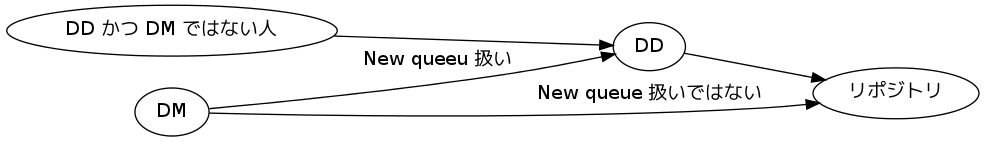
\includegraphics[width=0.8\hsize]{image201108/sponsor0.png}
 \end{center}
\label{fig:sponsor0}\caption{パッケージアップロード}
\end{figure}

\subsection{スポンサーアップロードするときに確認する内容}

パッケージメンテナに「アップロードして!」と言われて、何も考えずに
アップロードしてしまうと変なパッケージがDebianのパッケージ
リポジトリに入ることになり、いろいろ問題が起きてしまいます。
よって、スポンサーはアップロードするパッケージメンテナとパッケージを
確認する必要があります。
スポンサーは確認する前と後にチェックする内容があります。スポンサーによって内容が異なりますが、
ここでは私が行っているチェック内容を紹介します。

\subsubsection{パッケージをチェックする前のチェック}

スポンサーをするパッケージメンテナの方に以下の内容を確認しています。

\begin{itemize}
\item Web of Trust(WOT) に入っているか。

GPGの鍵チェックを行います。WOT に入ってない場合には近くにいるDDにキーサインしてもらうように
依頼しています。

\item DDやDMへの意欲はあるか。

ただパッケージメンテナになるのもいいのですが、私を含めたスポンサーの多くは、
メンテナには最終的に DDになってもらって、Debianの開発に参加して欲しいと思っている
と思います。よって、パッケージメンテナの次のステップについて考えているか、確認しています。
私はDDやDMになりたくないからといって、スポンサーにならないことはないです。

\item Debian 新メンテナーガイド\footnote{\url{http://www.debian.org/doc/manuals/maint-guide/}} を読んだか。
\item DFSG \footnote{\url{http://www.debian.org/social_contract.ja.html}} を読んだか。
\item Debian Policy\footnote{\url{http://www.debian.org/doc/debian-policy/}} を読んだか。
\item Debian Reference \footnote{\url{http://www.debian.org/doc/manuals/developers-reference/}}を読んだか。

これらは読んでおくべきドキュメント類です。読んでないと話
にならないので、まず読んである程度理解してもらうようにしています。

\end{itemize}

これ以外にも、たまに誰もスポンサーする人がいないようなのでスポンサーする場合があります。

\subsubsection{パッケージのチェック}

次に実際のパッケージのチェックを行います。
内容は以下になります。

\begin{itemize}

\item ライセンスの確認

ソフトウェアのライセンスがDFSGに合致するライセンスか、
ライセンスが debian/copuright に書かれているか確認します。
この確認には devscripts パッケージに含まれる licensecheck を使うことが多いです。

また、最近ではdebian/copyright のフォーマットには、
DEP5
\footnote{\url{http://dep.debian.net/deps/dep5/}}
に対応しているか確認しています。
仮に不明な場合には上流開発者に問い合わせるようにメンテナにお願いします。

\item orig.tar.gz の確認

オリジナルのtarボールと一緒か、オリジナルのソースコードに
変な改変をしていないかを確認します。

\item 最新のパッケージングのルールに合っているかの確認。

例えば、使っているプログラミング言語向けのパッケージングサポートツールが新しくなっていたり、
パッケージングポリシーが決まっている場合があります。できるだけ新しいパッケージングのルールに
合わせるようにします。

\item debian/control ファイルの確認

依存関係、パッケージの説明、各セクションの確認を行います。

\item debian/rules の確認

シンプルな構成になっているか、ポリシーに違反していないかの確認。

\item pbuilder を使ったパッケージビルドの確認

最新unstable ディストリビューションでパッケージがビルドできるか確認します。
lintian によるチェックや、ビルドに必要なパッケージが依存関係から漏れていないか
確認することができます。
この時に使うツールは pbuilder\footnote{\url{http://packages.qa.debian.org/p/pbuilder.html}}(cowbuilder\footnote{\url{http://packages.qa.debian.org/c/cowdancer.html}})と、
sbuild\footnote{\url{http://packages.qa.debian.org/s/sbuild.html}} です。
手元でビルドしてアップロードする場合には pbuilder を使っています。
スポンサーをしているパッケージは定期的にビルドの確認を行うようにしており、
これには sbuild を使っています。

\item lintianを使ったポリシーとパッケージングミスの確認

パッケージが Debian ポリシー に準拠しているか簡単に確認するには
lintian\footnote{\url{http://packages.qa.debian.org/l/lintian.html}} を使います。
これはDebian ポリシー の他に Debian パッケージのよくある間違いに関してチェックしてくれます。

\item メンテナスクリプト(preinst、postinst、prerm、postrm、コンフィグ)の確認

これらは動くのか、必要なものなのかをチェックします。

\item オリジナルの tar ボールとの差分の確認

diff.gz の内容を確認します。
作成されたパッチは上流開発者に送ってあるか、パッチはDEP3
\footnote{\url{http://dep.debian.net/deps/dep3/}}
に対応しているか、確認します。

\item パッケージのインストール、アンインストール、動作確認

パッケージはできても、インストールできない場合やアンインストールできない場合があります。
またパッケージが動作しない場合もあります。このような問題
がないか確認するために、
piuparts\footnote{\url{http://packages.qa.debian.org/p/piuparts.html}} を使ってインストール、アンインストールのチェックと、実際にインストールしてみて動作するか確認をします。

\end{itemize}

\subsubsection{その他}
その他、スポンサーによっては以下のような理由でスポンサーしてくれない場合があるようです。
注意しましょう。

\begin{itemize}

\item スポンサーをUploaderに入れることを要求される場合がある。

これは、パッケージメンテナの代わりにパッケージをアップロードする場合に有効です。
先に説明したように、パッケージのメンテナンスの責任はスポンサーにもあるのためです。

\item パッケージング用のツールを要求される場合がある。

例えばスポンサーによっては、パッケージにcdbs を使っている場合、debhelper を使うように言われる場合があるようです。

\item \url{http://mentors.debian.net} を使わない場合はスポンサーをしない。

信頼できる以外にアップロードされたソースパッケージは信頼しないというポリシーのようです。

\item 自分の知らないプログラミング言語で書かれたパッケージはスポンサーをしない。

\end{itemize}

また、\url{http://wiki.debian.org/SponsorChecklist}
に実際にスポンサーしている人の方針が纏められています。

\subsection{アップロード}
アップロードには、dput や dupload パッケージを使います。
実装が異なるだけで、基本的な機能は揃っているのでどちらでも使い方は同じです。

\subsection{まとめ}
以上のようにスポンサーになることはとても大変なので、メンテナの方はさっさとDMかDDがになりましょう。

% 201109 tokyo debian温泉のため無し


%$
\clearpage
% 201111 tokyo OSC Tokyoのため資料無し

% 201111 kansai KOFのため資料無し

% FIXME: quizを追加すること
\dancersection{Debian Trivia Quiz}{上川 純一}

ところで、みなさん Debian 関連の話題においついていますか?Debian関連の話
題はメーリングリストをよんでいると追跡できます。ただよんでいるだけではは
りあいがないので、理解度のテストをします。特に一人だけでは意味がわからな
いところもあるかも知れません。みんなで一緒に読んでみましょう。


\begin{multicols}{2}
 %; whizzy-master ../debianmeetingresume201101.tex
% 以上の設定をしているため、このファイルで M-x whizzytex すると、whizzytexが利用できます。
%
% ちなみに、クイズは別ブランチで作成し、のちにマージします。逆にマージし
% ないようにしましょう。
% (shell-command "git checkout quiz-prepare")

\santaku
{alioth.debian.orgが2台に分かれました。そのサーバ名は?}
{vasks.debian.org と wagner.debian.org}
{volks.debian.org と don.debian.org}
{dennys.debian.org と gusto.debian.org}
{A}
{ほかはファミレスの名前}

\santaku
{現在行われているPerl transition のPerlバージョンは?}
{5.12}
{5.13}
{5.14}
{A}
{5.14はまだexperimentalです。}

\santaku
{プライマリミラーサーバが新しく追加された国は?}
{チュニジア}
{中国}
{マダガスカル}
{B}
{チュニジアとマダカスカルはミラー。プライマリではない。}

\santaku
{mentors.debian.net を構築しているwebアプリケーションが変更されました。何に変わったでしょう?}
{Debmemtors}
{Debcomike}
{Debexpo}
{C}
{Python とTurbogears で
書かれたWebアプリケーション。
パッケージレビューやテストスィートを提供するらしい。}

\santaku
{debian-ports に追加された新しいアーキテクチャは?}
{s390x}
{ppc64}
{blackfin}
{A}
{s390x。aurel32 によって開始。blachfinはまだサポートされていない。}

\santaku
{新しくサポートされた圧縮形式は?}
{rar}
{cab}
{xz}
{C}
{可逆圧縮アルゴリズム LZMA
(Lempel-Ziv-Markov chain-Algorithm)を使った圧縮形式。
GNU zip に比べ、
約40\%圧縮率が向上している。
圧縮には時間がかかるが、伸長には時間がかからない。
}

\santaku
{Samuel Thibault がアナウンスした Debian GNU/Hurd の内容は?}
{Wheezy で Debian GNU/Hurd をリリースします!}
{なんつーか、飽きた。}
{DVDが読めないのでDVDイメージは配布しません。}
{A}
{Whezzy のリリースゴール対象に入れるようです。PorterBox も用意されました。}

\santaku
{Emdebian Grip はなぜ Debianのリポジトリに入れる事が可能なのか?}
{Debianだから。}
{Freeだから。}
{パッケージの互換性があるから。}
{C}
{Emdebian Grip はパッケージからドキュメントファイルなどのa 
組み込みには必要のないファイルを削除したパッケージ
を提供するディストリビューション。}

\santaku
{mentors.debian.net を構築しているwebアプリケーションが変更されました。何に変わったでしょう?}
{Debmemtors}
{Debcomike}
{Debexpo}
{C}
{Python とTurbogears で
書かれたWebアプリケーション。
パッケージレビューやテストスィートを提供するらしい。}

\santaku
{debian-ports に追加された新しいアーキテクチャは?}
{s390x}
{ppc64}
{blackfin}
{A}
{s390x。aurel32 によって開始。blachfinはまだサポートされていない。}

\santaku
{新しくサポートされた圧縮形式は?}
{rar}
{cab}
{xz}
{C}
{可逆圧縮アルゴリズム LZMA
(Lempel-Ziv-Markov chain-Algorithm)を使った圧縮形式。
GNU zip に比べ、
約40\%圧縮率が向上している。
圧縮には時間がかかるが、伸長には時間がかからない。
}

\santaku
{Samuel Thibault がアナウンスした Debian GNU/Hurd の内容は?}
{Wheezy で Debian GNU/Hurd をリリースします!}
{なんつーか、飽きた。}
{DVDが読めないのでDVDイメージは配布しません。}
{A}
{Whezzy のリリースゴール対象に入れるようです。PorterBox も用意されました。}

\santaku
{Emdebian Grip はなぜ Debianのリポジトリに入れる事が可能なのか?}
{Debianだから。}
{Freeだから。}
{パッケージの互換性があるから。}
{C}
{Emdebian Grip はパッケージからドキュメントファイルなどのa 
組み込みには必要のないファイルを削除したパッケージ
を提供するディストリビューション。}

\santaku
{Debian温泉2011の1日目はいつでしょうか?}
{9/17}
{9/18}
{9/19}
{A}
{さっきの話を聞いて(読んで)いればわかって当然ですね}

\santaku
{8月にDebianは誕生日を迎えました。何周年でしたでしょうか?}
{17}
{18}
{19}
{B}
{今年もお祝いしましたよね}

\santaku
{最新のDebian Newsはいつ発行されたでしょうか?}
{9/17}
{9/18}
{9/19}
{C}
{購読していれば知っていて当然ですね}

\santaku
{10/17の''delegation for the DSA team''で代表団に任命されなかったのは誰でしょう?}
{Faidon Liambotis}
{Luca Filipozzi}
{Nobuhiro Iwamatsu}
{C}
{他に任命されたのは、の全部で合計名です。}

\santaku
{Wheezyフリーズの予定はいつでしょう?}
{2012年4月}
{2012年6月}
{2012年8月}
{B}
{あと6ヶ月ですよ!}

\santaku
{1.16.1がリリースされたdpkgに該当するのはどれ?}
{\texttt{dpkg-buildpackage}コマンドでは \texttt{CFLAGS, CXXFLAGS, LDFLAGS, CPPFLAGS, FFLAGS}の\texttt{export}が必須になった}
{\texttt{dpkg-deb}コマンドに\texttt{--verbose}オプションが追加された}
{Multi-Archフィールドがサポートされた}
{B}
{\texttt{dpkg-buildpackage}ではこれらのオプションが不要になりました。Multi-Archは1.16.2からサポートされる予定です。\texttt{dpkg-deb -x/--extract -v/--verbose}で\texttt{dpkg-deb -X/--xextract}と同じ動きをするようになりました。}

\end{multicols}

% 問題と回答が同じみひらきにならないようにする
\clearpage
\dancersection{Debian Trivia Quiz 問題回答}{上川 純一}

 Debian Trivia Quiz の問題回答です。
 あなたは何問わかりましたか?
 \\
 %回答はdebianmeetingresume2010-natsu.jqzというファイルに生成されるので、
 %それを手動でコピペして使う。
 % ここからコピペ
 % FIXME 問題が全部はいったらコピペすること
 %(progn (next-line 1)(insert-file "debianmeetingresume2011-natsu.jqz") )
1. A : ほかはファミレスの名前\\
2. A : 5.14はまだexperimentalです。\\
3. B : チュニジアとマダカスカルはミラー。プライマリではない。\\
4. C : Python とTurbogears で書かれたWebアプリケーション。パッケージレビューやテストスィートを提供するらしい。\\
5. A : s390x。aurel32 によって開始。blachfinはまだサポートされていない。\\
6. C : 可逆圧縮アルゴリズム LZMA (Lempel-Ziv-Markov chain-Algorithm)を使った圧縮形式。GNU zip に比べ、約40\%圧縮率が向上している。圧縮には時間がかかるが、伸長には時間がかからない。\\
7. A : Whezzy のリリースゴール対象に入れるようです。PorterBox も用意されました。\\
8. C : Emdebian Grip はパッケージからドキュメントファイルなどの組み込みには必要のないファイルを削除したパッケージを提供するディストリビューション。\\
9. C : Python とTurbogears で書かれたWebアプリケーション。パッケージレビューやテストスィートを提供するらしい。\\
10. A : s390x。aurel32 によって開始。blachfinはまだサポートされていない。\\
11. C : 可逆圧縮アルゴリズム LZMA (Lempel-Ziv-Markov chain-Algorithm)を使った圧縮形式。GNU zip に比べ、約40\%圧縮率が向上している。圧縮には時間がかかるが、伸長には時間がかからない。\\
12. A : Whezzy のリリースゴール対象に入れるようです。PorterBox も用意されました。\\
13. C : Emdebian Grip はパッケージからドキュメントファイルなどのa 組み込みには必要のないファイルを削除したパッケージを提供するディストリビューション。\\
14. A : さっきの話を聞いて(読んで)いればわかって当然ですね\\
15. B : 今年もお祝いしましたよね\\
16. C : 購読していれば知っていて当然ですね\\
17. C : 他に任命されたのは、Martin Zobel-Helas,Peter Palfrader,Stephen Gran,Tollef Fog Heenの全部で合計6名です。\\
18. B : あと6ヶ月ですよ!\\
19. B : \texttt{dpkg-buildpackage}ではこれらのオプションが不要になりました。Multi-Archは1.16.2からサポートされる予定です。\texttt{dpkg-deb -x/--extract -v/--verbose}で\texttt{dpkg-deb -X/--xextract}と同じ動きをするようになりました。\\

\printindex

% add page to even number
%\newpage
%\thispagestyle{empty}\mbox{}

\newpage
\thispagestyle{empty}\mbox{}
\newpage

\thispagestyle{empty}
{
\large
\begin{itembox}{\bf 『あんどきゅめんてっど でびあん』について}
本書は、東京および関西周辺で毎月行なわれている『東京エリア Debian 勉強会』および
『関西エリア Debian 勉強会』で
使用された資料・小ネタ・必殺技などを一冊にまとめたものです。
収録範囲は2011/06〜2011/11まで
東京エリアは第78回から第81回まで(第82回はOSC 2011 Tokyo/Fallのため収録無し)、関西エリアは第48回から第52回まで(第53回はKOF 2011のため収録無し)。
% FIXME: 回数を修正すること。
内容は無保証、つっこみなどがあれば勉強会にて。
\end{itembox}
}

\vspace*{15cm}
{\color{dancerlightblue}\rule{\hsize}{1mm}}
\vspace{2mm}

\includegraphics[width=2cm]{image200502/openlogo-nd.eps}
\noindent \Large \bf あんどきゅめんてっど でびあん 2011年冬号\\
\noindent \normalfont 2011年12月31日 \hspace{5mm}  初版第1刷発行\\
\noindent \normalfont 東京エリア Debian 勉強会/関西エリア Debian 勉強会 (編集・印刷・発行)\\
{\color{dancerdarkblue}\rule{\hsize}{1mm}}

\end{document}
